\documentclass[a4paper,12pt,3p]{report}

\usepackage{graphicx}
\usepackage[font=normalsize]{caption}
\usepackage{subcaption}
\usepackage{float}
\usepackage{wrapfig}
\usepackage{amssymb}
\usepackage{listings}
\usepackage{amsmath}
\usepackage{amstext}
\usepackage[linesnumbered,ruled]{algorithm2e}
\usepackage{multicol}
\usepackage{multirow}
\usepackage{enumitem}

\usepackage[bookmarks=false]{hyperref}
\hypersetup{colorlinks,
	linkcolor=blue,
	citecolor=blue,
	urlcolor=blue}
\usepackage{titlesec}
\setcounter{secnumdepth}{4}

%\usepackage{csquotes}
%\usepackage[style=verbose-ibid,backend=bibtex]{biblatex}
%\bibliography{reference}

\titleformat{\paragraph}
{\normalfont\normalsize\bfseries}{\theparagraph}{1em}{}
% \titlespacing*{\paragraph}
% {0pt}{3.25ex plus 1ex minus .2ex}{1.5ex plus .2ex}

\titlespacing{\paragraph}{0pt}{\parskip}{-\parskip}
\titlespacing{\section}{0pt}{\parskip}{-\parskip}
\titlespacing{\subsection}{0pt}{\parskip}{-\parskip}
\titlespacing{\subsubsection}{0pt}{\parskip}{-\parskip}

\graphicspath{ {./images/} }
\usepackage[X2,T1]{fontenc}
\usepackage[utf8]{vietnam}
\usepackage{tabu}

\DeclareTextSymbolDefault{\CYREPS}{X2}
\DeclareTextSymbolDefault{\cyreps}{X2}

\DeclareUnicodeCharacter{0190}{\CYREPS}
\DeclareUnicodeCharacter{025B}{\cyreps}
\usepackage[left=2cm,right=2cm,top=2cm,bottom=3cm]{geometry}
\usepackage{indentfirst}
\usepackage{color, colortbl}
\definecolor{Gray}{gray}{0.9}

\usepackage{graphicx}
\usepackage{verbatim}
\usepackage{latexsym}
\usepackage{mathchars}
\usepackage{setspace}
\usepackage{footnote}

\setlength{\parskip}{\medskipamount}  % a little space before a \par
\setlength{\parindent}{0pt}	      % don't indent first lines of paragraphs

%UHEAD.STY  If this is included after \documentstyle{report}, it adds
% an underlined heading style to the LaTeX report style.
% \pagestyle{uheadings} will put underlined headings at the top
% of each page. The right page headings are the Chapter titles and
% the left page titles are supplied by \def\lefthead{text}.

% Ted Shapin, Dec. 17, 1986

\makeatletter
\def\chapapp2{Chapter}

\def\appendix{\par
 \setcounter{chapter}{0}
 \setcounter{section}{0}
 \def\chapapp2{Appendix}
 \def\@chapapp{Appendix}
 \def\thechapter{\Alph{chapter}}}

\def\ps@uheadings{\let\@mkboth\markboth
% modifications
\def\@oddhead{\protect\underline{\protect\makebox[\textwidth][l]
		{\sl\rightmark\hfill\rm\thepage}}}
\def\@oddfoot{}
\def\@evenfoot{}
\def\@evenhead{\protect\underline{\protect\makebox[\textwidth][l]
		{\rm\thepage\hfill\sl\leftmark}}}
% end of modifications
\def\chaptermark##1{\markboth {\ifnum \c@secnumdepth >\m@ne
 \chapapp2\ \thechapter. \ \fi ##1}{}}%
\def\sectionmark##1{\markright {\ifnum \c@secnumdepth >\z@
   \thesection. \ \fi ##1}}}
\makeatother

%%From: marcel@cs.caltech.edu (Marcel van der Goot)
%%Newsgroups: comp.text.tex
%%Subject: illegal modification of boxit.sty
%%Date: 28 Feb 92 01:10:02 GMT
%%Organization: California Institute of Technology (CS dept)
%%Nntp-Posting-Host: andromeda.cs.caltech.edu
%%
%%
%%Quite some time ago I posted a file boxit.sty; maybe it made it
%%to some archives, although I don't recall submitting it. It defines
%%	\begin{boxit}
%%	...
%%	\end{boxit}
%%to draw a box around `...', where the `...' can contain other
%%environments (e.g., a verbatim environment). Unfortunately, it had
%%a problem: it did not work if you used it in paragraph mode, i.e., it
%%only worked if there was an empty line in front of \begin{boxit}.
%%Luckily, that is easily corrected.
%%
%%HOWEVER, apparently someone noticed the problem, tried to correct it,
%%and then distributed this modified version. That would be fine with me,
%%except that:
%%1. There was no note in the file about this modification, it only has my
%%   name in it.
%%2. The modification is wrong: now it only works if there is *no* empty
%%   line in front of \begin{boxit}. In my opinion this bug is worse than
%%   the original one.
%%
%%In particular, the author of this modification tried to force an empty
%%line by inserting a `\\' in the definition of \Beginboxit. If you have
%%a version of boxit.sty with a `\\', please delete it. If you have my
%%old version of boxit.sty, please also delete it. Below is an improved
%%version.
%%
%%Thanks to Joe Armstrong for drawing my attention to the bug and to the
%%illegal version.
%%
%%                                          Marcel van der Goot
%% .---------------------------------------------------------------
%% | Blauw de viooltjes,                    marcel@cs.caltech.edu
%% |    Rood zijn de rozen;
%% | Een rijm kan gezet
%% |    Met plaksel en dozen.
%% |


% boxit.sty
% version: 27 Feb 1992
%
% Defines a boxit environment, which draws lines around its contents.
% Usage:
%   \begin{boxit}
%	... (text you want to be boxed, can contain other environments)
%   \end{boxit}
%
% The width of the box is the width of the contents.
% The boxit* environment behaves the same, except that the box will be
% at least as wide as a normal paragraph.
%
% The reason for writing it this way (rather than with the \boxit#1 macro
% from the TeXbook), is that now you can box verbatim text, as in
%   \begin{boxit}
%   \begin{verbatim}
%   this better come out in boxed verbatim mode ...
%   \end{verbatim}
%   \end{boxit}
%
%						Marcel van der Goot
%						marcel@cs.caltech.edu
%

\def\Beginboxit
   {\par
    \vbox\bgroup
	   \hrule
	   \hbox\bgroup
		  \vrule \kern1.2pt %
		  \vbox\bgroup\kern1.2pt
   }

\def\Endboxit{%
			      \kern1.2pt
		       \egroup
		  \kern1.2pt\vrule
		\egroup
	   \hrule
	 \egroup
   }	

\newenvironment{boxit}{\Beginboxit}{\Endboxit}
\newenvironment{boxit*}{\Beginboxit\hbox to\hsize{}}{\Endboxit}

\pagestyle{empty}

\setlength{\parskip}{2ex plus 0.5ex minus 0.2ex}
\setlength{\parindent}{0pt}

\makeatletter  %to avoid error messages generated by "\@". Makes Latex treat "@" like a letter

\linespread{1.5}
\def\zzfl@error{Float(s) lost}
\def\submitdate#1{\gdef\@submitdate{#1}}
\def\maketitle{
  \begin{titlepage}{
    %\linespread{1.5}
    \Large TRƯỜNG ĐẠI HỌC BÁCH KHOA HÀ NỘI \\
    %\linebreak
    VIỆN CÔNG NGHỆ THÔNG TIN VÀ TRUYỀN THÔNG \\
    %\linebreak
    *****
    \rm
    \vskip 0.5in
    
\includegraphics[width=0.2 \textwidth]{images/hust} 
    \vskip 0.5in
    \Large \bf ĐỒ ÁN TỐT NGHIỆP\par
    \Large \flushleft Đề tài: \par
    \Large \center \bf \@title \par
  }

  \vskip 0.3in
  \par
 % \begin{flushright}
  {\Large Sinh viên thực hiện: \bf \@author} 
  \vskip 0.1in
  \Large Giảng viên hướng dẫn: \bf TS. Phạm Quang Dũng
%	\end{flushright}
  \par
  \vskip 2in
  \par
  
  \@submitdate
  \vfil
  \end{titlepage}
}

\def\titlepage{
  \newpage
  \centering
  \linespread{1}
  \normalsize
  \vbox to \vsize\bgroup\vbox to 9in\bgroup
}
\def\endtitlepage{
  \par
  \kern 0pt
  \egroup
  \vss
  \egroup
  \cleardoublepage
}

\def\abstract{
  \begin{center}{
    \Large\bf Tóm tắt}
  \end{center}
  \small
  %\def\baselinestretch{1.5}
  \linespread{1.5}
  \normalsize
}
\def\endabstract{
  \par
}

\newenvironment{sameauthor}{
	\cleardoublepage
	\begin{center}{
			\large \bf PHỤ LỤC 1: GIẤY XÁC NHẬN ĐỒNG TÁC GIẢ}
	\end{center}
	\small
	\linespread{1.5}
	\normalsize
}{\cleardoublepage}
\def\endsameauthor{
	\par
}


\newenvironment{acknowledgements}{
  \cleardoublepage
  \begin{center}{
    \large \bf Lời cảm ơn}
  \end{center}
  \small
  \linespread{1.5}
  \normalsize
}{\cleardoublepage}
\def\endacknowledgements{
  \par
}

\newenvironment{dedication}{
  \cleardoublepage
  \begin{center}{
    \large \bf Lời cam đoan}
  \end{center}
  \small
  \linespread{1.5}
  \normalsize
}{\cleardoublepage}
\def\enddedication{
  \par
}

\def\preface{

    \pagestyle{plain}
    \doublespacing
}

\def\body{
    \cleardoublepage    
    \pagestyle{uheadings}
    \tableofcontents
    \pagestyle{plain}
    \cleardoublepage
    \pagestyle{uheadings}
    \listoftables
    \pagestyle{plain}
    \cleardoublepage
    \pagestyle{uheadings}
    \listoffigures
    \pagestyle{plain}
    \cleardoublepage
    \pagestyle{uheadings}
    \lstlistoflistings
    \pagestyle{plain}
    \cleardoublepage
    \doublespacing
}

\pagenumbering{arabic}
\makeatother  %to avoid error messages generated by "\@". Makes Latex treat "@" like a letter


\newcommand{\ipc}{{\sf ipc}}

\newcommand{\Prob}{\bbbp}
\newcommand{\Real}{\bbbr}
\newcommand{\real}{\Real}
\newcommand{\Int}{\bbbz}
\newcommand{\Nat}{\bbbn}

\newcommand{\NN}{{\sf I\kern-0.14emN}}   % Natural numbers
\newcommand{\ZZ}{{\sf Z\kern-0.45emZ}}   % Integers
\newcommand{\QQQ}{{\sf C\kern-0.48emQ}}   % Rational numbers
\newcommand{\RR}{{\sf I\kern-0.14emR}}   % Real numbers
\newcommand{\KK}{{\cal K}}
\newcommand{\OO}{{\cal O}}
\newcommand{\AAA}{{\bf A}}
\newcommand{\HH}{{\bf H}}
\newcommand{\II}{{\bf I}}
\newcommand{\LL}{{\bf L}}
\newcommand{\PP}{{\bf P}}
\newcommand{\PPprime}{{\bf P'}}
\newcommand{\QQ}{{\bf Q}}
\newcommand{\UU}{{\bf U}}
\newcommand{\UUprime}{{\bf U'}}
\newcommand{\zzero}{{\bf 0}}
\newcommand{\ppi}{\mbox{\boldmath $\pi$}}
\newcommand{\aalph}{\mbox{\boldmath $\alpha$}}
\newcommand{\bb}{{\bf b}}
\newcommand{\ee}{{\bf e}}
\newcommand{\mmu}{\mbox{\boldmath $\mu$}}
\newcommand{\vv}{{\bf v}}
\newcommand{\xx}{{\bf x}}
\newcommand{\yy}{{\bf y}}
\newcommand{\zz}{{\bf z}}
\newcommand{\oomeg}{\mbox{\boldmath $\omega$}}
\newcommand{\res}{{\bf res}}
\newcommand{\cchi}{{\mbox{\raisebox{.4ex}{$\chi$}}}}
%\newcommand{\cchi}{{\cal X}}
%\newcommand{\cchi}{\mbox{\Large $\chi$}}

% Logical operators and symbols
\newcommand{\imply}{\Rightarrow}
\newcommand{\bimply}{\Leftrightarrow}
\newcommand{\union}{\cup}
\newcommand{\intersect}{\cap}
\newcommand{\boolor}{\vee}
\newcommand{\booland}{\wedge}
\newcommand{\boolimply}{\imply}
\newcommand{\boolbimply}{\bimply}
\newcommand{\boolnot}{\neg}
\newcommand{\boolsat}{\!\models}
\newcommand{\boolnsat}{\!\not\models}


\newcommand{\op}[1]{\mathrm{#1}}
\newcommand{\s}[1]{\ensuremath{\mathcal #1}}

% Properly styled differentiation and integration operators
\newcommand{\diff}[1]{\mathrm{\frac{d}{d\mathit{#1}}}}
\newcommand{\diffII}[1]{\mathrm{\frac{d^2}{d\mathit{#1}^2}}}
\newcommand{\intg}[4]{\int_{#3}^{#4} #1 \, \mathrm{d}#2}
\newcommand{\intgd}[4]{\int\!\!\!\!\int_{#4} #1 \, \mathrm{d}#2 \, \mathrm{d}#3}

% Large () brackets on different lines of an eqnarray environment
\newcommand{\Leftbrace}[1]{\left(\raisebox{0mm}[#1][#1]{}\right.}
\newcommand{\Rightbrace}[1]{\left.\raisebox{0mm}[#1][#1]{}\right)}

% Funky symobols for footnotes
\newcommand{\symbolfootnote}{\renewcommand{\thefootnote}{\fnsymbol{footnote}}}
% now add \symbolfootnote to the beginning of the document...

\newcommand{\normallinespacing}{\renewcommand{\baselinestretch}{1.5} \normalsize}
\newcommand{\mediumlinespacing}{\renewcommand{\baselinestretch}{1.2} \normalsize}
\newcommand{\narrowlinespacing}{\renewcommand{\baselinestretch}{1.0} \normalsize}
\newcommand{\bump}{\noalign{\vspace*{\doublerulesep}}}
\newcommand{\cell}{\multicolumn{1}{}{}}
\newcommand{\spann}{\mbox{span}}
\newcommand{\diagg}{\mbox{diag}}
\newcommand{\modd}{\mbox{mod}}
\newcommand{\minn}{\mbox{min}}
\newcommand{\andd}{\mbox{and}}
\newcommand{\forr}{\mbox{for}}
\newcommand{\EE}{\mbox{E}}

\newcommand{\deff}{\stackrel{\mathrm{def}}{=}}
\newcommand{\syncc}{~\stackrel{\textstyle \rhd\kern-0.57em\lhd}{\scriptstyle L}~}

\def\coop{\mbox{\large $\rhd\!\!\!\lhd$}}
\newcommand{\sync}[1]{\raisebox{-1.0ex}{$\;\stackrel{\coop}{\scriptscriptstyle
#1}\,$}}

\newtheorem{definition}{Definition}[chapter]
\newtheorem{theorem}{Theorem}[chapter]

\newcommand{\Figref}[1]{Figure~\ref{#1}}
\newcommand{\fig}[3]{
 \begin{figure}[!ht]
 \begin{center}
 \scalebox{#3}{\includegraphics{figs/#1.ps}}
 \vspace{-0.1in}
 \caption[ ]{\label{#1} #2}
 \end{center}
 \end{figure}
}

\newcommand{\figtwo}[8]{
 \begin{figure}
 \parbox[b]{#4 \textwidth}{
 \begin{center}
 \scalebox{#3}{\includegraphics{figs/#1.ps}}
 \vspace{-0.1in}
 \caption{\label{#1}#2}
 \end{center}
 }
 \hfill
 \parbox[b]{#8 \textwidth}{
 \begin{center}
 \scalebox{#7}{\includegraphics{figs/#5.ps}}
 \vspace{-0.1in}
 \caption{\label{#5}#6}
 \end{center}
 }
 \end{figure}
}


\setlength{\parindent}{30pt}

\definecolor{mygreen}{rgb}{0,0.6,0}
\definecolor{mygray}{rgb}{0.5,0.5,0.5}
\definecolor{mymauve}{rgb}{0.58,0,0.82}
 
%Customize a bit the look
\lstset{ %
backgroundcolor=\color{white}, % choose the background color; you must add \usepackage{color} or \usepackage{xcolor}
basicstyle=\footnotesize, % the size of the fonts that are used for the code
breakatwhitespace=false, % sets if automatic breaks should only happen at whitespace
breaklines=true, % sets automatic line breaking
captionpos=b, % sets the caption-position to bottom
commentstyle=\color{mygreen}, % comment style
deletekeywords={...}, % if you want to delete keywords from the given language
escapeinside={\%*}{*)}, % if you want to add LaTeX within your code
extendedchars=true, % lets you use non-ASCII characters; for 8-bits encodings only, does not work with UTF-8
frame=single, % adds a frame around the code
keepspaces=true, % keeps spaces in text, useful for keeping indentation of code (possibly needs columns=flexible)
keywordstyle=\color{blue}, % keyword style
% language=Octave, % the language of the code
morekeywords={*,...}, % if you want to add more keywords to the set
numbers=left, % where to put the line-numbers; possible values are (none, left, right)
numbersep=5pt, % how far the line-numbers are from the code
numberstyle=\tiny\color{mygray}, % the style that is used for the line-numbers
rulecolor=\color{black}, % if not set, the frame-color may be changed on line-breaks within not-black text (e.g. comments (green here))
showspaces=false, % show spaces everywhere adding particular underscores; it overrides 'showstringspaces'
showstringspaces=false, % underline spaces within strings only
showtabs=false, % show tabs within strings adding particular underscores
stepnumber=1, % the step between two line-numbers. If it's 1, each line will be numbered
stringstyle=\color{mymauve}, % string literal style
tabsize=2, % sets default tabsize to 2 spaces
title=\lstname % show the filename of files included with \lstinputlisting; also try caption instead of title
}
%END of listing package%
 
\definecolor{darkgray}{rgb}{.4,.4,.4}
\definecolor{purple}{rgb}{0.65, 0.12, 0.82}
 
%define Javascript language
\lstdefinelanguage{JavaScript}{
keywords={typeof, new, true, false, catch, function, return, null, catch, switch, var, if, in, while, do, else, case, break},
keywordstyle=\color{blue}\bfseries,
ndkeywords={class, export, boolean, throw, implements, import, this},
ndkeywordstyle=\color{darkgray}\bfseries,
identifierstyle=\color{black},
sensitive=false,
comment=[l]{//},
morecomment=[s]{/*}{*/},
commentstyle=\color{purple}\ttfamily,
stringstyle=\color{red}\ttfamily,
morestring=[b]',
morestring=[b]"
}
 
\lstset{
language=JavaScript,
extendedchars=true,
basicstyle=\footnotesize\ttfamily,
showstringspaces=false,
showspaces=false,
numbers=left,
numberstyle=\footnotesize,
numbersep=9pt,
tabsize=2,
breaklines=true,
showtabs=false,
captionpos=b
}


\renewcommand{\baselinestretch}{2.0}
\begin{document}

\title{\LARGE {\bf Thiết kế hệ thống quản lý phân phối \\ trong chuỗi cung ứng}\\
 \vspace*{7mm}
}

\author{Tạ Quang Tùng}
\submitdate{Hà Nội, 6/2020}

\normallinespacing
\maketitle

\preface
\addcontentsline{toc}{chapter}{Abstract}

\begin{abstract}

Trong ngày nay, việc xây dựng, phát triển các ứng dụng áp dụng công nghệ blockchain đều cần thực hiện hai tương tác với nó chính là ghi dữ liệu lên các mạng và đọc dữ liệu từ chúng. Hai công việc này đòi hỏi các nhà phát triển phải có một hiểu biết sâu rộng về công nghệ blockchain, và sẽ là một thách thức lớn hơn khi các nhà lập trình muốn sử dụng nhiều nền tảng blockchain khác nhau cho ứng dụng của mình. Cho đến nay vẫn chưa có bất kỳ một cơ chế nhất quán nào thực hiện đọc và ghi dữ liệu lên những nền tảng blockchain hiện có. Để giải quyết vấn đề này, tôi đề xuất trong đồ án một ngôn ngữ ánh xạ dữ liệu được đặt tên BML. BML cho phép nhà phát triển định nghĩa một cách nhất quán ánh xạ cho việc chuyển đổi dữ liệu từ các dạng lưu trữ dữ liệu truyền thống lên trên mạng blockchain. Hơn thế nữa, BML cũng hỗ trợ người dùng đọc những dữ liệu đã được lưu trữ trên mạng. Hiện tại, BML hỗ trợ chuyển đổi dữ liệu với năm loại dữ liệu đầu vào phổ biến, bao gồm XML, JSON, XLSX, SQL (cơ sở dữ liệu quan hệ), NoSQL (cơ sở dữ liệu phi quan hệ) đến hai nền tảng blockchain khác nhau, bao gồm Ethereum và Hyperledger Sawtooth. Trong đồ án  này, tôi giới thiệu thiết kế và triển khai của BML, sau đó thực hiện các đánh giá hiệu quả của ngôn ngữ trên các khía cạnh về hiệu năng, tính mở rộng, độ bảo mật và phi tập trung.

\end{abstract}

\cleardoublepage

\addcontentsline{toc}{chapter}{Lời cảm ơn}

\begin{acknowledgements}

Đầu tiên, em xin được gửi lời cảm ơn chân thành đến các thầy giáo,
cô giáo thuộc trường đại học Bách Khoa Hà Nội, đặc biệt là các thầy
giáo, cô giáo thuộc Viện Công nghệ Thông tin và Truyền Thông đã tận
tình dạy dỗ và trang bị cho em những kiến thức bổ ích trong năm năm vừa qua.

Đồng thời em cũng xin được gửi lời cảm ơn đặc biệt đến TS Nguyễn Bình Minh.
Thầy là người đã chỉ dẫn tận tình, cho em những kinh nghiệm quý báu
để có thể hoàn thành đồ án này.

Em xin gửi lời cảm ơn tới gia đình và bạn bè đã sát cánh,
động viên và hỗ trợ em trong suốt những năm qua. 

AFBDF

\end{acknowledgements}


\body
% body of thesis comes here

\chapter{GIỚI THIỆU ĐỀ TÀI}

\section{Đặt vấn đề}
Hiện nay, với sự phát triển kinh tế và sự phát triển của thương mại
điện tử, lượng hàng hóa cung và cầu càng ngày càng lớn. Kéo theo lượng
hàng hóa lớn đó là vấn đề phân phối và quản lý sao cho hiệu quả. Khi hàng
hóa nhiều lên, các phương pháp quản lý kho cũ không còn đáp ứng được
thì mỗi công ty hay tập đoàn phân phối bán lẻ đều cần phải đưa ra giải pháp
mới để quản lý hàng hóa.

Hệ thống quản lý phân phối (Distribution Management System) là một ứng dụng
cung cấp giải pháp cho vấn đề này. Với hệ thống quản lý phân phối,
các công ty hay tập đoàn bán lẻ có thể nắm
được chính xác biến động thị trường,
hàng hóa đang ở vị trí nào trong chuỗi cung ứng, hàng tồn kho còn bao
nhiêu hay hiệu suất làm việc của các nhân viên bán hàng, …

Cùng với vấn đề quản lý một lượng ngày càng lớn các hàng hóa là sự phức
tạp của các hệ thống quản lý phân phối (DMS) ngày càng cao. Nhờ sự
phát triển của công nghệ trong thời gian hiện nay, đặc biệt là công nghệ
Web đã tạo ra nhiều hướng đi, giải pháp mới trong xây dựng các hệ thống
thông tin nói chung và DMS nói riêng. Tuy nhiên, với những doanh nghiệp
đã và đang sử dụng những công nghệ không còn phổ biến, việc thay đổi
công nghệ luôn là một điều khó khăn.

\section{Mục tiêu và phạm vi đề tài}
Từ sự cần thiết phải chuyển đổi phương pháp quản lý phân phối, nhiều phần
mềm nghiệp vụ đã được triển khai. Ở Việt Nam hiện nay, các ứng dụng
quản lý bán lẻ trực tuyến phổ biến có thể kể đến như KiotViet, Sapo, Suno,
... Các ứng dụng quản lý không cần trực tuyến như Adaline, BS Silver,
Perfect Warehouse, ... Các ứng dụng quản lý bản lẻ này tuy cũng có
những tính năng như quản lý sản phẩm, đơn hàng, ... tuy nhiên lại đơn giản
so với một hệ thống quản lý phân phối đầy đủ của một doanh nghiệp lớn về
phân phối hàng hóa.

Do sự phức tạp ngày càng cao của các hệ thống quản lý phân phối, tốc độ
triển khai phát triển hệ thống cũng như hiệu năng của hệ thống ngày cảm
suy giảm. Các công nghệ mới đang dần trở thành xu hướng hiện nay có tiềm
năng để giải quyết những vấn đề trên. Tuy nhiên, các doanh nghiệp đôi
khi cũng không sẵn sàng cho việc thay đổi đó.

Vì vậy, chúng tôi muốn xây dựng một ứng dụng quản lý phân phối riêng biệt,
áp dụng công nghệ phát triển và triển khai mới nhất, có đánh giá định tính
nhằm xác định và cải thiện hiệu năng hệ thống, có phương pháp xây dựng
nhằm khai thác được lợi thế của các dịch vụ Cloud. Ứng dụng quản lý
phân phối của chúng tôi sẽ tập trung vào 8 tính năng chính,
đó là phân quyền động, quản lý tài khoản, quản lý sản phẩm, quản lý kho,
quản lý xuất nhập, quản lý đơn hàng, quản lý tuyến bán
hàng và quản lý nhân viên bán hàng.

\section{Định hướng giải pháp}
Go là một ngôn ngữ lập trình mới do Google phát triển,
được sinh ra để giúp ngành công nghiệp phần mềm khai thác nền
tảng đa lõi của bộ vi xử lý và hoạt động đa nhiệm tốt hơn.
Vì vậy chúng tôi sử dụng Go để viết back-end server nhằm tăng hiệu
năng xử lý yêu cầu trên một thời điểm.

Còn về phần giao diện, giao tiếp với người dùng (front-end) thì hiện
nay các Framework Javascript như ReactJS, Angular hay VueJS đang
là xu thế bởi khả năng xây dựng giao diện nhanh, bảo trì và
mở rộng code dễ dàng. Ứng dụng của chúng tôi sử dụng ReactJS, kết hợp Redux và
Material-UI để xây dựng giao diện đảm bảo thiết kế
chuẩn Material Design của Google. 

Về cơ sở dữ liệu, chúng tôi sử dụng PostgreSQL vì đó là phần mềm mã nguồn
mở có hiệu năng và tính mở rộng cao. Đồng thời sử dụng Redis làm nơi lưu
trữ thông tin phiên làm việc (session) và dữ liệu cache.
Chúng tôi sử dụng một công nghệ container đang được
ưa chuộng là Docker và công nghệ điều phối là Kubernetes để xây dựng
và triển khai ứng dụng. Còn về dịch vụ cloud, chúng tôi sử dụng Microsoft
Azure làm nhà cung cấp dịch vụ cloud chính để ứng dụng chạy trên.

Để có thể đánh giá hiệu năng hệ thống, chúng tôi kết hợp đánh giá hiệu năng
dựa vào công cụ có trên PostgreSQL và dựa vào chương trình dòng lệnh viết
bằng Go để giả lập các truy cập từ người dùng.

\section{Bố cục đồ án}
Phần còn lại của báo cáo đồ án tốt nghiệp được tổ
chức thành các chương như sau.

Chương 2 trình bày về cơ sở lý thuyết của đồ án. Trong đó bao gồm
các công nghệ cốt lõi đã tìm hiểu để xây dựng ứng dụng, so sánh
giữa các công nghệ được sử dụng với các công nghệ khác hiện nay.
Bên cạnh đó là các thuật toán cơ sở được sử dụng trong xử lý logic
cho cả phần front-end, back-end và cơ sở dữ liệu như Index,
Role-Based Access Control, thuật toán phân cụm. 

Chương 3 trình bày chi tiết về thiết kế hệ thống. Từ sự cần thiết
của giải pháp đã nêu ở trên, chúng tôi xác định ra những tính năng cần thiết
nhất và xây dựng các ca sử dụng xung quanh những tính năng này.
Phần này sẽ trình bày các biểu đồ ca sử dụng cho các chức năng,
biểu đồ hoạt động thể hiện cách thức tương tác với hệ thống của
người dùng. Cùng với đó là thiết kế cơ sở dữ liệu, xây dựng dữ liệu mẫu.

Chương 4 đưa ra đóng góp chính của chúng tôi trong đồ án tốt nghiệp này,
so sánh chúng với những giải pháp hiện tại, cơ hội áp dụng trong
tương lai và khả năng mở rộng của đóng góp này. Chương này cũng
đưa ra những vấn đề và hướng giải quyết của những vấn đề này
trong quá trình thực hiện đồ án đồng thời 
minh họa các chức năng của hệ thống.

Chương 5 mô tả quy trình triển khai ứng dụng lên cloud.
Đánh giá hiệu năng hệ thống bằng stress test và performance test
thông qua cơ sử dữ liệu và REST API. 

Chương 6 là chương cuối cùng đưa ra kết luận, những vấn đề còn
chưa giải quyết được và hướng phát triển của ứng dụng trong tương lai.

\chapter{CƠ SỞ LÝ THUYẾT VÀ CÔNG NGHỆ SỬ DỤNG}

\section{Giải pháp quản lý phân phối}
\subsection{Các khái niệm trong quản lý phân phối}
Trước tiên, ta cần tìm biết về một từ khóa đã trở nên rất
phổ biến trong thời gian gần đây,
đó là Logistics~\cite{logistics:online}. Hiểu một cách đơn
giản thì Logistics là quá trình lên kế hoạch, áp dụng và kiểm soát
các luồng dịch chuyển của hàng hóa hay thông tin liên quan tới nguyên
nhiên liệu vật tư (đầu vào) và sản phẩm cuối cùng (đầu ra) từ thời
điểm xuất phát tới điểm tiêu thụ. Đi kèm với Logistics là khái niệm
về Quản trị chuỗi cung ứng (Supply Chain Management), Quản trị chuỗi
cung ứng bao gồm tất cả những hoạt động quản trị logistics cũng như
những hoạt động sản xuất và thúc đẩy sự phối hợp về quy trình và
hoạt động của các bộ phận marketing, kinh doanh, thiết kế sản phẩm,
tài chính, công nghệ thông tin. Khái niệm chuỗi cung ứng rộng hơn,
bao gồm cả logistics và quá trình sản xuất. Ngoài ra chuỗi cung ứng
chú trọng hơn đến hoạt động mua hàng (procedurement) trong khi
logistics giải quyết các vấn đề chiến lược, phối hợp giữa marketing và
sản xuất.

Khi đã có một hình dung cơ bản về chuỗi cung ứng, ta đến với
phần chính là \textbf{hệ thống quản lý phân phối}
(Distribution Management System). Hệ thống quản lý phân phối
(Distribution Management System) là phần mềm quản lý chuỗi
cung ứng hàng hóa của doanh nghiệp, giúp họ quản lý các hoạt
động phân phối hàng hóa ra thị trường, kiểm soát các kênh phân
phối, quản lý nhân viên, người bán hàng, kiểm soát hàng hóa
trong kho, hàng tồn kho, kế hoạch vận chuyển
hàng hóa đến địa chỉ mua hàng,…

Ví dụ, Masan Group là một công ty lớn trong lĩnh vực kinh tế
tư nhân Việt Nam, tập trung hoạt động trong ngành hàng tiêu dùng và
tài nguyên của Việt Nam. Masan quản lý các nền tảng kinh doanh có
quy mô lớn nhằm phát triển và khai thác các tiềm năng trong lĩnh vực
tiêu dùng và tài nguyên. Còn rất nhiều những tập đoàn bán lẻ khác
có cùng cơ chế quản lý kinh doanh như Masan, mỗi tập đoàn như vậy đều
cần có một hệ thống riêng để quản lý chuỗi cung ứng của mình.

Vì vậy Distribution Management System là một trong số những
phần mềm quản lý doanh nghiệp có tính ứng dụng cao, phù hợp với mọi
doanh nghiệp sản xuất và phân phối. Đối với các doanh nghiệp lớn
(ví dụ Masan, VinGroup) có đội ngũ nhân viên bán hàng đông đảo và các
kênh phân phối phức tạp, phần mềm DMS càng quan trọng và là công cụ không
thể thiếu. Các nhà quản lý của các tập đoàn lớn này luôn đau đầu vì
những câu hỏi như “Làm thế nào để nắm được nhanh nhất xu thế, biến động
của thị trường?”, “Làm thế nào để kiểm soát phân phối tốt, duy
trì tồn kho ở mức tối ưu, tiết kiệm thời gian?”, “Tự động hóa bán
hàng, tăng hiệu quả bán hàng cho đội ngũ nhân viên bán hàng như
thế nào?”. Với hệ thống quản lý kênh phân phối (DMS), các doanh nghiệp
lớn với vài trăm, hoặc vài nghìn nhân viên bán hàng, hàng chục
nghìn điểm bán sẽ dễ dàng làm được việc này.

\subsection{Lợi ích của hệ thống quản lý phân phối}
Phần trên đã trình bày về lý do tại sao các doanh nghiệp và tập
đoàn bán lẻ phải sử dụng giải pháp quản lý phân phối và sau đây
là những lợi ích chính, thấy rõ nhất theo như tìm hiểu của chúng tôi.

Thứ nhất Distribution Management System~\cite{dms:online}
là công cụ tự động hóa
bán hàng, giúp nhân viên bán hàng (salesman) tiết kiệm thời gian,
tăng chất lượng chăm sóc khách hàng, tối ưu doanh thu. Mọi thông
tin nhân viên bán hàng cần khi ghé thăm một điểm bán lẻ (rental outlet) 
bao gồm thông tin về khách hàng (customer), lịch sử mua hàng, 
các báo cáo bán hàng, thông tin sản phẩm, chương trình khuyến mãi,… 
có sẵn trong ứng dụng di động DMS để nhân viên có thể dễ dàng theo
dõi tại điểm bán.

Thứ hai Distribution Management System có thể quản lý hiệu quả
làm việc của nhân viên bán hàng, nhà quản lý có thể nắm được lộ
trình ghé thăm khách hàng của nhân viên trên bản đồ lịch sử checkin.
Thông qua đó đánh giá được nhân viên bán hàng có đang tích cực
ngoài thị trường hay không, khách hàng có được chăm sóc tốt hay không.

Thứ ba, đặc biệt hơn là qua hệ thống nhà quản trị sẽ biết
được những cửa hàng nào đang liên tục phát sinh doanh số, những cửa hàng
nào lâu rồi chưa phát sinh đơn hàng mới. Từ đó có thể sắp xếp,
phân chia hợp lý các nhân viên bán hàng vào các tuyến bán
hàng, thay đổi tần suất viếng thăm khách hàng cho phù hợp với
thực tế, tránh lãng phí nguồn lực đồng thời có thể chăm sóc được kỹ
hơn các cửa hàng trọng tâm.

Thứ tư, cập nhật thị trường là điểm nổi bật của phần mềm 
Distribution Management System. Giúp các doanh nghiệp phân phối có thể
kiểm soát được hàng tồn tại từng điểm bán lẻ, đại lý nhằm
đưa ra kế hoạch sản xuất, điều phối hàng hóa phù hợp.

\section{Lý thuyết và công nghệ}
\subsection{Role-Based Access Control}
Trong an toàn thông tin, role-based access control (RBAC) là
một cách tiệp cận cho vấn đề hạn chế quyền truy cập của
người dùng. RBAC được sử dụng phổ biến tại các tổ chức
lớn với nhiều hơn 500 nhân viên. 

RBAC có nhiều mô hình khác nhau. Mô hình cơ bản là
$\text{RBAC}_0$, mô hình có chứa quan hệ phân cấp là
$\text{RBAC}_1$, có chứa ràng buộc $\text{RBAC}_2$ và mô hình tăng
cường (consolidated) $\text{RBAC}_3$~\cite{rbac}.

Các thành phần chính của RBAC bao gồm user (người dùng),
role (vai trò), permission (quyền) và session (phiên truy cập)
cùng với quan hệ giữa chúng nhằm đơn giản hóa quá trình
gán quyền cho người dùng. 

User hay người dùng trong mô hình RBAC là con người, tuy nhiên
khái niệp này có thể được tổng quát hóa bằng việc bao gồm cả những
tác nhân tự động như robot hay phần mềm khác. Một role là một
chức năng công việc hay chức vụ trong tổ chức đi kèm với các
thẩm quyển mà nhân viên trong chức vụ đó nắm giữ. Còn một
permission là sự một chấp nhận cho một phương thức truy cập
vào một hay nhiều các đối tượng trong hệ thống. Việc một
permission tương ứng với gì thì tùy thuộc vào hệ thống
implement ra sao mô hình RBAC.

Mỗi một session là một ánh xạ từ mỗi phần tử của tập user
sang tập con của tập các role. Session thiết lập một phiên
truy cập với tập các role được kích hoạt (là một tập con
của tập các role mà người dùng đó được gán). Mỗi một phiên truy
cập tương ứng cho một user, trong $\text{RBAC}_0$ sự tương ứng này
là không thay đổi theo thời gian.

Trong RBAC, permission được gán với một hoặc nhiều role,
người dùng hay nhân viên được gán với một hay nhiều role.
Người dùng trong RBAC không được gán trực tiếp các permission mà
phải thông qua role, từ đó đơn giản hóa quá trình gán
permission hay việc chuyển phòng ban công tác của nhân viên. 

Trong đồ án này chỉ sử dụng mô hình điều khiển truy cập
dựa trên $\text{RBAC}_0$, biểu diễn toán học của $\text{RBAC}_0$ như sau:
\begin{itemize}[topsep=0ex]
\item Tập $U$, $R$, $P$ và $S$ tương ứng với tập hợp của các
    user, role, permission và session.
\item Tập $PA \subseteq P \times R$ biểu diễn quan hệ nhiều nhiều
    giữa permission và role.
\item Tập $UA \subseteq U \times R$ biểu diễn quan hệ nhiều nhiều giữa user và role.
\item Ánh xạ $user: S \rightarrow U$ gán mỗi một
    session $s$ cho một user $user(s)$.
\item Ánh xạ $roles: S \rightarrow \mathcal{P}(R)$ gán mỗi một
    session $s$ cho tập con của các role: 
    $roles(s) \subseteq \{ r | \left( user(s), r \right) \in UA \}$
    (có thể thay đổi theo thời gian) và session sẽ có các permission
    là $\bigcup_{r \in roles(s)}  \{ p | (p, r) \in PA \}$
\end{itemize}

\begin{figure}[H]
\centering
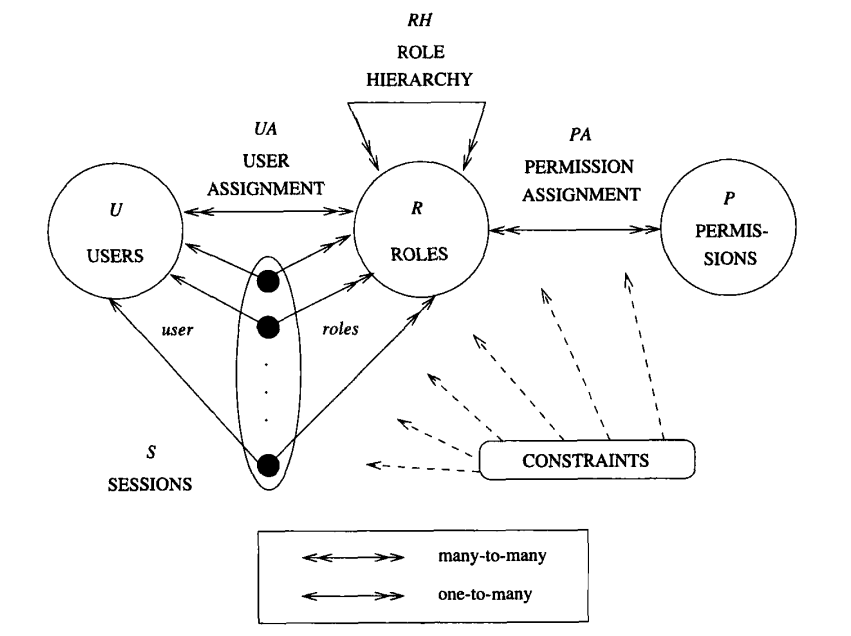
\includegraphics[width=12cm]{images/RBAC.png}
\caption{Các mô hình RBAC}
\end{figure}

\subsection{Công nghệ front-end}
\subsubsection{ReactJS}
\paragraph{Khái quát về ReactJS}
Ngày nay ReactJS~\cite{reactjs:online} đã trở nên rất phổ biến bởi những tính năng
linh hoạt và đơn giản với hơn 1.300.000 developer và hơn 94.000
trang web đang sử dụng ReactJS
(theo số liệu thống kê trên blog topdev.vn). 
ReactJS là một thư viện JavaScript mã nguồn mở được thiết kế
bởi Facebook để tạo ra những ứng dụng web hấp dẫn, nhanh và
hiệu quả với source code tối thiểu. Mục đích cốt lõi của
ReactJS không chỉ khiến cho trang web phải thật mượt mà còn
phải nhanh, khả năng mở rộng cao và đơn giản. Trên website chính
thức của React tổng quan rằng: ReactJS –
“A JavaScript for library for building user interface”,
tức là React sinh ra để phục vụ tầng View,
tập trung vào xây dựng giao diện. 

Tư tưởng của ReactJS là xây dựng lên các component có
tính tái sử dụng, dễ dàng cho việc chia nhỏ vấn đề, kiểm thử,
giúp chúng ta dễ dàng quản lý, mở rộng hệ thống. Đặc tính của
ReactJS là luôn giữ các component ở trạng thái stateless nhiều
nhất có thể, khiến ta dễ dàng quản lý nó. Bản thân các component
này không có trạng thái, nó nhận đầu vào từ bên ngoài và
chỉ hiển thị ra dựa vào các đầu vào đó, điều này
cũng lý giải tính tái sử dụng (reuse) và tiện lợi
trong kiểm thử (testing) của ReactJS.

\paragraph{Virtual DOM}
Sử dụng ReactJS, ta thường hay nghe tới Virtual DOM~\cite{virtualdom:online},
DOM thì rất quen thuộc với những lập trình viên front-end,
còn Virtual DOM là gì? Có khác gì với DOM không? 

Trước tiên, DOM là viết tắt của Document Object Model là
một chuẩn được định nghĩa bởi W3C dùng để truy xuất và thao
tác trên code HTML bằng các ngôn ngữ lập trình thông dịch
(scripting language) như JavaScript.

Khi DOM thay đổi, trình duyệt phải tính toán lại CSS và dựng lại
trang web, điều này sẽ tốn thời gian, nhất là với những ứng dụng
Single Page Application, việc sửa đổi DOM là liên tục không ngừng
nghỉ. Hay khi xử lý các sự kiện (event) như click, submit, …
DOM sẽ tìm tất cả các node liên quan đến sự kiện và cập nhật nếu
thấy nó cần thiết. Vậy thì có cần thiết khi phải tìm tất
cả các node liên quan không? Hay sẽ hiệu quả hơn khi chỉ tìm
node nào cần cập nhật.

\begin{figure}[H]
\centering
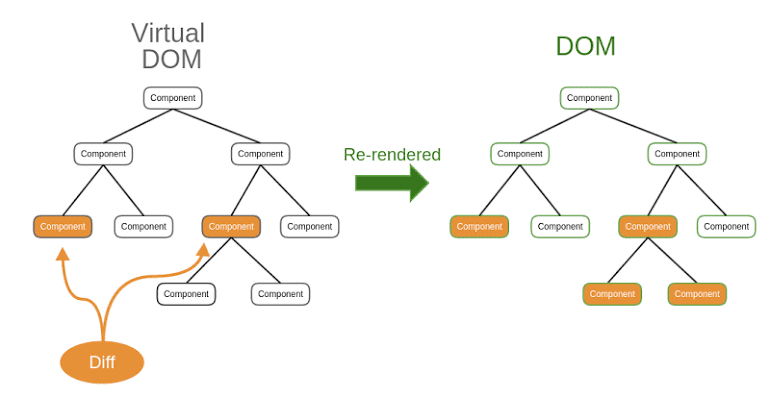
\includegraphics[width=\textwidth]{images/DOM.png}
\caption{Virtual DOM Snapshots \& Diffing}
\label{fig:virtualdom}
\end{figure}

Virtual DOM xuất hiện để giải quyết những vấn đề này.
Virtual DOM gắn với ReactJS, thay vì xử lý DOM Tree thủ công,
chúng định nghĩa các component trông giống DOM
(vì vậy mà cú pháp JSX nhìn rất giống HTML), còn ReactJS sẽ thực
hiện công việc ở tầng thấp hơn. Tổng quát thì Virtual DOM là
một định dạng dữ liệu JavaScript nhẹ dùng để thể hiện nội dung
của DOM tại một thời điểm nhất định nào đó. Nó có tất cả các thuộc
tính giống như DOM nhưng không có khả năng tương tác lên màn hình như
DOM. Sự đặc biệt của Virtual DOM nằm ở cơ chế Snapshots và Diffing.
Khi cần cập nhật phần tử giao diện, React sẽ lấy một snapshot của Virtual
DOM (có thể hiểu là bản ghi trạng thái ngay lúc đó),
sử dụng snapshot này để so sánh với một Virtual DOM trước
khi thực hiện thay đổi.
\paragraph{Single Page Application (SPA)}
Với ReactJS, ta dễ dàng tạo ra một Single Page Application (SPA).
Khác với những ứng dụng web truyền thống, Single Page Application
có một trang gốc và trong trang gốc đó, chúng ta có thể tải
nhiều trang con (tương ứng với các thành phần của trang gốc) mà
không gây bất kì ảnh hưởng gì đến trang gốc. Trong khi các
ứng dụng web truyền thống phải tải lại toàn bộ trang khi
chúng ta tương tác với trang web thì Single Page Application chỉ load
phần trang cần thiết. Các thành phần chung như header, footer, menu,
side bar,… thường xuất hiện ở nhiều trang của ứng dụng sẽ được
Single Page Application load một lần duy nhất ở trang gốc.

\begin{figure}[H]
\centering
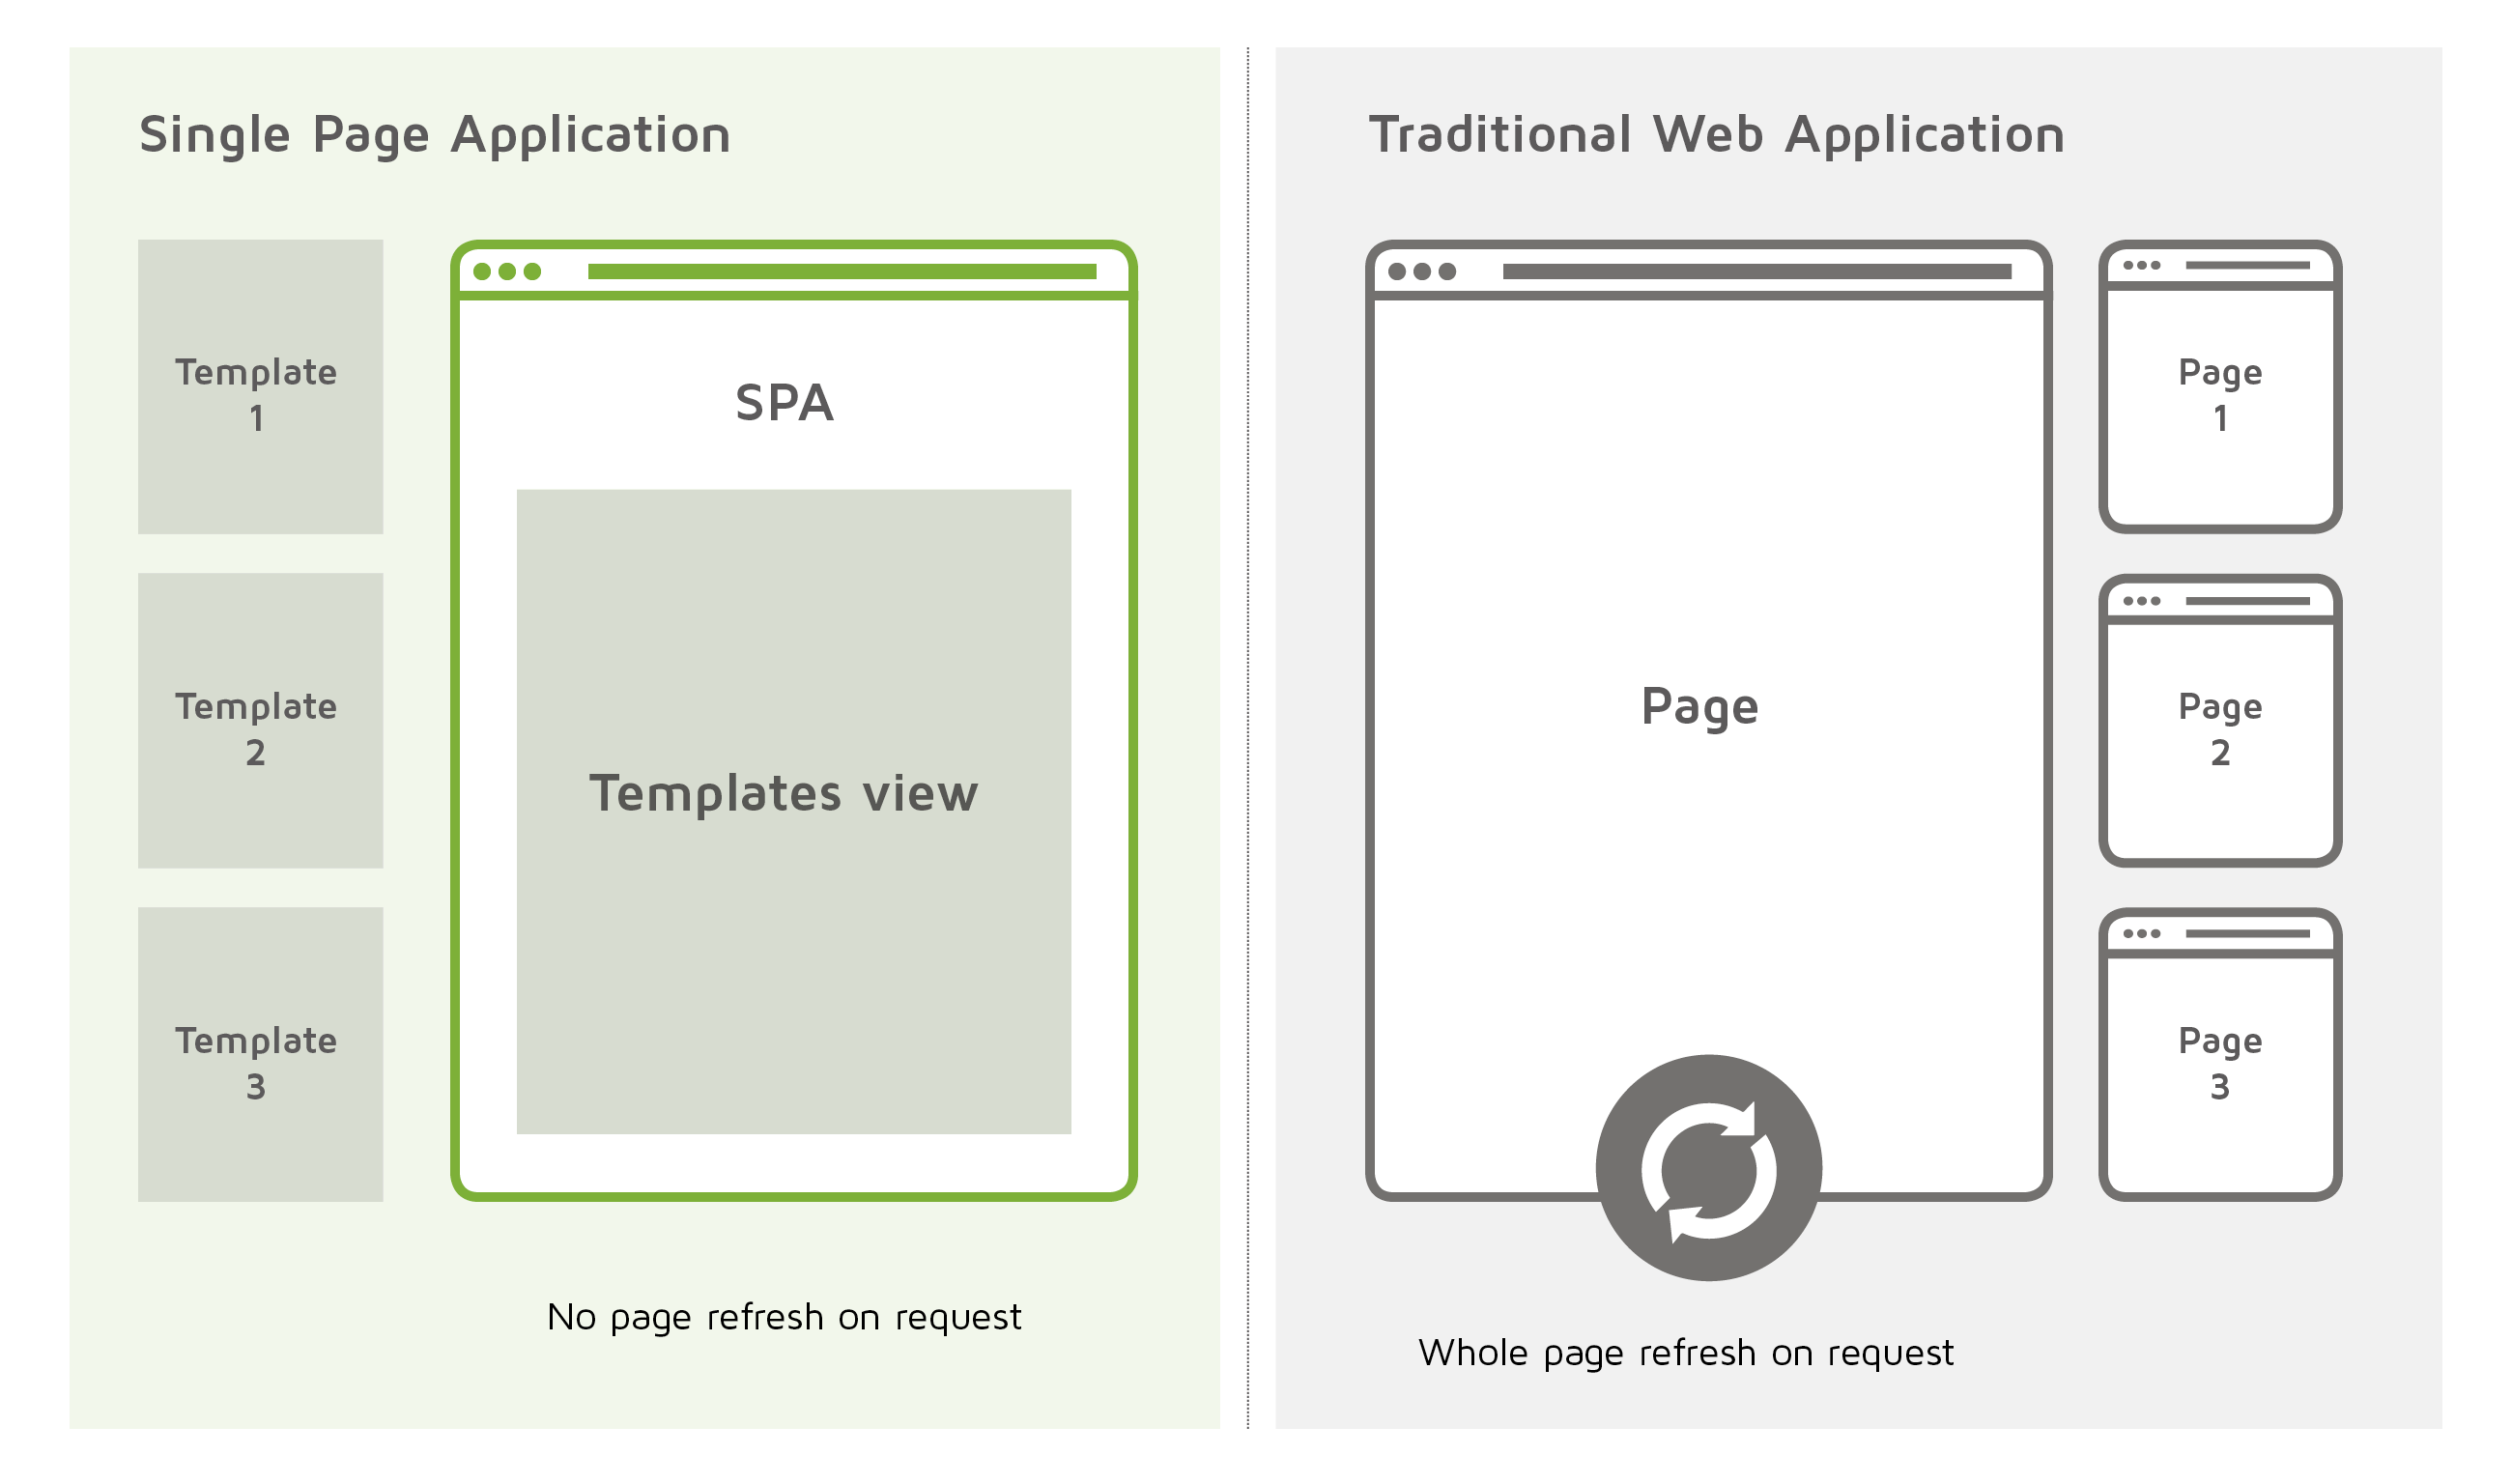
\includegraphics[width=\textwidth]{images/single-page-app.png}
\caption{Single Page Application }
\label{fig:spa}
\end{figure}

Do vậy Single Page Application mang lại nhiều ưu điểm như:
\begin{itemize}[topsep=0ex]
\item Thứ nhất, việc render HTML ở server sẽ cực kì tốn
    tài nguyên nếu trang web có nhiều người dùng, với Single Page
    Application điều này chỉ xảy ra lần đầu tiên khi người dùng
    truy cập trang chủ (hoặc có thể không cần render trên server),
    còn sau đó việc render sẽ do client đảm nhiệm. 

\item Thứ hai, Single Page Application tách biệt front-end và
    back-end, SPA giao tiếp với server chủ yếu qua JSON REST API
    giúp cho dữ liệu gửi và trả giữa client và server giảm
    đến mức tối thiểu. Việc phát triển, kiểm thử cũng có thể
    độc lập giữa front-end và back-end. 

\item Thứ ba, trong suốt quá trình sử dụng, chỉ có dữ liệu là
    được truyền qua lại giữa client và server, còn các tài
    nguyên tĩnh (HTML, CSS, Script, …) chỉ được tải một
    lần duy nhất, vì vậy sẽ giảm thiểu băng thông cho server. 

\item Thứ tư, Single Page Application giúp tăng trải nghiệm người
    dùng, là một ứng dụng web nhưng người dùng tương tác
    giống như một ứng dụng cho Desktop vậy.
\end{itemize}

\paragraph{React Router}
React Router là thư viện định tuyến (routing) chuẩn của React,
nó giúp giao diện của ứng dụng đồng bộ với URL trên trình duyệt.
React Router cho phép định tuyến luồng dữ liệu (data-flow) trong
ứng dụng web một cách rõ ràng. Với React Router, việc xây dựng
Single Page Application trở nên vô cùng dễ dàng.

\begin{figure}[H]
\centering
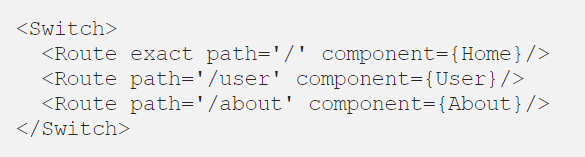
\includegraphics[width=11cm]{images/react-router.png}
\caption{Ví dụ React Router}
\label{fig:reactrouter}
\end{figure}

Hình \ref{fig:reactrouter} trên thể hiện cấu hình 
cơ bản của React Router với
đường dẫn (/path) và Route và giao diện tương ứng.

\subsubsection{Redux}
\paragraph{Khái quát về Redux}
Một ứng dụng web sẽ nhận dữ liệu từ phía máy chủ (back-end),
hay nhận những thao tác của người dùng (input, click, submit, …),
những thứ này chúng ta gọi đó là trạng thái (state) của ứng dụng.
Nếu biết được trạng thái của ứng dụng tại một thời điểm nào đó,
chúng ta sẽ biết vào thời điểm đó ứng dụng đã nhận dữ liệu nào,
những thao tác nào đã được người dùng truyền lên.

Ví dụ: Khi chúng ta click vào nút Back / Forward trên trình duyệt 
thì mỗi trang là một trạng thái của ứng dụng.

Như đã trình bày ở trên, ReactJS xây dựng lên các Single
Page Application, tức chỉ render một trang, và tất cả các
thành phần của ứng dụng sẽ được lưu trữ trong đó. Vì thế,
nếu ứng dụng phức tạp lên theo thời gian, các component sẽ nhiều
lên, và việc quản lý các state của chúng cũng ngày một lớn dần.
Giao diện ứng dụng (UI) cũng trở nên phức tạp vì chúng ta
cần quản lý các công việc active Routes, selected tabs, spinners,
pagination, … Trong ReactJS để truyền dữ liệu giữa các component anh
em, một state phải tồn tại (live) trong một component cha,
một phương thức (method) để update chính state này được cung cung
cấp bởi component cha, từ đây sẽ truyền xuống props của các
component con. Do vậy nếu một state phải được chia sẻ giữa các
component cách khá xa nhau trong một tree component thì state
này sẽ phải được truyền từ một component đến một component khác cho
đến khi nó đến được nơi mà nó được gọi.

\begin{figure}[H]
\centering
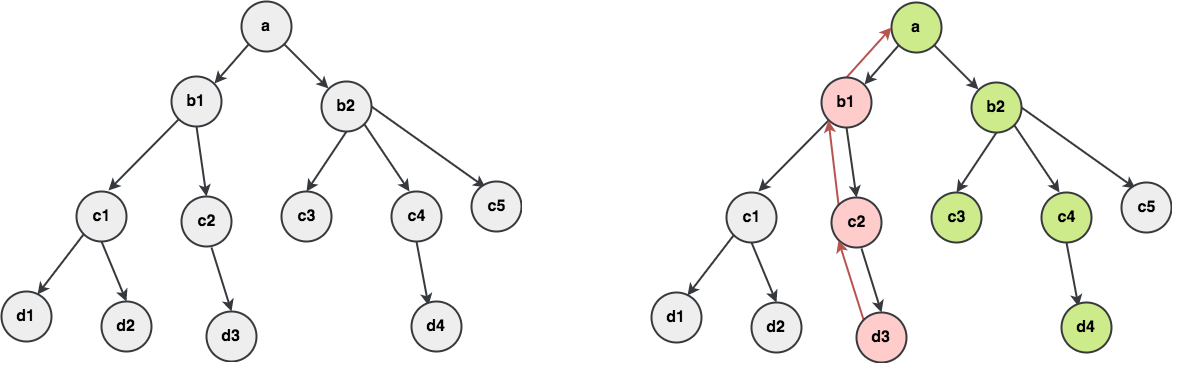
\includegraphics[width=16cm]{images/redux-state-transfer.png}
\caption{Truyền state giữa các component}
\end{figure}

Trong hình vẽ trên, giả sử nếu có một sự kiện ở node d3 kích
hoạt muốn thay đổi state d4 thì luồng dữ liệu sẽ được truyền
từ node d3 trở về node gốc là a, sau đó từ node a lại truyền data
đến các node con. Thứ tự truyền: d3 – c2 – b1 – a – b2 – c4 – d4.
Tương tự nếu muốn thay đổi state ở c3 thì thứ tự truyền là:
d3 – c2 – b1 – a – b2 – c3. Điều này làm cho bộ phận quản lý
state trong ứng dụng trở nên phức tạp và bừa bộn, do vậy ta
cần một công cụ quản lý trạng thái (state management tool)
như Redux. Giải pháp Redux đưa ra như sau:

\begin{figure}[H]
\centering
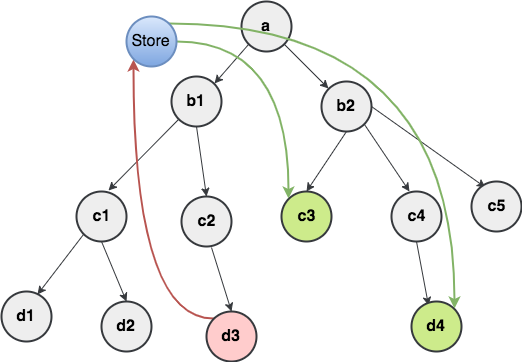
\includegraphics[width=10cm]{images/redux-solution.png}
\caption{Quản lý state trong Redux}
\end{figure}

Quay lại ví dụ ở trên thì ta cần map sự kiện từ node d3
về store của Redux rồi ở node d4, c3 cần connect với store
và cập nhật dữ liệu thay đổi.

\paragraph{Nguyên lý vận hành của Redux}
Cách Redux hoạt động khá đơn giản. Redux có một store lưu trữ
toàn bộ state của ứng dụng. Mỗi component có thể truy cập trực
tiếp đến state được lưu trữ thay vì phải truyền từ component
này qua component khác.

\begin{figure}[H]
\centering
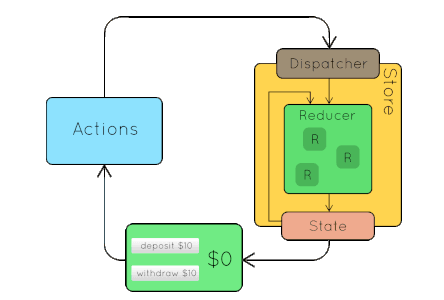
\includegraphics[width=12cm]{images/redux-without-middleware.png}
\caption{Kiến trúc của Redux}
\end{figure}

Redux có 3 thành phần là Action, Store và Reducer.

Action đơn giản là các sự kiện, mô tả những gì xảy ra như 
là cách mà chúng ta gửi dữ liệu từ ứng dụng đến Redux store, 
dữ liệu có thể đến từ sự tương tác của user và ứng dụng, 
API call hoặc khi submit một form, … Tuy nhiên action lại không 
chỉ rõ phần state nào thay đổi, việc này do Reducer đảm nhiệm. 
Reducer nhận vào một state cũ và action được gửi lên 
sau đó trả về một state mới. 

\begin{lstlisting}
(previousState, action) => newState
\end{lstlisting}

Những state này được lưu như những đối tượng (objects) và
chúng định rõ cách state của một ứng dụng thay đổi trong việc
phản hồi một action gửi đến store. Store là nơi lưu lại các
state của ứng dụng và nó là duy nhất
trong bất kì một ứng dụng Redux nào.

\paragraph{Middleware}
Một ứng dụng thực tế đòi hỏi có những thao tác xử lý cần thời
gian để phản hồi (các thao tác bất đồng bộ lấy dữ liệu từ
api hay các thao tác đọc ghi file hay đọc cookie từ trình duyệt, …),
các thao tác như vậy gọi là side effect. Để giải quyết được
các side effect này, trong Redux ta cần thực hiện nó ở middleware.

Trong Redux, Middleware cho phép chúng ta can thiệp vào giữa
thời điểm dispatch một action và thời điểm action đó đến được
reducer. Kiến trúc của Redux đầy đủ khi có middleware như hình dưới đây.

\begin{figure}[H]
\centering
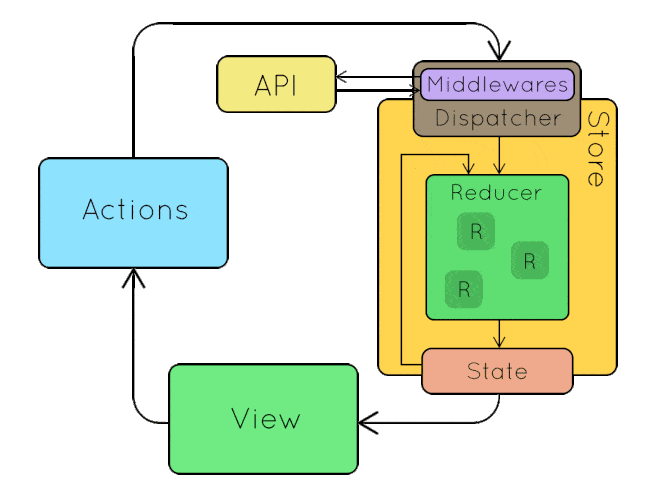
\includegraphics[width=12cm]{images/redux-architecture.png}
\caption{Kiến trúc của Redux với Middleware}
\end{figure}

Ta có thể tự viết một middleware hoặc có thể dùng những thư
viện middleware được xây dựng sẵn. Hiện tại có một vài thư viện
middleware cho Redux, ví dụ như redux-thunk, redux-saga,
redux-observable, … mỗi thư viện có phương pháp giải quyết
vấn đề side-effect riêng.
Trong project này sử dụng redux-saga để xử lý các side-effect.

\paragraph{Redux-saga}
Redux-saga là một thư viện hỗ trợ việc xử lý side-effect trong
ứng dụng React/Redux (ví dụ như xử lý bất đồng bộ khi load dữ liệu,…)
và làm cho các ứng dụng này trở nên đơn giản hơn.
Bằng cách sử dụng Generator Function, redux-saga giúp ta viết
code bất đồng bộ (async code) nhìn giống như là đồng bộ (synchronos).

Generator Function là function có khả năng hoãn lại quá trình
thực thi mà vẫn giữ nguyên được ngữ cảnh của function. Khác với
function bình thường là thực thi và trả về kết quả,
thì Generator function có thể thực thi, tạm dừng trả về
kết quả và thực thi tiếp (bằng cách sử dụng từ khóa \textbf{yield}).
Nếu như function bình thường khi được gọi sẽ thực thi hết tất cả
các câu lệnh trong hàm thì Generator function có khả năng tạm ngưng
trước khi hàm kết thúc và có thể tiếp tục chạy tại một thời điểm khác.
Chính chức năng này giúp ta giải quyết được vấn đề bất đồng bộ,
hàm sẽ dừng và đợi async chạy xong rồi tiếp tục thực thi.

\textit{Nguyên lý hoạt động của Redux-saga:} \\
Redux-saga cung cấp các hàm helper effect, các hàm này sẽ
trả về một effect object chứa các thông tin chỉ dẫn middleware
của Redux có thể thực hiện tiếp các hành động khác. Các hàm
helper effect sẽ được thực thi trong các generator function.
Ví dụ một số helper effect trong Redux-saga:
\begin{itemize}
\item \textit{takeEvery()}:
    thực thi và trả về kết quả của một action được gọi
\item \textit{takeLastest()}: nếu ta thực hiện một loạt các actions,
    nó sẽ chỉ thực thi và trả về kết quả của action cuối cùng.
\item \textit{put()}: dispatch một action.
\item \textit{call()}: gọi một function. Nếu nó trả về một Promise,
    sẽ tạm dừng saga cho đến khi Promise được giải quyết.
\end{itemize}
Ví dụ sử dụng helper effect trong Redux-saga:
\begin{lstlisting}[language=JavaScript,caption={Sử dụng Redux-Saga},captionpos=b]
// execute fetchPersonListSaga
// when action FETCH_PERSON_LIST is dispatched
yield takeEvery(FETCH_PERSON_LIST, fetchPersonListSaga);

// dispatch action pushSuccessNotification 
yield put(pushSuccessNotification(sequence, "Saved"));
\end{lstlisting}

% \subsubsection{Material-UI}
% \paragraph{Material Design}
% Material UI là một thư viện các React Component và được 
% tích hợp thêm cả Google’s Material Design. Trước tiên, 
% chúng ta sẽ tìm hiểu về nguyên lý Material Design. 

% Material Design là phong cách thiết kế áp dụng chủ yếu trong thiết
% kế ứng dụng Web, ứng dụng Mobile và đã trở thành một xu hướng
% phổ biến hiện nay. Đối với những Designer thiết kế UX/UI
% (giao diện / trải nghiệm người dùng), hay các lập trình viên
% front-end thì thuật ngữ Material Design không còn xa lạ.
% Có rất nhiều ứng dụng nổi tiếng thiết kế theo phong
% cách Material Design như các ứng dụng của Google
% (Google+, Gmail, Google Maps, …), Evernote, ePay, …

% \begin{figure}[H]
% \centering
% 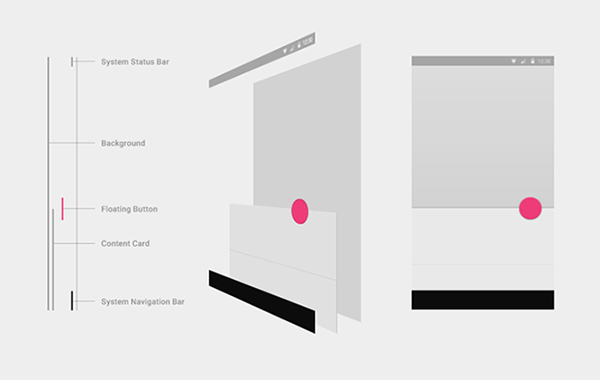
\includegraphics[width=14cm]{images/material-design.png}
% \caption{Thiết kế Material Design}
% \end{figure}

% Material Design là hình thức phát triển cao hơn của
% Flat Design (thiết kế phẳng), tuy nhiên thay vì cảm
% giác “phẳng lì” trên toàn bộ giao diện, Material Design là
% những lớp xếp chồng lên nhau, tạo chiều sâu, điểm nhấn hơn
% những thiết kế phẳng thông thường. Material Design chủ yếu tập
% trung vào những đường nét đơn giản, sử dụng những gam màu đậm,
% nổi bật, đồng thời cũng thường sử dụng những yếu tố đồ họa
% có cảm giác 3D, có hiệu ứng “nổi lên” (float) trên giao diện.
% Ngoài ra, thiết kế này còn bao gồm những chuyển động tự nhiên,
% tất cả những điều này đều nhằm mục đích mang lại cho người
% dùng trải nghiệm mới mẻ, thú vị và gần gũi hơn.

% Material Design có 3 yếu tố căn bản:
% \begin{itemize}[topsep=0ex]
% \item Thứ nhất là không gian: 
%     Không gian dưới lớp kính màn hình thiết bị được mô phỏng
%     như một không gian 3 chiều Oxyz với chiều sâu là trục Oz.
%     Để tạo chiều sâu cho thiết kế, designer cần điều chỉnh ánh
%     sáng một cách phù hợp.

% \begin{figure}[H]
% \centering
% 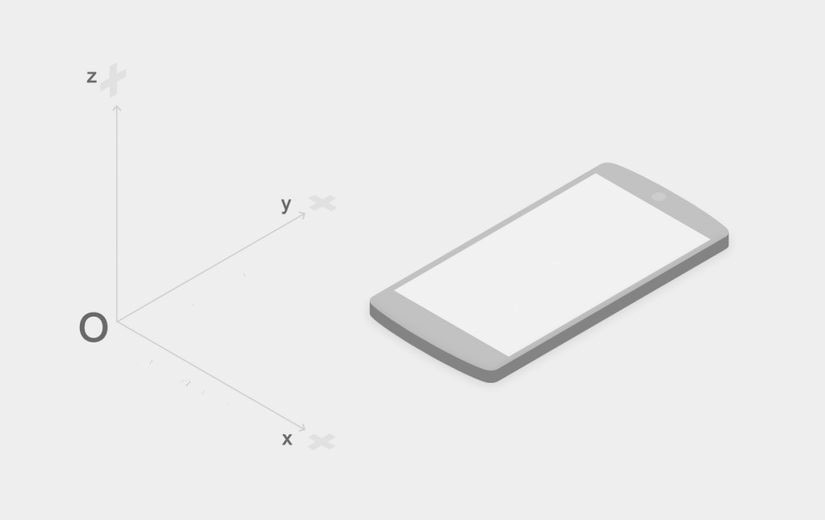
\includegraphics[width=12cm]{images/material-design-space.jpg}
% \caption{Material Design – Không gian}
% \end{figure}

% \item Thứ hai là ánh sáng:
%     Ánh sáng là yếu tố môi trường được sử dụng nhằm thể
%     hiện tính 3 chiều của không gian. Hệ quả của ánh sáng là hiệu ứng
%     đổ bóng (Drop Shadow), sẽ phân định vị trí các lớp Material trong
%     không gian theo trục Oz. Có hai loại nguồn sáng được kết hợp
%     là nguồn sáng chiếu trực tiếp và ánh sáng môi trường. Nguồn sáng
%     trực tiếp rất quan trọng, nó giống như nguồn sáng đèn pin,
%     nó mang lại hiệu ứng đổ bóng mạnh và sắc nét. Ánh sáng môi trường
%     thì nhẹ nhàng và không rõ nguồn, tạo viền bóng nhẹ xung quanh.
%     Thông thường, Material Design kết hợp cả hai nguồn sáng, mang
%     đến hiệu ứng bóng tổng hợp, mô phỏng không gian thực tế.

% \begin{figure}[H]
% \centering
% 
\includegraphics[width=14cm]{images/material-design-light.jpg}
% \caption{Material Design – Ánh sáng}
% \end{figure}

% \item Thứ ba là material (chất liệu): Là những mặt phẳng có độ dày
%     đồng nhất 1dp (1 in $\approx$ 160 dp) và nằm song song với mặt phẳng Oxy.
%     Các mặt phẳng Material sắp xếp chồng lên nhau theo trục Oz.
%     Thông qua việc thay đổi kích thước của bóng, ta sẽ dễ dàng
%     mô tả vị trí tương đối của mỗi lớp so với lớp khác.

% \begin{figure}[H]
% \centering
% 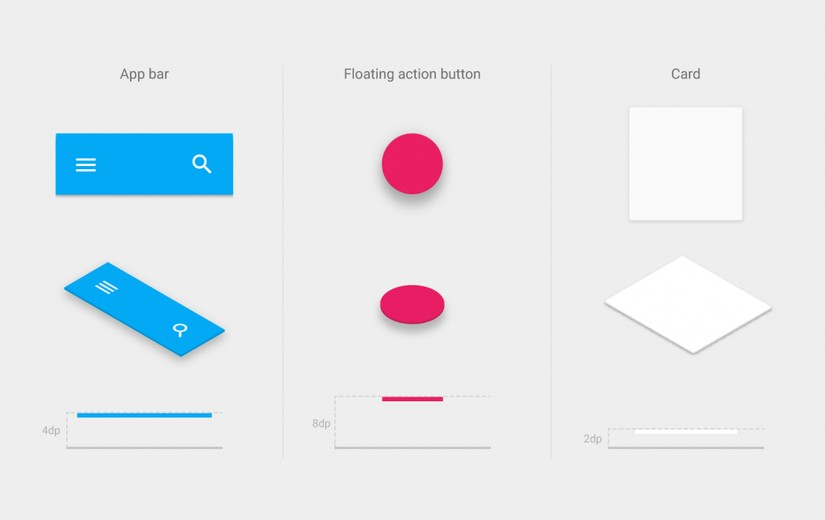
\includegraphics[width=14cm]{images/material-design-material.png}
% \caption{Material Design – Chất liệu}
% \end{figure}

% \end{itemize}

% Để có một thiết kế ấn tượng với Material Design cần
% chú ý một vài hiệu ứng và chi tiết:
% \begin{itemize}[topsep=0ex]
% \item Hiệu ứng tự nhiên: ví dụ khi bạn nhấn chọn một thành phần,
%     hiệu ứng sóng trên màn hình sẽ tỏa ra tự vị trí ngón tay
%     bạn chứ không phải từ một hướng cố định.

% \item Hiệu ứng bề mặt: khi chuyển trang, các thành phần phải chuyển
%     động một cách tự nhiên và liên tục chứ không biến mất

% \item Có thứ tự: những thành phần ở sau sẽ xuất hiện trước,
%     thành phần lớn hơn sẽ xuất hiện trước, thành phần quan trọng
%     hơn sẽ xuất hiện trước.

% \item Thống nhất: chuyển động của những Material phải thống nhất
%     từ cùng một hướng, tạo sự đồng đều cho tổng thiết kế.
% \end{itemize}

% \paragraph{Material-UI}
% Như đã trình bày ở trên, Material UI là một thư viện các
% React component tích hợp thêm Google’s Material Design.
% Material UI cung cấp khá đầy đủ các component để có thể tạo
% ra một trang web một cách nhanh chóng hơn mà không phải ngồi
% chỉnh CSS từng chút một.

% Ví dụ để tạo ra các nút bấm như hình dưới,
% ta chỉ việc sử dụng Button component mà Material UI cung cấp.
% \begin{figure}[H]
% \centering
% 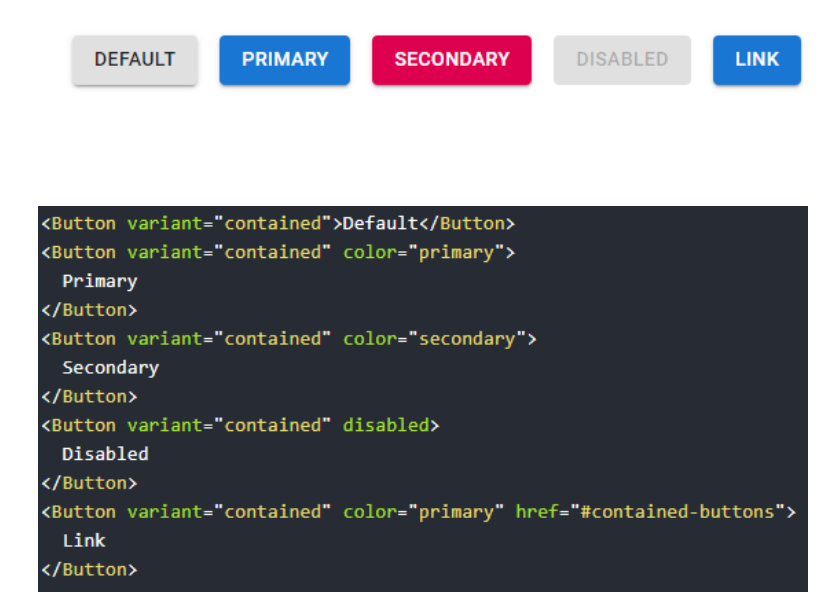
\includegraphics[width=14cm]{images/material-ui-button.png}
% \caption{Material UI – Button}
% \end{figure}

% Việc thêm màu sắc là vô cùng đơn giản với những thuộc
% tính được định nghĩa sẵn, màu sắc là chuẩn theo thiết
% kế Material Design. 
% Với Material UI, chúng ta còn dễ dàng chia bố cục và
% responsive trang web. Grid component sẽ chia màn hình theo
% bố cục 12 cột, 5 loại màn hình theo
% kích cỡ (xs, sm, md, lg, xl).

% Cùng một nội dung nhưng khi được hiển thị trên các màn
% hình khác nhau sẽ hiển thị theo cách khác nhau, đảm bảo sự thuận
% tiện nhất cho người dùng.  Thuật ngữ “Responsive Design” ám
% chỉ cách thiết kế trang web hiển thị tương thích với mọi kích thước
% thiết bị, tức là bố cục trang web sẽ tự đáp ứng theo hành vi
% người dùng và môi trường hiển thị. Môi trường này chính là kích thước
% của trình duyệt, kích thước hoặc hướng xoay thiết bị. Thiết
% kế Responsive không chỉ giúp cho người dùng có một trải nghiệm thú
% vị hơn khi truy cập website, mà còn giúp chủ sở hữu dễ dàng
% quản lý các trang web của mình hơn.

% Ngoài ra Material UI cũng có sẵn kho Icon khổng lồ trên đầy
% đủ các lĩnh vực giúp chúng ta dễ dàng chọn ra icon đẹp và
% phù hợp nhất với mỗi nội dung trên trang web.


\subsection{Công nghệ lưu trữ - Redis}
Redis~\cite{redis:online} là viết tắt của Remote Dictionary Server
(máy chủ từ điển từ xa), lưu trữ dữ liệu dưới dạng
KEY-VALUE trong bộ nhớ. Là phần mềm mã nguồn mở có tốc độ
truy cập nhanh để dùng làm cơ sở dữ liệu đơn giản, bộ nhớ đệm (cache),
trình chuyển tiếp (broker) tin nhắn hoặc
được sử dụng làm danh sách tác vụ chờ xử lý (queue). 

Redis hiện cung cấp thời gian phản hồi ở tốc độ chưa đến
một mili giây, giúp thực hiện hàng triệu yêu cầu mỗi giây cho
các ứng dụng thời gian thực trong lĩnh vực Trò chơi, Quảng cáo, Dịch
vụ tài chính, Chăm sóc sức khoe, IoT, … Cụ thể, Redis thường được chọn
sử dụng cho các hoạt động lưu trữ bộ nhớ đệm, quản lý phiên, trò chơi,
bảng xếp hạng, phân tích thời gian thực, dữ liệu không gian
địa lý, ứng dụng đặt xe, trò chuyện / nhắn tin, phát trực tiếp
nội dung đa phương tiện, …

Redis là một cơ sở dữ liệu NoSQL. NoSQL là một dạng cơ sở dữ liệu
phi quan hệ, sử dụng nhiều loại mô hình dữ liệu đa dạng để
truy cập và quản lý dữ liệu trong bộ nhớ và tìm kiếm, NoSQL được
tối ưu hóa dành riêng cho các ứng dụng yêu cầu mô hình dữ liệu
linh hoạt có lượng dữ liệu lớn và độ trễ thấp, đạt được bằng cách
giảm bớt một số hạn chế về tính nhất quán của dữ liệu.

\begin{figure}[H]
    \centering
    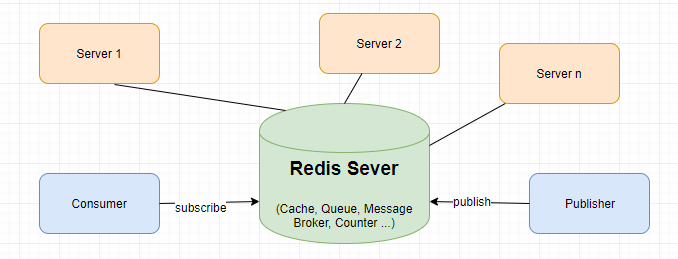
\includegraphics[width=14cm]{images/redis.png}
    \caption{Redis server}
\end{figure}

\textit{Cách thức hoạt động của Redis:}

Toàn bộ dữ liệu của Redis nằm trong bộ nhớ (RAM), khác với những loại 
cơ sở dữ liệu thông thường khác lưu dữ liệu trên ổ đĩa hoặc ổ SSD. 
Phần lớn các tác vụ trên cơ sở dữ liệu truyền thống đều yêu cầu 
truy cập qua lại tới ổ đĩa, do vậy sẽ tốn thời gian tìm kiếm, 
dữ liệu của Redis nằm trên RAM nên sẽ không mất thời gian này. 
Do đó Redis có thể hỗ trợ thêm khá nhiều tác vụ và có thời gian 
phản hồi nhanh hơn. Hiệu suất của Redis rất tốt với các tác 
vụ đọc ghi thông thường mất chưa đầy một mili giây và hỗ trợ 
hàng triệu tác vụ mỗi giây. 

Khác với các cơ sở dữ liệu quan hệ như MySQL hay PostgreSQL,
Redis không có bảng. Redis lưu dữ liệu dưới dạng KEY-VALUE và hỗ
trợ nhiều cấu trúc dữ liệu cơ bản như hash, list, set,
sorted set, string, … Bên cạnh đó Redis có 2 background threads chuyên
làm nhiệm vụ định kì ghi dữ liệu trên đĩa cứng, cơ chế backup
này giúp cho Redis có độ bảo mật và sửa lỗi cao.

\textit{Một số ứng dụng phổ biến của Redis:}
\begin{itemize}[topsep=0ex]
\item Lưu trữ bộ nhớ đệm (caching): Sử dụng bộ nhớ đệm để giảm độ trễ
    khi truy cập dữ liệu, tăng năng suất và giảm tải cho cơ sở dữ
    liệu và ứng dụng của bạn. Redis có thể phục vụ những dữ liệu thường
    xuyên được yêu cầu với thời gian phản hồi chưa đến một mili giây
    và cho phép dễ dàng thay đổi quy mô nhằm đáp ứng mức tải cao hơn
    mà không cần tốn kém chi phí vào back-end.

\item Bảng xếp hạng game: Redis là giải pháp hay được các nhà phát
    triển game dùng để xây dựng bảng xếp hạng theo thời gian thực
    (real-time leaderboard). Sử dụng cấu trúc dữ liệu Sorted Set của
    Redis, cấu trúc dữ liệu này đảm bảo tính duy nhất của các thành
    phần trong khi vẫn duy trì danh sách được sắp xếp theo điểm số
    của người dùng. Danh sách cập nhật mỗi khi điểm số người dùng thay đổi.

\begin{figure}[H]
    \centering
    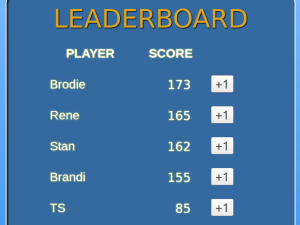
\includegraphics[width=10cm]{images/real-time-leader-board.png}
    \caption{Ứng dụng Redis trong bảng xếp hạng game}
\end{figure}

\item Lưu trữ phiên (session): Các nhà phát triển ứng dụng thường sử
    dụng Redis để lưu trữ, quản lý phiên cho các ứng dụng quy mô
    Internet. Quản lý dữ liệu phiên chẳng hạn như hồ sơ người dùng,
    thông tin xác thực đăng nhập (token), trạng thái phiên, …

\item Trò chuyện, nhắn tin, hàng chờ xử lý tác vụ: Redis hỗ trợ Pub/Sub
    (là cấu trúc gửi – nhận tin nhắn mà người gửi và người nhận không
    biết nhau) với nhiều cấu trúc dữ liệu như list, sorted set, hash.
    Điều này cho phép Redis hỗ trợ những chat rooms hiệu năng cao,
    luồng tin nhắn theo thời gian thực.
\end{itemize}

\textit{So sánh Redis và một loại cơ sở dữ liệu quan hệ thông thường (MySQL)}
\begin{table}[H]
\centering
\begin{tabular}{| m{3cm} | m{6cm} | m{6cm} |}
\hline
& \textbf{Redis} & \textbf{MySQL} \\ 

\hline
\multirow{5}{3cm}{Cấu trúc cơ sở dữ liệu} &
Lưu trữ dạng KEY-VALUE & Lưu trữ dạng bảng \\  
\cline{2-3}
& Lưu dữ liệu trong RAM, là máy chủ cấu trúc dữ
liệu vì các key có thể chứa string, hash, list,
set và sorted set
& MySQL cung cấp một máy chủ cơ sở dữ liệu quan hệ SQL
rất nhanh, đa luồng, đa người dùng, mạnh mẽ \\  

\hline
\multirow{9}{3cm}{Ưu điểm}
& $\bullet$ Dễ cài đặt, sử dụng, deploy, maintain, … & 
$\bullet$ Cơ sở dữ liệu quan hệ mã nguồn mở được sử dụng rộng rãi \\
& $\bullet$ Lưu trữ dữ liệu trong bộ nhớ nên cho hiệu
    năng cao và tốc độ nhanh &
$\bullet$ Dễ sử dụng, khả năng tương thích cao, hỗ trợ đa nền tảng,
cộng đồng phát triển mạnh mẽ \\
& $\bullet$ Mã nguồn mở, ổn định, chi phí hiệu quả &
$\bullet$ Hỗ trợ index và full-text searching \\
& $\bullet$ Khả năng mở rộng cao, hỗ trợ sao lưu vào đĩa cứng & \\
& $\bullet$ Cấu trúc dữ liệu đa dạng & \\
\hline
\multirow{5}{3cm}{Trường hợp nên sử dụng} & 
$\bullet$ Có dữ liệu dạng KEY-VALUE & $\bullet$ Cần cơ sở dữ liệu quan hệ \\
& $\bullet$ Cần lưu cache & $\bullet$ Khi có các hoạt động phân tán \\
& $\bullet$ Cần hiệu năng cao &
$\bullet$ Cần bảo mật cao và hoạt động đơn giản \\
& $\bullet$ Kích thước dữ liệu ổn định &
$\bullet$ Không sử dụng khi dữ liệu lớn dần và 
không thể cache hết lên bộ nhớ \\
\hline
\multirow{3}{3cm}{Nhược điểm} & 
$\bullet$ Redis sử dụng RAM nên khi lượng file cache lớn sẽ
dẫn đến thiếu RAM cho server &
$\bullet$ Nhiều vấn đề về lưu trữ procedure và trigger \\
& $\bullet$ Không thể truy vấn trực tiếp các object & \\
\hline
\end{tabular}
\caption{So sánh Redis và MySQL}
\end{table}

\subsection{Công nghệ lưu trữ - PostgreSQL}

\subsubsection{Tổng quan về PostgreSQL}
PostgreSQL, còn được gọi là Postgres, là một hệ thống quản lý cơ sở 
dữ liệu quan hệ miễn phí mã nguồn mở chú trọng vào tính mở rộng và 
tính tương thích với chuẩn SQL. Ban đầu có tên là POSTGRES, có nguồn
gốc từ cơ sở dữ liệu Ingress được phát triển tại

Đại học California, Berkeley. Vào năm 1996, dự án được đổi tên thành
PostgreSQL. PostgreSQL được viết bằng ngôn ngữ C và có thể chạy trên nhiều
hệ điều hành như Linux, macOS, Windows, \ldots Đồng thời hỗ trợ các tính
năng tương tự như nhiều các cơ sở dữ liệu quan hệ khác.
Phiên bản PostgreSQL sử dụng trong đồ án này là 11.8.

\subsubsection{Tổng quan về Index}
Index trong cơ sở dữ liệu là một cấu trúc dữ liệu giúp cải thiện
tốc độ truy vấn dữ liệu trên các bảng với đánh đổi là sử dụng thêm
không gian lưu trữ nhằm duy trì cấu trúc dữ liệu index cũng như
làm tăng thời gian ghi dữ liệu. Index được sử dụng để nhanh chóng
định vị dữ liệu mà không phải tìm duyệt qua toàn bộ các hàng trong
bảng của cơ sở dữ liệu mỗi khi bảng đó được truy cập. Index có thể
được tạo sử dụng một hay nhiều cột trong cùng một bảng, cung cấp
cơ chế tăng tốc quá trình tra cứu ngẫu nhiên và truy cập có thứ
tự các bản ghi trong cơ sở dữ liệu. 

Index được chia làm hai loại kiến trúc:
Clustered Index và Non-clustered Index.

Với clustered index, các hàng trong cơ sở dữ liệu được lưu trữ
trên đĩa theo cùng thứ tự với index. Do đó mỗi bảng chỉ tồn tại
duy nhất một clustered index. Với non-clustered index thì cấu trúc dữ
liệu index là cấu trúc dữ liệu nằm ngoài bảng, các hàng trong bảng
không được đảm bảo thứ tự giống như thứ tự của index. Một bảng có
thể có rất nhiều non-clustered index. Thông thường với truy cập trên
clustered index sẽ nhanh hơn trên non-clustered index vì dữ liệu
sẽ không bị phân mảnh ở nhiều vị trí trong ổ cứng.

\subsubsection{Index trong PostgreSQL}
Trong PostgreSQL, clustered index không được hỗ trợ. Tuy nhiên
PostgreSQL lại hỗ trợ nhiều kiểu index như B-Tree, Hash, GiST,
SP-GiST, GIN và BRIN. Mỗi một kiểu index sử dụng một thuật toán
riêng biệt để tối ưu cho nhiều loại câu truy vấn khác nhau.
Mặc định khi sử dụng lệnh CREATE INDEX thì index B-Tree sẽ được tạo,
index này cũng phù hợp với hầu hết các
trường hợp truy vấn~\cite{postgresdocs}.

Index kiểu B-Tree có thể được xử dụng cho các câu truy vấn
liên quan đến tìm kiếm bằng, tìm kiếm khoảng hoặc trong trường
hợp dữ liệu được sắp xếp theo một trường nào đó. Trình lập kế hoạch
cho các truy vấn của PostgreSQL sẽ xem xét sử dụng index B-Tree
bất kì khi nào trường mà có index nằm trong một trong
các phép toán so sánh như $<$ $<=$ $=$ $>=$ $>$.

Các toán tử tương đương hoặc tổ hợp của chúng, như là phép toán
BETWEEN và IN, cũng có thể sử dụng được index B-Tree.
Ngoài ra các phép toán liên quan đến NULL như IS NULL hay
IS NOT NULL cũng có thể được tăng tốc bằng index B-Tree.

Trình tối ưu cũng có thể sử dụng index B-Tree cho các câu
truy vấn sử dụng toán tử pattern matching như LIKE và ~
nếu mà pattern được sử dụng bắt đầu là một xâu hằng số
như ‘foo\%’ nhưng không phải là ‘\%bar’. 

B-Tree có thể cũng được sử dụng để lấy dữ liệu được sắp
xếp theo thứ tự của cột được index.

Index kiểu Hash chỉ có thể được sử dụng trong các câu truy
vấn sử dụng toán tử so sánh bằng. Để tạo index Hash trong PostgreSQL,
ta sử dụng:
\begin{lstlisting}[caption={Tạo index sử dụng Hash}, captionpos=b]
CREATE INDEX name ON table USING HASH (column);
\end{lstlisting}

\subsubsection{Full Text Search trên PostgreSQL}
\paragraph{Cơ bản về Full Text Search}
Các toán tử tìm kiếm text trên các CSDL quan hệ đã tồn
tại từ rất lâu như LIKE hay ILIKE. Nhưng những toán tử đó thiếu
đi những tính chất mà cần có trong các hệ thống thông tin hiện đại như:
\begin{itemize}[topsep=0ex]
\item Hỗ trợ ngôn ngữ, thậm chí với cả tiếng Anh. Các toán tử
    trên không phù hợp cho việc xử lý những từ gần giống nghĩa hoặc
    được suy diễn, như satisfy và satisfies trong tiếng Anh. Có thể
    dùng toán tử logic OR để tìm kiếm cả 2 nhưng phải liệt kê rất
    nhiều trường hợp và một số từ có thể có rất nhiều từ
    được suy diễn hoặc gần nghĩa.

\item Không hỗ trợ xếp hạng (ranking) trên tập kết quả,
    dẫn đến tìm kiếm không hiệu quả khi mà có thể có tới rất
    nhiều document được tìm thấy trong một câu truy vấn.

\item Các phép toán đó thường chậm vì không hỗ trợ đánh chỉ
    số, mỗi một câu truy vấn phải duyệt qua toàn bộ các document.
\end{itemize}

PostgreSQL hỗ trợ tiền xử lý các document và đánh chỉ
số để tăng tốc các câu truy vấn. Tiền xử lý document bao gồm việc:
\begin{itemize}[topsep=0ex]
\item Phân tích document thành các token.
\item Chuyển các token thành các lexeme.
\item Lưu trữ các dữ liệu sau khi tiền xử lý
    document để tối ưu cho truy vấn.
\end{itemize}

Một document trong PostgeSQL thông thường là một cột chứa
xâu của bảng CSDL, hoặc có thể là một 
tổ hợp (thông qua phép ghép nối xâu) của những trường
đó trong một bảng hay trong nhiều bảng hoặc
có thể được truyền từ ngoài vào. 

Một token là một xâu biểu diễn một từ được phân tích ra từ document.

Một lexeme cũng là một xâu, tương tự như token, nhưng đã
được chuẩn hóa (normalize) sao cho những dạng khác nhau của
một từ trở thành giống nhau. Việc chuẩn hóa luôn luôn
thực hiện chuyển tất cả các kí tự thành lower-case, và thông
thường có cắt bỏ một vài các hậu tố như e hoặc es trong tiếng
Anh. Đồng thời ở bước chuyển từ token thành càng lexeme cũng
thông thường loại bỏ những stop word, là những từ rất phổ biến
trở thành vô nghĩa khi tìm kiếm, PostgreSQL sử dụng Dictionary
để thực thi bước này.

Dictionary trong PostgreSQL cho phép hiệu chỉnh quá trình
chuẩn hóa thành lexeme, bao gồm:
\begin{itemize}[topsep=0ex]
\item Định nghĩa các stop word được loại bỏ.
\item Ánh xạ các từ đồng nghĩa thành một từ.
\item Ánh xạ cụm từ thành một từ.
\item Ánh xạ các biến thể của một từ thành dạng chuẩn.
\end{itemize}

PostgreSQL sử dụng kiểu dữ liệu tsvector để lưu trữ dữ
liệu sau khi tiền xử lý document, đồng thời sử dụng kiểu
tsquery để biểu diễn các câu truy vấn.

Để chuyển từ một xâu sang kiểu tsvector ta sử dụng hàm
to\_tsvector. Còn để chuyển một xâu bất kì sang một tsquery,
ta sử dụng plainto\_tsquery. 

Để thực hiện Full Text Search một tsvector với một tsquery,
ta sử dụng toán tử @@.

\paragraph{Full Text Search cho tiếng Việt}
Để thực hiện Full Text Search với tiếng Việt,
trong đồ án này sử dụng một hàm được định nghĩa bằng SQL như sau: 
\begin{figure}[H]
\centering
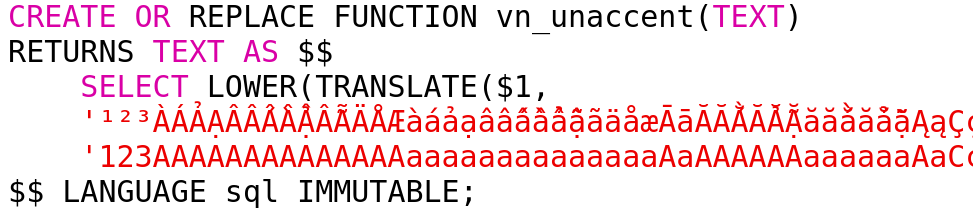
\includegraphics[width=10cm]{images/unaccent.png}
\end{figure}
Khi đó, thay vì sử dụng trực tiếp to\_tsvector và plainto\_tsquery,
ta sử dụng \\
to\_tsvector(vn\_unaccent(text)) và plainto\_tsquery(vn\_unaccent(text)).

\paragraph{Đánh chỉ số cho Full Text Search}
Để sử dụng Index cho Full Text Search, trước tiên ta cần tạo
một cột trong CSDL lưu trữ kiểu dữ liệu tsvector.
Có hai loại Index hay được sử dụng cho Full Text Search là GIN và GiST. 

\noindent Để Index sử dụng GIN, cú pháp như sau:
\begin{lstlisting}[caption={Tạo index sử dụng GIN},captionpos=b]
CREATE INDEX idx_textsearch ON sometable USING GIN (tsvector_column);
\end{lstlisting}

\noindent Còn nếu sử dụng GiST:
\begin{lstlisting}[caption={Tạo index sử dụng GiST},captionpos=b]
CREATE INDEX idx_textsearch ON sometable USING GIST (tsvector_column);
\end{lstlisting}

Khi đó toán tử @@ có thể sử dụng Index để
tăng tốc câu truy vấn. Trong PostgreSQL, Index Full Text Search
thông thường sử dụng GIN hơn sử dụng GiST. 

Thông thường sẽ sử dụng trigger để cập nhật các trường
tsvector trong CSDL khi chèn hoặc chỉnh sửa.

\paragraph{GIN}
\begin{figure}[H]
\centering
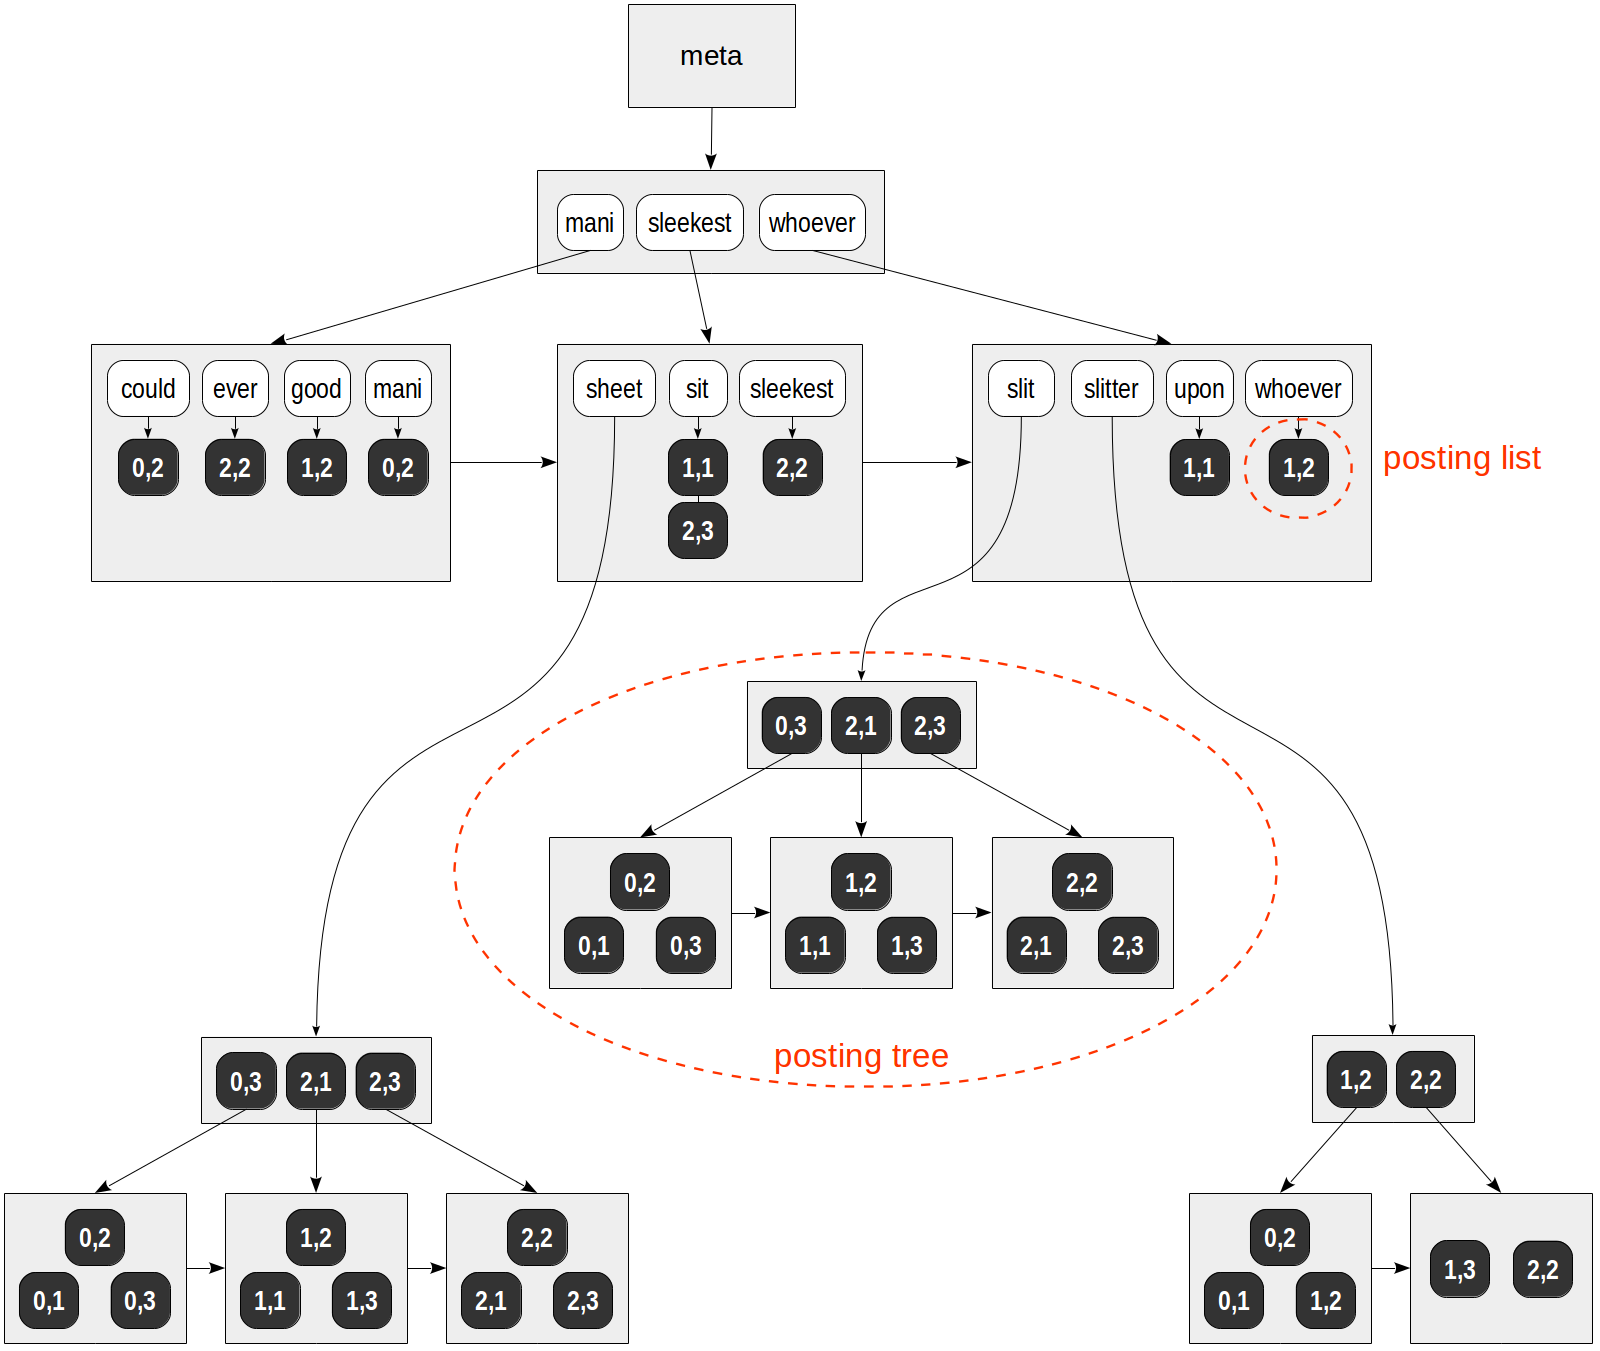
\includegraphics[width=13cm]{images/GIN.png}
\caption{Cấu trúc của GIN}
\end{figure}

GIN là viết tắt của Generalized Inverted Index. GIN được thiết
kế cho việc đánh chỉ số những giá trị tổng hợp (composite value),
và cho phép tìm kiếm cho các phần tử xuất hiện
trong các compostive value. 

Nếu quy ước một composite value là một item, còn phần tử trong
composite value là một key thì GIN 
luôn luôn lưu trữ và tìm kiếm trên key chứ không phải trên item.
Một GIN index lưu trữ tập các cặp (key, posting list) trong đó
posting list là tập các ID của các hàng trong bảng của CSDL.
Một ID có thể được nằm trong nhiều các posting list vì một
item có thể có nhiều các key. Mỗi một key được lưu trữ một
lần duy nhất, do đó nên GIN rất phù hợp trong trường hợp một
key xuất hiện nhiều lần. posting list được lưu với thứ tự
từ nhỏ đến lớn các ID của các hàng. Nếu posting list quá lớn
sẽ được chuyển thành posting tree, cấu trúc tương tự như B-Tree. 

\subsection{Công nghệ back-end}
\subsubsection{Giới thiệu về ngôn ngữ Go}
Go là ngôn ngữ biên dịch kiểu tĩnh được tạo ra tại Google.
Cú pháp của Go tương tự như của ngôn ngữ C, đồng thời cũng
bị ảnh hưởng lớn bởi ngôn ngữ này. Ngôn ngữ Go cũng thông
thường được gọi với tên là Golang.
Sau đây là một số đặc điểm của ngôn ngữ Go:
\begin{itemize}[topsep=0ex]
\item Cú pháp và môi trường lập trình của Go có
    tính tương đồng với các ngôn ngữ lập trình
    kiểu động (dynamic language) như:
    \begin{itemize}[topsep=0ex]
    \item Rút gọi khai báo biến, không cần phải khai báo kiểu
        thông qua cơ chế type inference.
    \item Biên dịch nhanh.
    \item Quản lý các gói thư viện từ xa và các
        package có document truy cập online.
    \end{itemize}

\item Sử dụng cách tiếp cận đặc biệt với một số vấn đề:
    \begin{itemize}[topsep=0ex]
    \item Xây dựng sẵn trong ngôn ngữ một số cơ chế cho lập trình
        đồng bộ như: tiến trình nhẹ (light-weight process,
        hay còn gọi là goroutine), channel và câu lệnh select.
    \item Toolchain mặc định khi biên dịch sinh ra file thực
        thi sẽ không chứa phụ thuộc ngoài.
    \end{itemize}

\item Ngôn ngữ được thiết kế đủ đơn giản để lập trình
    viên có thể dễ dàng hiểu và ghi nhớ.
\end{itemize}

\subsubsection{Goroutine, Chanel và khối lệnh Select}
Ngôn ngữ Go được xây dựng sẵn trong ngôn ngữ những cơ chế hỗ trợ việc
lập trình đồng bộ. Đồng bộ ở đây không chỉ là song song ở mức CPU mà
đồng thời cả việc sử dụng Asynchronous I/O cho phép các câu lệnh như
truy cập database hay đọc gói tin từ mạng chạy trong khi tiến
trình vẫn được sử dụng cho công việc khác. Kỹ thuật này phổ biến
trong các server mà sử dụng event-based.

Trung tập của xây dựng chương trình đồng bộ trong Go là tiến trình
nhẹ (light-weight process) gọi là Goroutine. Một lời gọi hàm mà
được đặt sau từ khóa go sẽ bắt đầu hàm đó trong một Goroutine mới.
Trong đặc tả ngôn ngữ (Language Specfication) không chỉ định Goroutine
được cài đặt như nào nhưng với cài đặt hiện tại thì các Goroutine
sẽ được phân bố vào một tập nhỏ các luồng ở mức hệ điều hành,
tương tự như cơ chế phân phát tiến trình trong ngôn ngữ Erlang.
Khi chương trình Go mới bắt đầu sẽ chứa duy nhất
một goroutine gọi là main goroutine.

Chương trình viết bằng Go sẽ thường sử dụng Channel, một cơ chế để
gửi các thông điệp (Message) giữa các goroutine. Channel trong Go có thể
có chứa Buffer hoặc không. Nếu không chứa Buffer thì Channel mỗi một
thời điểm chỉ chứa tối đa một Message, các lời gọi gửi message vào
channel tiếp theo đó sẽ bị block. Nếu chứa Buffer thì kích thước
của buffer cũng bị giới hạn, các message được lưu trữ và truy xuất theo
cơ chế FIFO. Khi đọc từ một channel mà channel chưa chứa message nào
cả thì goroutine đọc từ channel đó sẽ bị block. 

Channel trong Go có chứa kiểu tĩnh, nghĩa là một channel có kiểu
là chan T sẽ chỉ có thể gửi và nhận message thuộc kiểu T.
Go có chứa cú pháp đặc biệt để tương tác với channel:
\begin{itemize}[topsep=0ex]
\item \textit{x <- ch} để đọc từ channel ch vào biến x.
\item \textit{ch <- x} để gửi message x vào channel ch.
\end{itemize}
Trong trường hợp tương tác với nhiều lệnh nhận hoặc gửi message với các
channel, chương trình Go có thể sử dụng khối lệnh select để lựa chọn
lệnh nhận/gửi đầu tiên mà kết thúc block trên các channel. Cú pháp
của khối lệnh select trong Go tương tự với switch nhưng khác
là mỗi một nhãn case trong khối lệnh select sẽ là một
lệnh tương tác với channel.

\subsubsection{Các công cụ tích hợp}
Bản cài đặt bộ công cụ của Go bao gồm nhiều các công cụ
lên quan đến xây dựng, kiểm thử và phân tích code, gồm:
\begin{itemize}[topsep=0ex]
\item \textbf{go build}, để xuất file nhị phân từ các file mã nguồn.
\item \textbf{go test}, dùng để chạy các unit test và các benchmark.
\item \textbf{go fmt}, dùng để format code.
\item \textbf{go get}, tải xuống và cài đặt các thư viện và
    các file thực thi đi kèm. 
\item \textbf{go vet}, một static analyzer cho việc tìm kiếm
    các vị trí có thể có lỗi trong code. 
\item \textbf{go run}, một shortcut cho phép biên dịch
    và chạy chương trình. 
\item \textbf{go doc}, dùng để hiển thị document của thư viện. 
\item \textbf{go mod}, dùng để quản lý module - xuất hiện từ
    phiên bản Go 1.11. 
\item \textbf{go generate}, dùng để gọi code generator.
\end{itemize}

\subsection{Docker}
\subsubsection{Công nghệ container}
Công nghệ container được sinh ra có mục đích tương tự như công
nghệ máy ảo (Virtual Machine)~\cite{dockerbook}.
Điểm khác biệt lớn nhất là mỗi container
sẽ không yêu cầu phải chạy một hệ điều hành đầy đủ và riêng biệt.
Tất cả các container trên một máy chủ đều chia sẻ chung một hệ
điều hành. Chính điểm khác biệt này làm cho container sử dụng ít tài
nguyên CPU, RAM và bộ nhớ lưu trữ hơn VM rất nhiều dẫn đến tiết
kiệm chi phí cho việc chạy server, vá lỗi hệ điều hành và các
vấn đề bảo trì hệ thống khác.

Công nghệ Container hiện đại được bắt đầu từ hệ điều hành Linux.
Một số các công nghệ của nhân Linux giúp tạo nên sự phát triển của
công nghệ container bao gồm: kernel namespace, control group, union
filesystem. Dù cho các công nghệ này đã tồn tại từ lâu những để
sử dụng nó thì rất phức tạp và ngoài tầm với của phần lớn các
công ty công nghệ. Sự thay đổi bắt đầu khi Docker được tạo ra
giúp đơn giản hóa rất nhiều quá trình tạo và quản lý các container. 

Docker ban đầu được tạo nên chỉ để chạy trên môi trường Linux.
Tuy nhiên, trong một vài năm gần đây, Microsoft đã phát triển
công nghệ container trên hệ điều hành Windows 10 và Windows Server từ
đó giúp việc sử dụng Docker trên Windows tương tự như trên Linux.
Nhưng bởi vì container sẽ chia sẻ hệ điều hành với hệ điều hành
mà Docker chạy trên (được gọi là host), từ đó dẫn đến một container
dùng Linux sẽ không thể chạy trên Windows và ngược lại.

\subsubsection{Sơ lược về Docker}
Docker được bắt đầu phát triển bởi Docker, Inc vào năm 2013,
bao gồm các thành phần:
\begin{itemize}[topsep=0ex]
\item Software: gồm một chương trình chạy ngầm (daemon) gọi là dockerd,
    là chương trình quản lý các container và xử lý các container object.
    Daemon dockerd lắng nghe các yêu cầu từ bên ngoài gửi đến thông qua
    Docker Engine API. Đi kèm là một chương trình client, gọi là docker,
    cung cấp một giao diện dòng lệnh giúp tương tác với daemon dockerd.

\item Object: các Docker Object là các thực thể cấu thành lên một
    ứng dụng chạy trên Docker. Các Docker object được chia thành ba
    loại là image, container và service.
    \begin{itemize}
    \item Một Docker image là một tập các file chỉ đọc dùng làm
        template để tạo nên các container. Các image được dùng để
        lưu trữ và triển khai các ứng dụng.

    \item Một Docker container là một môi trường được đóng gói
        và chuẩn hóa để chạy ứng dụng.

    \item Một Docker service là một thực thể dùng để chạy nhiều
        container trên nhiều máy trong một cluster. Tập các máy chạy
        Docker trong một cluster gọi là một Swarm.  
    \end{itemize}
\end{itemize}

\subsubsection{Dockerfile}
Để xây dựng các image cho việc đóng gói ứng dụng, ta có thể
chạy container, cài đặt các file cần thiết và sử dụng lệnh
\textbf{docker commit} để lưu container thành image. Tuy nhiên thông thường
việc tạo image thông qua việc sử dụng Dockerfile.

Dockerfile là một file văn bản có chứa những instruction(chỉ thị) để xây
dựng một image. Trong đó có các lệnh như: chỉ định image gốc nào mà
sẽ được xây dựng lên, chỉ định lệnh nào được chạy khi bắt đầu
một container, chỉ định những file hay thư mục nào được sao
chép từ host vào container, ...
. Để xây dựng lên image bằng Dockerfile, ta sử dụng docker build.

Ví dụ trong đồ án này sử dụng Dockerfile sau để
xây dựng lên Webserver viết bằng Go:

\begin{lstlisting}[caption={Xây dựng image của back-end server},captionpos=b]
FROM golang:1.14.3-alpine3.11 as builder
WORKDIR /go/baseweb/
COPY . .
RUN go build

FROM alpine:3.11
WORKDIR /go/
COPY --from=builder /go/baseweb/baseweb .
EXPOSE 8080
CMD ["./baseweb"]
\end{lstlisting}

\subsubsection{Registry \& Docker Hub}
Registry là một kho lưu trữ các image sử dụng để tải xuống image
và tạo container từ đó. Registry có thể là một private server trong
một cluster, hay một dịch vụ trên cloud (như Azure Container
Registry) hay phổ biến và mặc định của Docker là Docker Hub.  

Để đăng nhập vào Docker Hub bằng Docker client, ta sử dụng lệnh
\textbf{docker login} và để đẩy image lên registry,
ta sử dụng \textbf{docker push}.

Docker Hub hỗ trợ cả public repository và private tương tự như GitHub. 

\subsection{Kubernetes}
\subsubsection{Sơ lược về Kubernetes}
Kubernetes (viết tắt là K8s) là một phần mềm mã nguồn mở cho việc
tự động hóa quá trình triển khai (deploy), mở rộng (scale) và
quản lý các ứng dụng đã được đóng gói để chạy trên container.
Ban đầu được thiết kế bởi Google và hiện tại được quản lý bởi
Cloud Native Computing Foundation. K8s hoạt động với nhiều công cụ
quản lý container, phổ biến nhất là với Docker. Rất nhiều các
nhà cung cấp dịch vụ Cloud như AWS, Google Cloud và Azure cho phép
các ứng dụng triển khai bằng Kubernetes có thể chạy trực tiếp
từ dịch vụ Kubernete mà không phải tự thiết
lập cluster sao cho phù hợp. 

\subsubsection{Các object trong Kubernetes}
Kubernetes định nghĩa một tập các khối căn bản khi hoạt động cùng
nhau sẽ cung cấp cơ chế giúp triển khai, duy trì và mở rộng ứng
dụng dựa trên CPU, bộ nhớ hoặc là một metric bất kì.
Các object chính trong Kubernetes bao gồm:
\begin{itemize}[topsep=0ex]
\item Pod: là một tập các container mà luôn được đảm bảo sẽ chạy
trên cùng một host và cho phép chia sẻ tài
nguyên với nhau~\cite{kubernetes-book}.
Pod là đơn vị cho thuật toán phân bố container trong Kubernetes.
Mỗi pod được gán một địa chỉ IP duy nhất trong cluster. Các
container trong cùng một pod có thể tham chiếu lẫn nhau sử dụng
địa chỉ localhost, những các container ở khác pod sẽ không thể
truy cập trực tiếp với nhau thông qua localhost, khi đó phải
sử dụng địa chỉ IP mà mỗi Pod được gán. Tuy nhiên, ứng dụng
chạy trên container nằm trong pod không nên sử dụng địa
chỉ IP trực tiếp của Pod bởi vì địa chỉ IP của Pod là không tĩnh,
có thể bị thay đổi khi một Pod khởi động lại.

\item Replica Set: là một cơ chế với mục tiêu đảm bảo số lượng ổn
định của các Pod trong cluster tại bất kì thời điểm nào.
Thông thường được sử dụng để chỉ định số lượng Pod giống nhau
sẽ được chạy trong cluster.

\item Service: Một Service trong Kubernetes là cơ chế nhóm các pod
hoạt động cùng với nhau lại, cung cấp cơ chế Load Balance theo
round-robin cho phép container nằm trong Pod ở bên ngoài service
có thể truy cập các Pod ở bên trong service thông qua địa
chỉ IP của Service thay vì địa chỉ IP trực tiếp của các Pod.
Địa chỉ IP này có thể được lấy thông qua các biến môi trường hoặc
thông qua một server DNS trong cluster. Service mặc định là
public ở trong cluster. Tuy nhiên nếu muốn truy cập service từ
bên ngoài cluster ta phải thay đổi kiểu của Service thành 
\textbf{type: LoadBalancer}.
Khi đó Service sẽ chứa địa chỉ IP cho phép truy
cập từ bên ngoài cluster.

\item Deployment: là một cơ chế được xây dựng trên Replica Set
cho phép thay đổi cấu hình của các Pod hoặc của Replica Set.
Những thay đổi này được mô tả bởi người dùng bởi việc chỉ định
cấu hình mong muốn, Deployment sẽ cập nhật các Pod và các Replica
Set tương ứng để trạng thái hệ thống đạt được cấu hình mong muốn đó. 
\end{itemize}
Ngoài ra còn các object khác như ReplicationController,
StatefulSet, Volume, Endpoint, ...

\subsection{Azure}
\subsubsection{Sơ lược về Azure}
Microsoft Azure, thông thường được gọi là Azure, là một nền
tảng điện toán đám mây (cloud computing) được tạo bởi Microsoft
cho việc xây dựng, kiểm thử và quản lý các ứng dụng và dịch vụ
chạy trên các trung tâm dữ liệu do Microsoft quản lý. Azure
cung cấp nhiều các dịch vụ điện toán đám mây ở nhiều mức độ như
Software as a Service (SaaS), Platform as a Service (PaaS)
và Infrastructure as a Service (IaaS). 

Azure được phát hành vào năm 2010 với tên là Windows Azure sau
đó được đổi tên thành Microsoft Azure vào năm 2014. 

\subsubsection{Các dịch vụ của Azure}
Azure cung cấp rất nhiều các dịch vụ, trong đó phổ biến là:
\begin{itemize}[topsep=0ex]
\item Máy ảo (virtual machine): là một Infrastructure as a Service
(IaaS) cho phép người dùng có thể chạy bất kì một máy ảo Windows
hay Linux đi kèm với các gói phần mềm phổ biến.

\item App Service: là một Platform as a Service (PaaS) cho phép
người dùng dễ dàng xuất bản và quản lý website.

\item Các cơ sở dữ liệu như SQL Server, PostgreSQL, Redis,
MySQL, MariaDB,...

\item Container Instance: cho phép chạy và quản lý các container
Docker độc lập mà không cần cơ chế điều phối như Kubernetes.

\item Kubernetes Service: cho phép chạy và quản lý một
Kubernetes cluster.
\end{itemize}
Và nhiều các dịch vụ khác.

\subsubsection{Azure Kubernetes Service}
Azure Kubernetes Service (AKS) là một dịch vụ của Azure cho phép triển
khai một cluster Kubernetes mà không phải quan tâm đến việc cài đặt một
cluster Kubernetes ra sao. Để tương tác với AKS, ta có thể sử dụng
Azure portal - một giao diện web, hoặc sử dụng Azure CLI với
chương trình có tên là az để cài đặt và chạy chương trình dòng
lệnh kubectl (chương trình quản lý cluster Kubernetes) cho phép
quản lý AKS từ xa. 


\chapter{Phân tích thiết kế hệ thống}
\section{Tổng quan các chức năng}
\subsection{Biểu đồ use case tổng quan}
\begin{figure}[H]
    \centering
    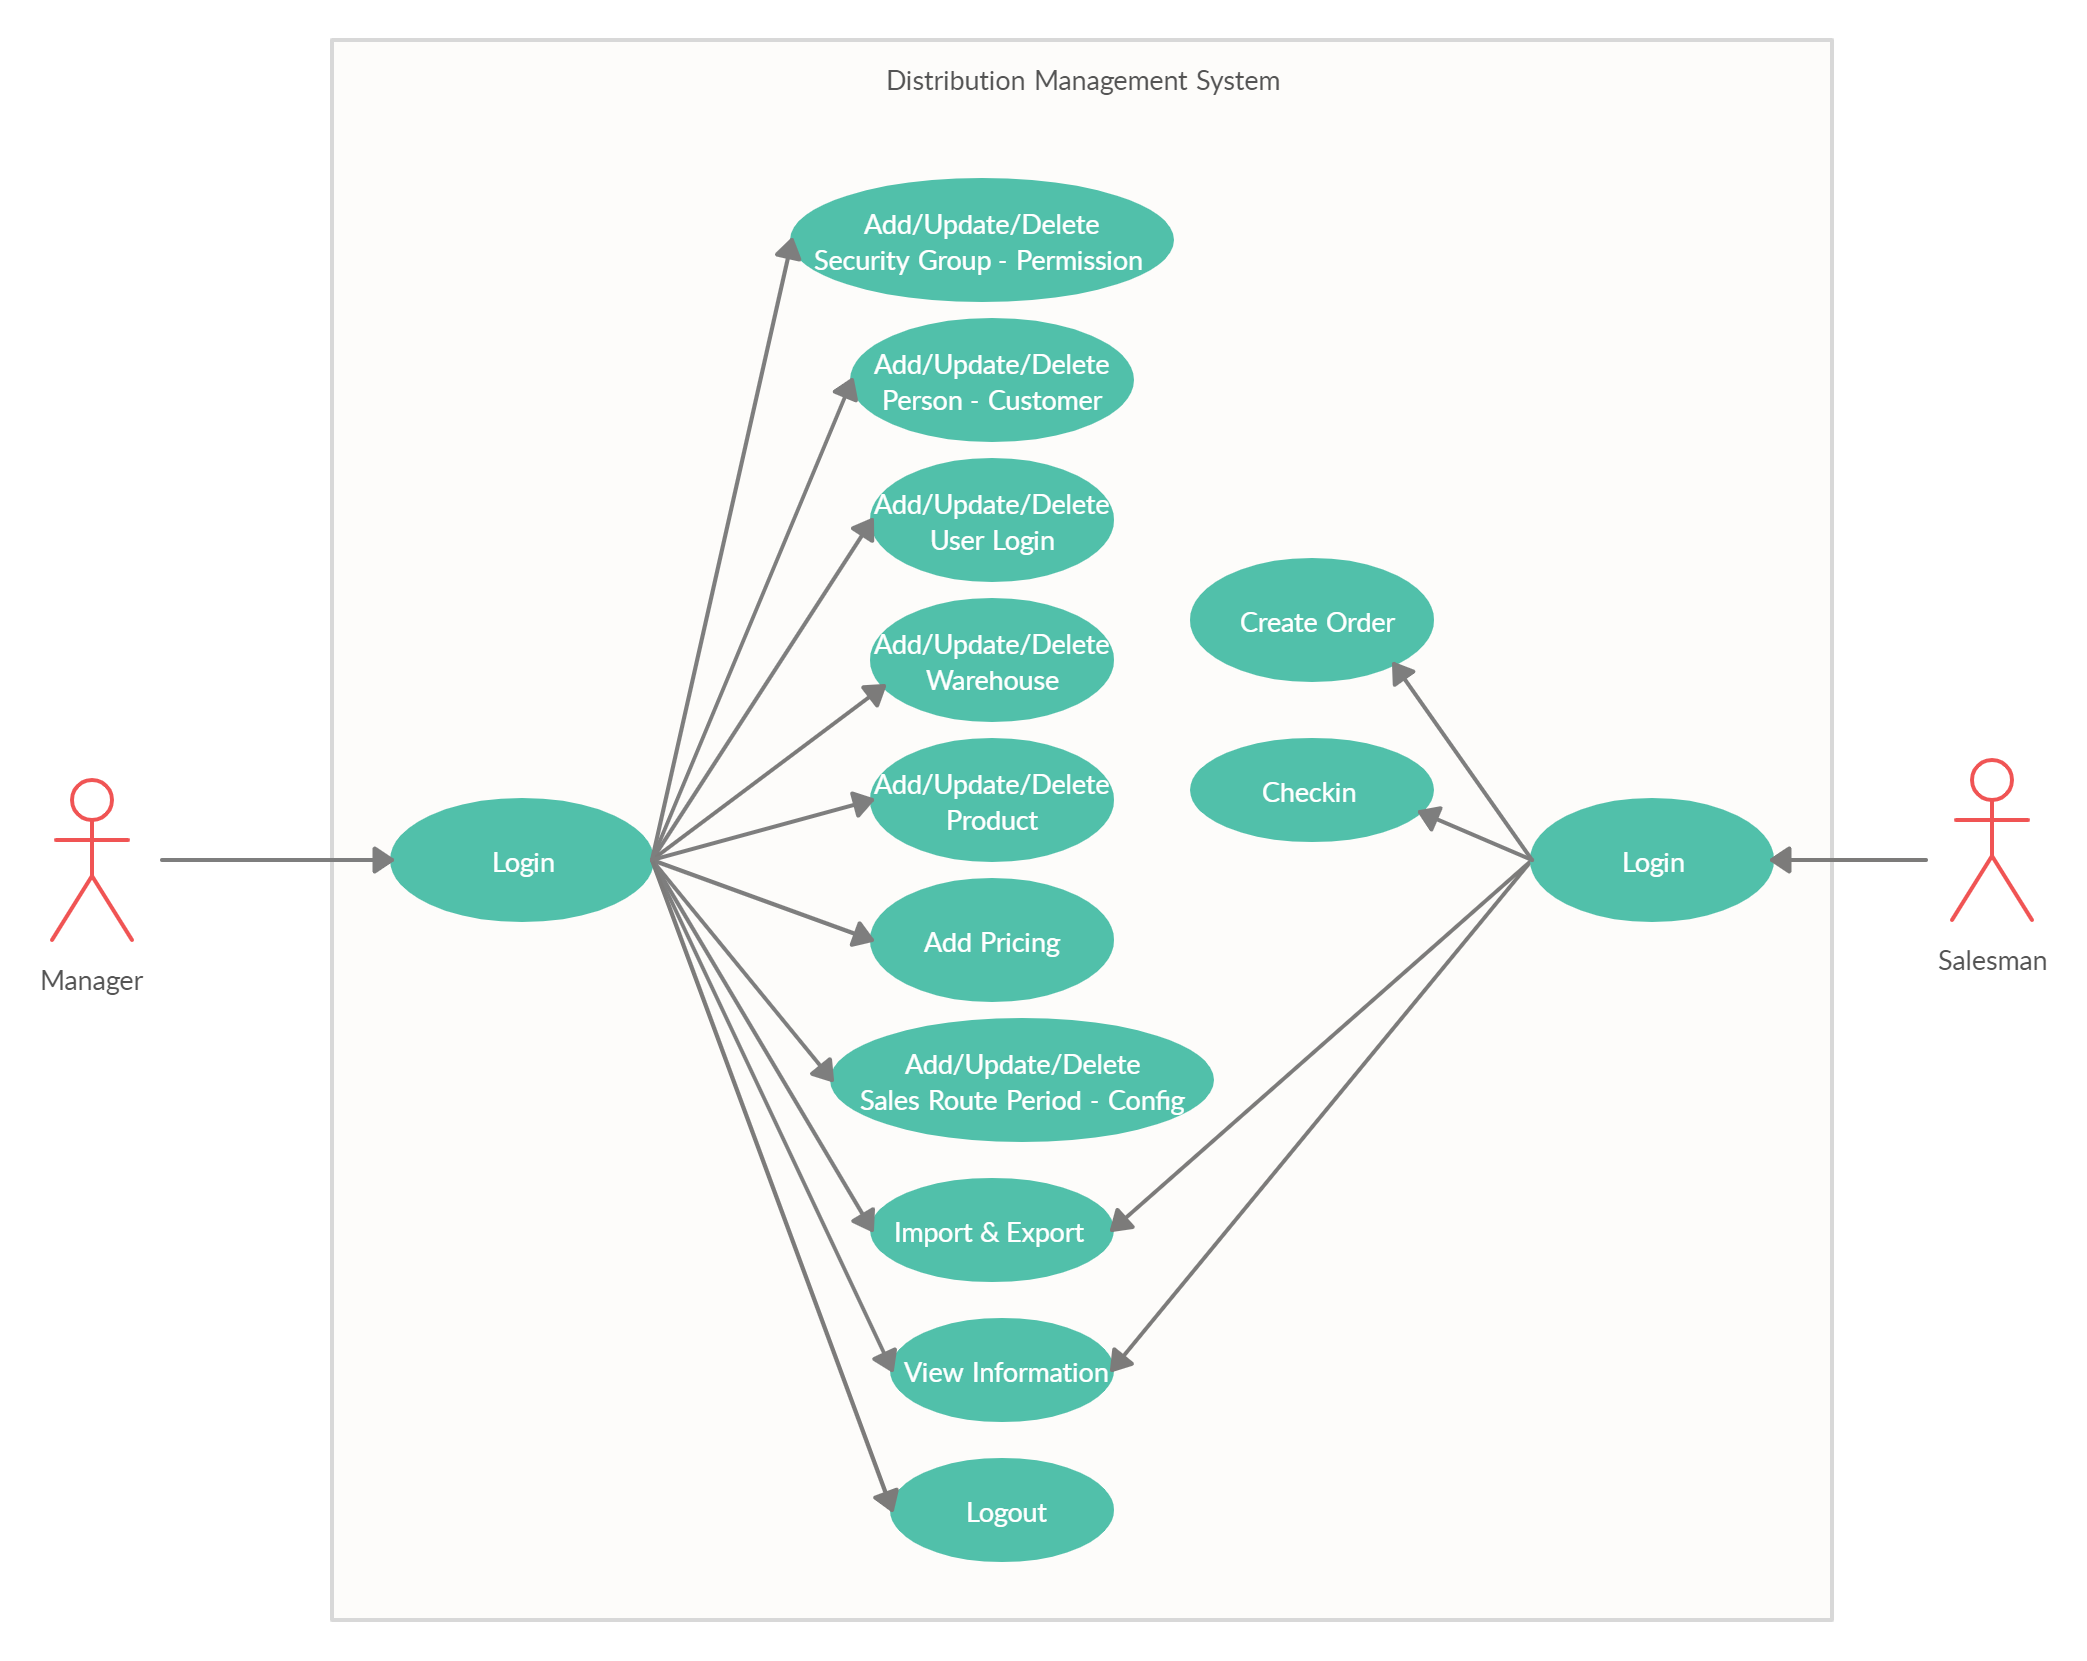
\includegraphics[width=12cm]{images/use-case/use-case-summary.jpg}
    \caption{Biểu đồ use case tổng quan}
\end{figure}

Hai tác nhân chính trong biểu đồ use case tổng quan
là người quản lý (manager) và nhân viên bán hàng (salesman).
Người quản lý ở đây là từ dùng chung, đại diện cho những người
quản lý nghiệp vụ riêng (quản lý sản phẩm, quản lý hàng tồn kho,
quản lý kho, quản lý giao dịch, quản lý tuyến bán hàng).
Người quản lý sau khi đăng nhập vào hệ thống có thể thực hiện
các nghiệp vụ quản lý như thêm / sửa / xóa sản phẩm, người dùng, …
Nhân viên bán hàng sau khi đăng nhập có thể xem được lịch
trình di chuyển của mình, lên hóa đơn mua hàng, check-in.

\subsection{Biểu đồ use case phân rã các chức năng của hệ thống}
Trong phần này, em sẽ trình bày các ca sử dụng chính trong hệ
thống, đưa ra biểu đồ use case và biểu đồ hoạt động chỉ cách
thức tương tác của người dùng với giao diện hệ thống. Do nhiều thao
tác có tính chất tương đồng nên em sẽ đưa ra các biểu
đồ hoạt động điển hình, các thao tác khác được thực hiện tương tự.

\subsubsection{Quản lý người dùng và phân quyền}
Biểu đồ use case cho ca sử dụng quản lý người dùng

\begin{figure}[H]
\centering
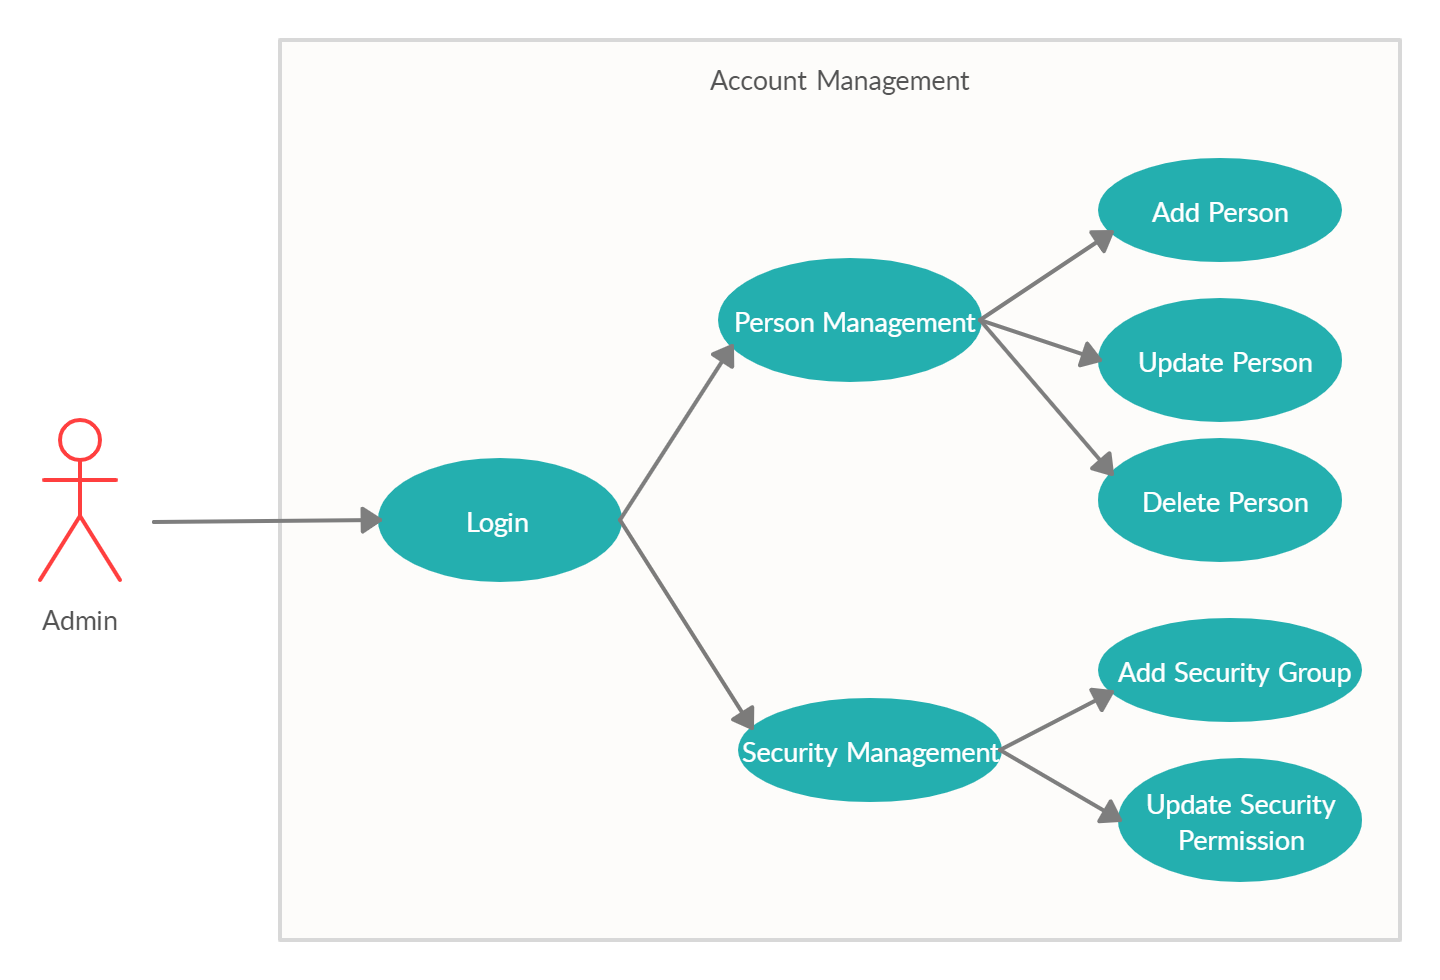
\includegraphics[width=12cm]{images/use-case/account-management.jpg}
\caption{Use-case quản lý người dùng}
\end{figure}

Người quản trị (admin) có thể quản lý các người dùng trong
hệ thống, quản lý quyền hạn của người dùng. Có thể thêm / sửa /
xóa người dùng, khách hàng, thêm / sửa quyền cho các người
quản lý cấp dưới.


Biểu đồ hoạt động cho các thao tác trong quản lý người dùng:
\begin{figure}[H]
\centering
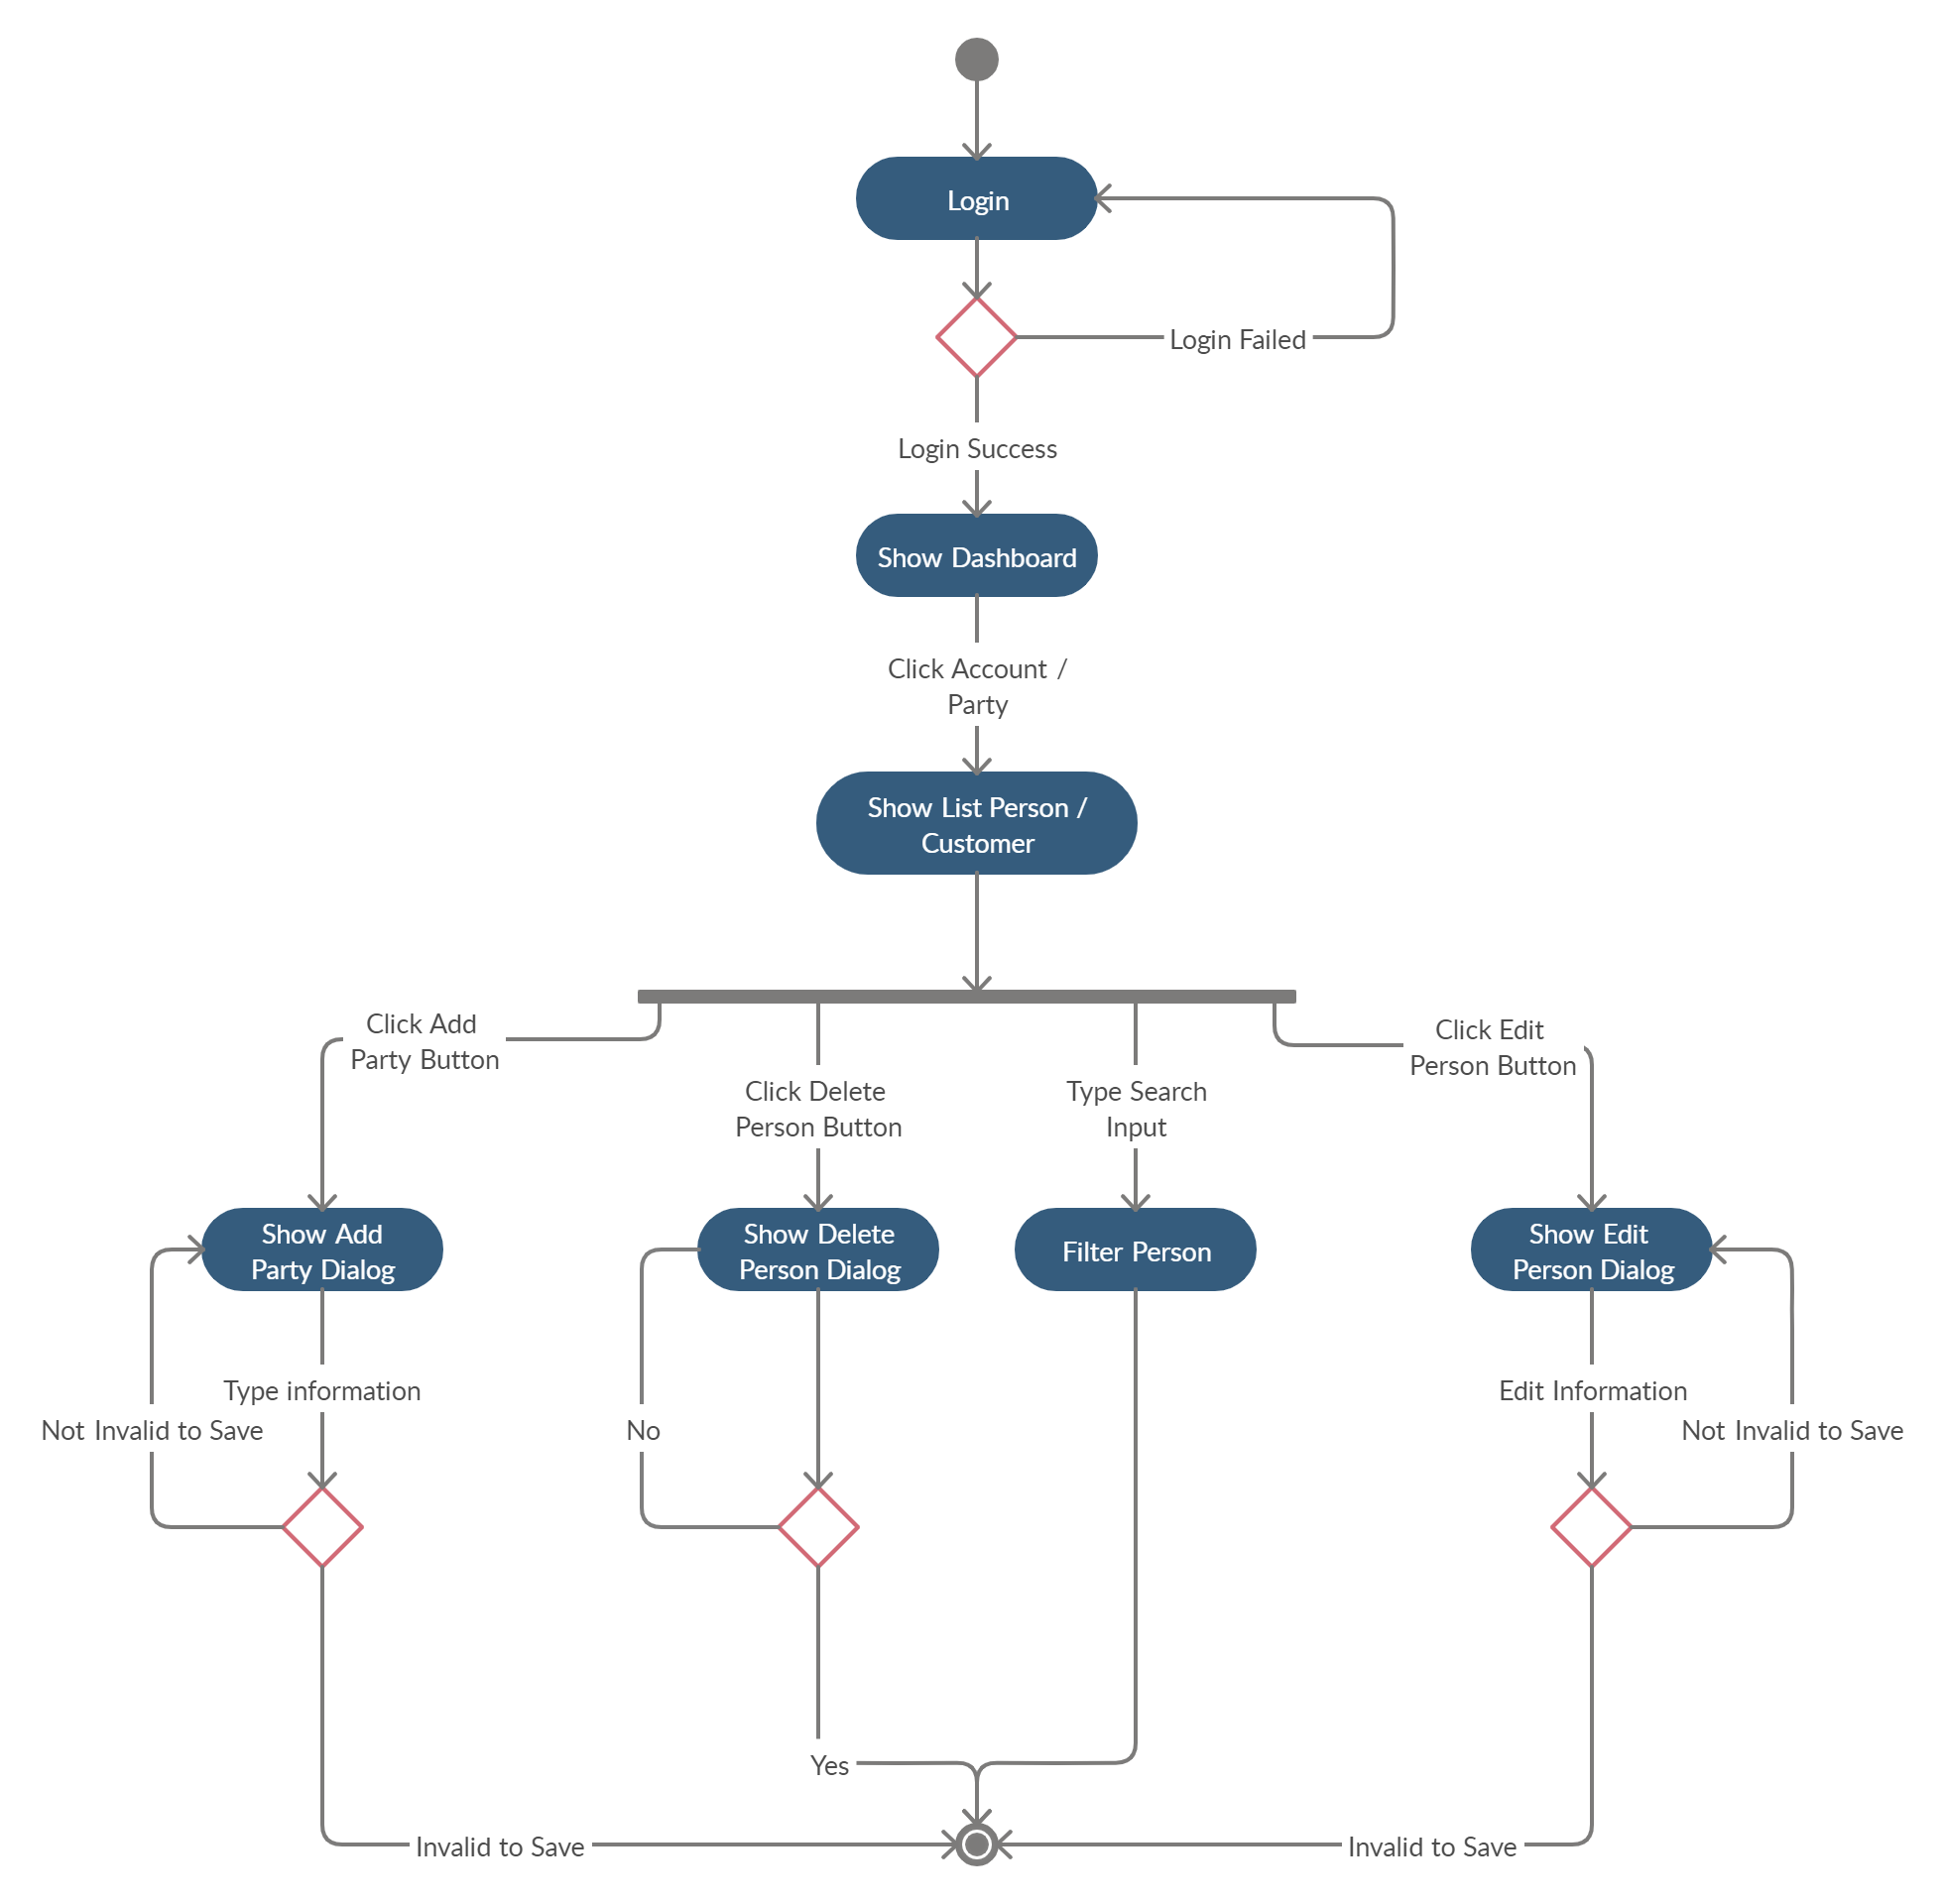
\includegraphics[width=15cm]
{images/activity-diagram/account-management.png}
\caption{Biểu đồ hoạt động ca sử dụng quản lý người dùng}
\end{figure}

Biểu đồ hoạt động cho thao tác phân quyền:
\begin{figure}[H]
\centering
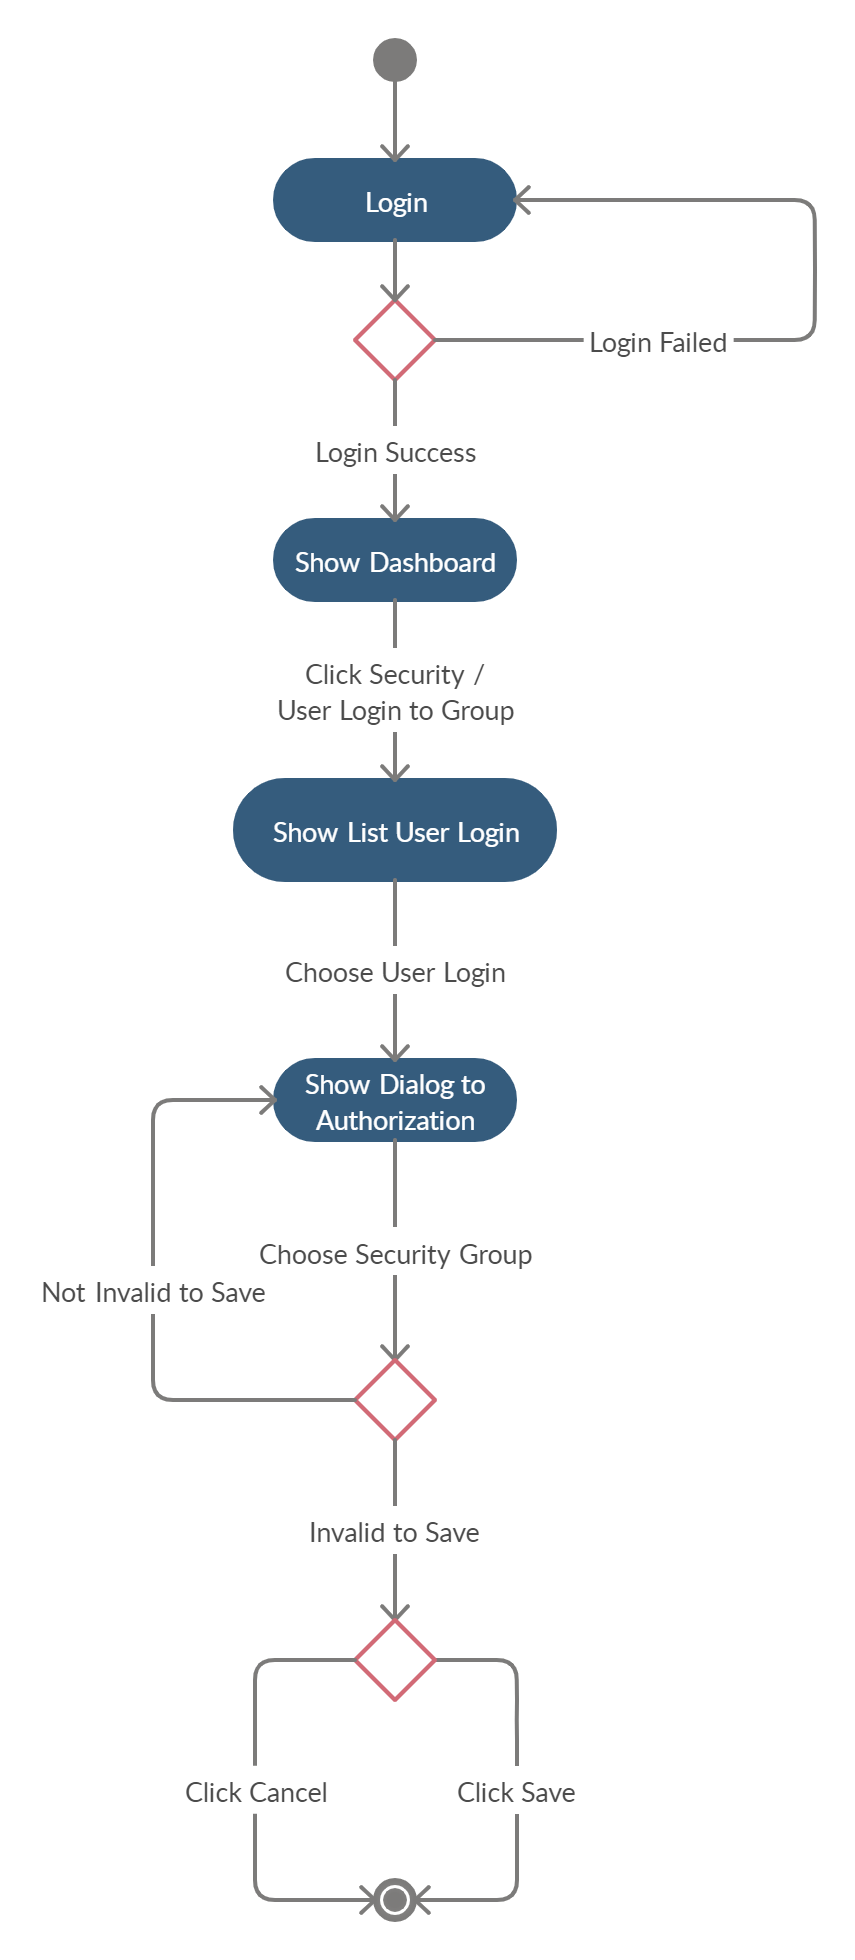
\includegraphics[width=7cm]
{images/activity-diagram/assign-permissions.png}
\caption{Biểu đồ hoạt động cho thao tác phân quyền}
\end{figure}

\subsubsection{Quản lý kho}
Biểu đồ use case cho ca sử dụng quản lý kho:
\begin{figure}[H]
\centering
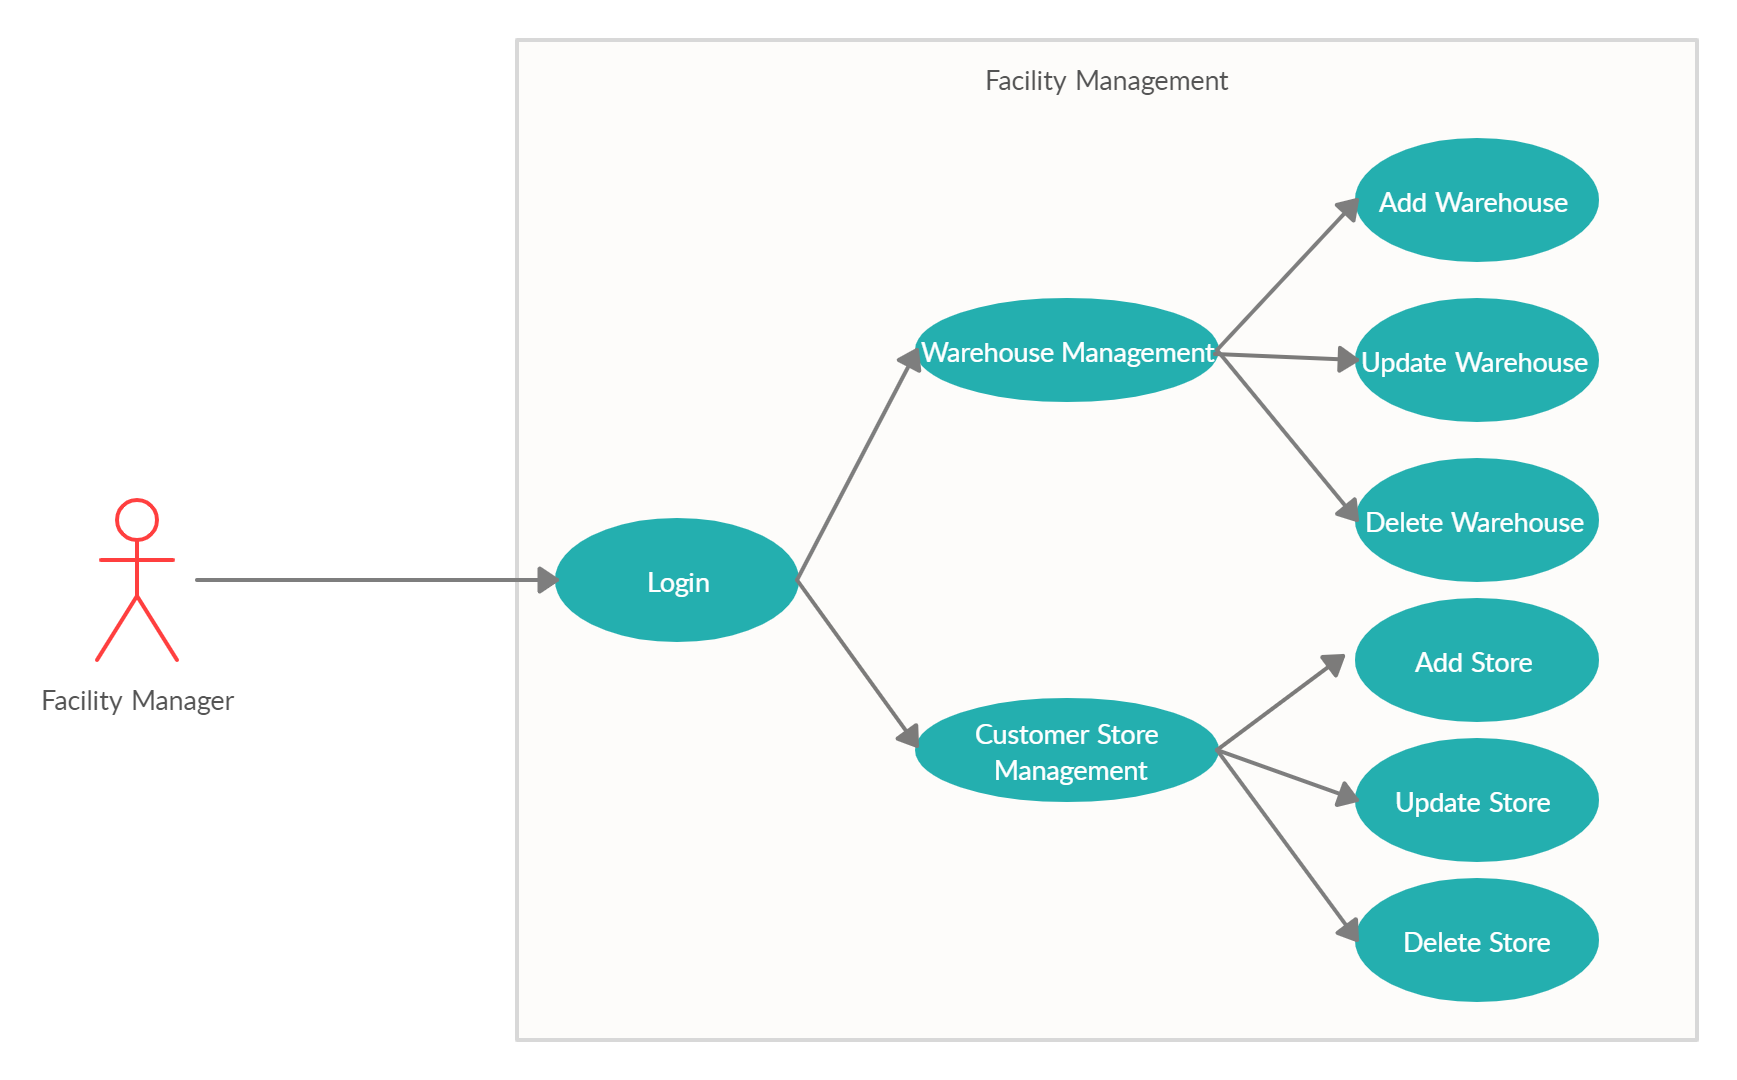
\includegraphics[width=14cm]{images/use-case/facility-management.jpg}
\caption{Use case quản lý kho}
\end{figure}

Người quản lý kho (Facility Manager) nắm được các thông tin
về kho của doanh nghiệp, tập đoàn và kho của cửa hàng bán lẻ,
có thể thêm / sửa / xóa các kho này. 

Biểu đồ hoạt động cho thao tác thêm cửa hàng bán lẻ:

\chapter{Các giải pháp, đóng góp nổi bật và minh họa các
chức năng của hệ thống}
\section{Vấn đề lựa chọn công nghệ}
\subsection{Công nghệ front-end}
Công nghệ front-end hiện nay phát triển rất nhanh và rộng.
Có rất nhiều các phương pháp tiếp cận lập trình front-end, đi kèm
là rất nhiều các thư viện, ngôn ngữ, framework,
công cụ hỗ trợ. Mỗi một công nghệ mới ra đời đều đáp ứng
tốt nhu cầu thị trường tại thời điểm đó và
khắc phục được những nhược điểm của các công nghệ cũ.
Ví dụ trước đây một lập trình viên front-end chỉ cần
biết về HTML, CSS mà JavaScript để xây dựng một trang web
thỏa mãn nhu cầu người dùng. Tuy nhiên theo thời gian, nhu cầu
người dùng về tính tương tác của trang web ngày càng cao dẫn
tới sự phát triển mạnh mẽ của ngôn ngữ JavaScript và các thư viện,
framework xây dựng từ đó như thư viện JQuery, EmberJS hay các
thư viện / framework nổi tiếng được dùng phổ biến hiện nay là
ReactJS, Angular, VueJS.

Dựa theo xu thế công nghệ hiện nay, chúng tôi chọn ReactJS – Redux để
xây dựng phần giao diện khi mà thư viện này có một cộng đồng lớn
và được Facebook phát triển. React-Router để định tuyến, xây dựng
Single Page Application, i18next để triển khai đa ngôn ngữ,
Redux-Saga để xử lý middleware,
gửi request và nhận api từ back-end server. 

\subsection{Công nghệ back-end}
Về phần back-end, ban đầu chúng tôi chọn Java Spring để xây dựng.
Java Spring cũng là một framework mạnh mẽ để xây dựng webserver.
Tuy nhiên, Java Spring phù hợp với xây dựng các ứng dụng web
monolithic (đơn khối) hơn là xây dựng theo mô hình microservices
đang trở thành xu hướng trong thời gian hiện nay. Một
hệ thống kiến trúc theo microservices thông thường sẽ
bao gồm nhiều các service nhỏ nhưng số lượng nhiều thì Java
Spring không phù hợp với những service đó do yêu cầu về tài
nguyên của ứng dụng Java là khá lớn. Vì vậy chúng tôi chọn
Go để xây dựng lại back-end server. Về cơ bản thì Go rất
phù hợp cho việc xây dựng các service trong microservices
do yêu cầu về tài nguyên nhỏ, ngoài ra Go còn hỗ trợ tốt xử
lý đa luồng với Goroutine và Chanel đã trình bày ở phần
công nghệ back-end nên
sẽ có thể tăng số request phục vụ tại cùng một thời điểm của hệ thống.

\subsection{Công nghệ Full Text Search}
Như đã đề cập ở phần công nghệ, trong đồ án này chúng tôi sử
dụng tính năng Full Text Search đã có trên PostgreSQL kết hợp
với sử dụng Index cho các câu truy vấn tìm kiếm người dùng,
khách hàng, tài khoản, tên sản phẩm, \ldots Ban đầu chúng tôi
chọn ElasticSearch cho tính năng này, tuy nhiên để sử dụng
ElasticSearch thì dữ liệu trong PostgreSQL phải được sao lưu
sang ElasticSearch. Để thực hiện việc sao lưu này có thể thực
hiện trên code của web server hoặc sử dụng hệ thống
Change Data Capture như Debezium.

Nếu thực hiện trên code thì không đảm bảo được dữ liệu
ở PostgreSQL và trên ElasticSearch là giống nhau. Đồng thời
sẽ làm code của web server trở nên phực tạp hơn do vừa phải quan
tâm đến dữ liệu của PostgreSQL vừa cả dữ liệu trên ElasticSearch.

Nếu sử dụng hệ thống Change Data Capture như Debezium
thì sẽ giải quyết được hai vấn đề trên, tuy nhiên lại làm hệ thống
phức tạp lên rất nhiều vì phải triển khai cả Kafka làm
kênh trung gian truyền dữ liệu từ PostgreSQL sang ElasticSearch.
Việc sử dụng một công nghệ phức tạp như vậy vượt quá giới
hạn thời gian cho đồ án này. Vì vậy chúng tôi sử dụng cách đơn giản
hơn là tính năng Full Text Search tích hợp sẵn trong PostgreSQL,
khi đó sẽ không phải xét đến vấn đề sao
lưu và tính nhất quán của dữ liệu.

\section{Chức năng phân quyền động}
Phân quyền là tính năng không thể thiếu được trong các trang mang
tính chất quản trị, mỗi người cần phải được giới hạn trong truy cập.
Ví dụ không thể để một nhân viên bán hàng sử dụng được tính năng
quản lý sản phẩm hay giá sản phẩm. Do đó dựa trên các tính năng
đã phân tích như quản lý phân quyền, quản lý sản phẩm, quản lý tài khoản,
quản lý kho, quản lý tuyến bán hàng, … chúng tôi phân chia người dùng
hệ thống vào các security\_group, mỗi security\_group lại có một tập
quyền (permissions). Hệ thống sẽ dựa vào các permission mà người
dùng có để xác định xem họ có thể truy
cập được vào tính năng đó hay không.

\begin{table}[H]
\centering
\begin{tabular}{| m{5cm} | m{11cm} |}
\hline
\textbf{security\_group} & \textbf{security\_permission} \\
\hline
ADMIN &
VIEW\_EDIT\_PARTY, VIEW\_EDIT\_USER\_LOGIN,
VIEW\_EDIT\_SECURITY\_GROUP,
VIEW\_EDIT\_SECURITY\_PERMISSION \\
\hline
PRODUCT\_MANAGER &
VIEW\_EDIT\_PRODUCT \\
\hline
SALES\_MANAGER & 
VIEW\_EDIT\_ORDER \\
\hline
FACILITY\_MANAGER & 
VIEW\_EDIT\_FACILITY \\
\hline
INVENTORY\_MANAGER & 
IMPORT \\
\hline
EXPORT\_MANAGER &
EXPORT \\
\hline
SALESMAN\_MANAGER &
VIEW\_EDIT\_SALESMAN \\
\hline
SALESMAN &
SALESMAN\_CHECKIN \\
\hline
\end{tabular}
\caption{Security\_group và permission tương ứng}
\end{table}

Khi một người dùng được thêm vào hệ thống, họ sẽ được cấp một
user\_login (hiểu như là username), giả sử người này là quản lý
sản phẩm thì sẽ được cấp một quyền VIEW\_EDIT\_PRODUCT, nếu người này
có khả năng quản lý rộng hơn làm được cả nhập kho thì sẽ cấp thêm
quyền IMPORT, … Đường dẫn (url) sẽ được gán theo permission để
kiểm soát truy nhập. Ví dụ PRODUCT\_MANAGER muốn xem danh sách các
sản phẩm thì phải truy cập url có dạng …/view-product,
url này chỉ được truy cập khi có quyền VIEW\_EDIT\_PRODUCT.

% \section{Chức năng phân cụm cửa hàng}
% Đây là một tính năng hoàn toàn mới, theo
% tìm hiểu và khảo sát của chúng tôi
% thì chưa có trên các phần mềm quản lý phân phối hiện nay. Xuất phát
% từ ý tưởng các nhân viên bán hàng hằng ngày phải thăm các cửa hàng bán
% lẻ. Vậy làm thế nào có thể tối ưu được quãng đường di chuyển của nhân
% viên, để họ có thể di chuyển một cách dễ dàng nhất. Và chúng tôi đã đưa
% ra tính năng này, với mục đích là đưa ra gợi ý về các cụm
% cửa hàng gần nhau, giúp người quản lý tuyến bán hàng chọn ra các
% tuyến bán hàng phù hợp.

% Sử dụng thuật toán phân cụm K-Means với đầu vào là N cửa
% hàng bán lẻ trong hệ thống, và K cụm (do người quản lý tuyến
% chỉ định). Đầu ra của thuật toán là K cụm, trong đó là vị trí
% các cửa hàng gần nhau. Tuy nhiên khoảng cách sử dụng không phải là
% khoảng cách Euclidean, mà là khoảng cách Haversine – công thức
% tính khoảng cách giữa hai điểm trên tọa độ thực tế
% (dựa trên kinh độ và vĩ độ).

% Công thức Haversine tính khoảng cách giữa 2 
% điểm $(x_1, y_1)$, $(x_2, y_2)$ trong không gian sử
% dụng kinh độ và vĩ độ:
% \begin{align*}
% &\Delta x = x_1 - x_2 \\
% &\Delta y = y_1 - y_2 \\
% &a = \sin^2 \left( \frac{\Delta x}{2} \right)
%     + \cos \left( x_1 \right) \times \cos \left( x_2 \right) 
%     \times \sin^2 \left( \frac{\Delta y}{2} \right)
%     \\
% &c = 2 \times \arcsin \left( \sqrt{a} \right ) \\
% &d = R \times c
% \end{align*}
% Trong đó: $x_1$, $x_2$ là kinh độ, $y_1$ $y_2$ là vĩ độ, tính bằng radian.
% R là bán kính trái đất (xấp xỉ $6,371$ km). $d$ là khoảng cách cần tìm.

\section{Minh họa các chức năng của hệ thống}
\begin{figure}[H]
\centering
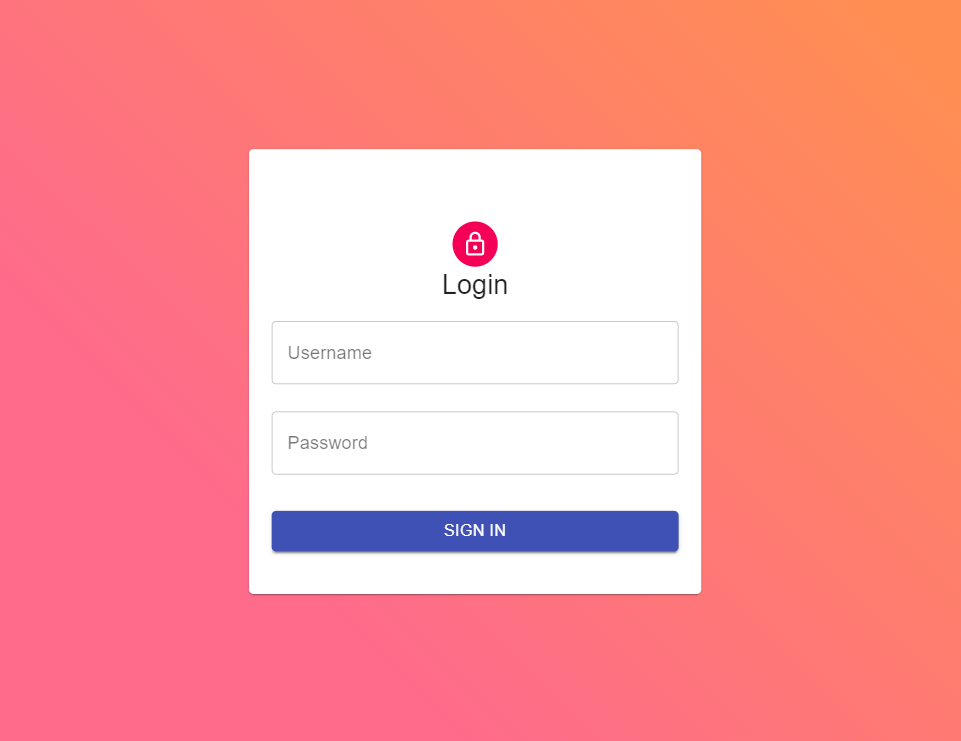
\includegraphics[width=12cm]{images/demo/login.png}
\caption{Chức năng đăng nhập}
\end{figure}

\begin{figure}[H]
\centering
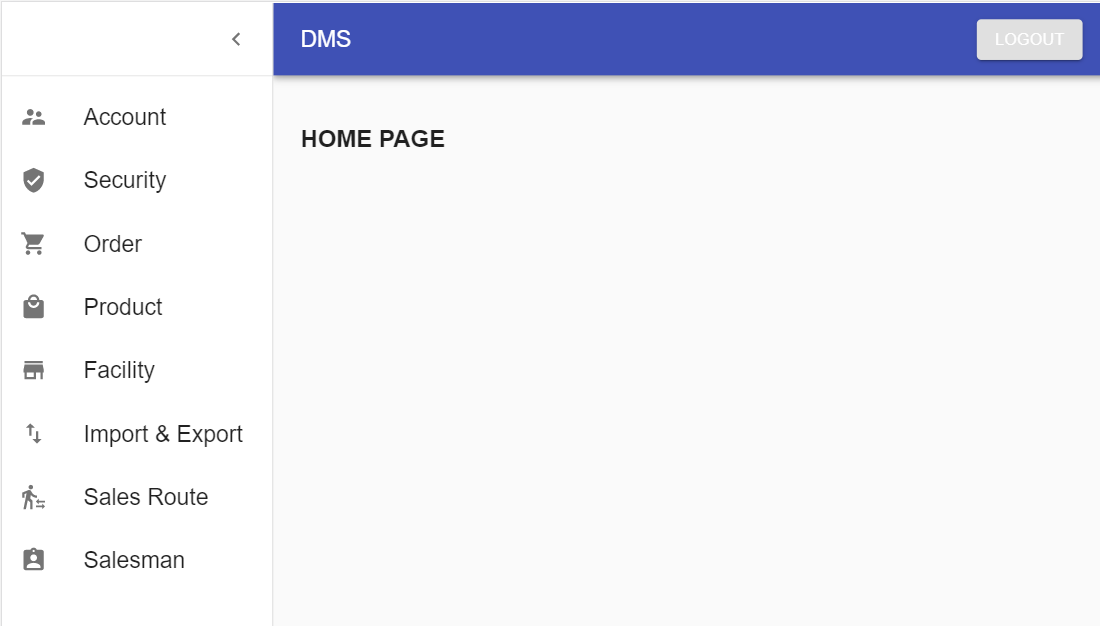
\includegraphics[width=15cm]{images/demo/home-page.png}
\caption{Giao diện trang chủ hệ thống}
\end{figure}

\begin{figure}[H]
\centering
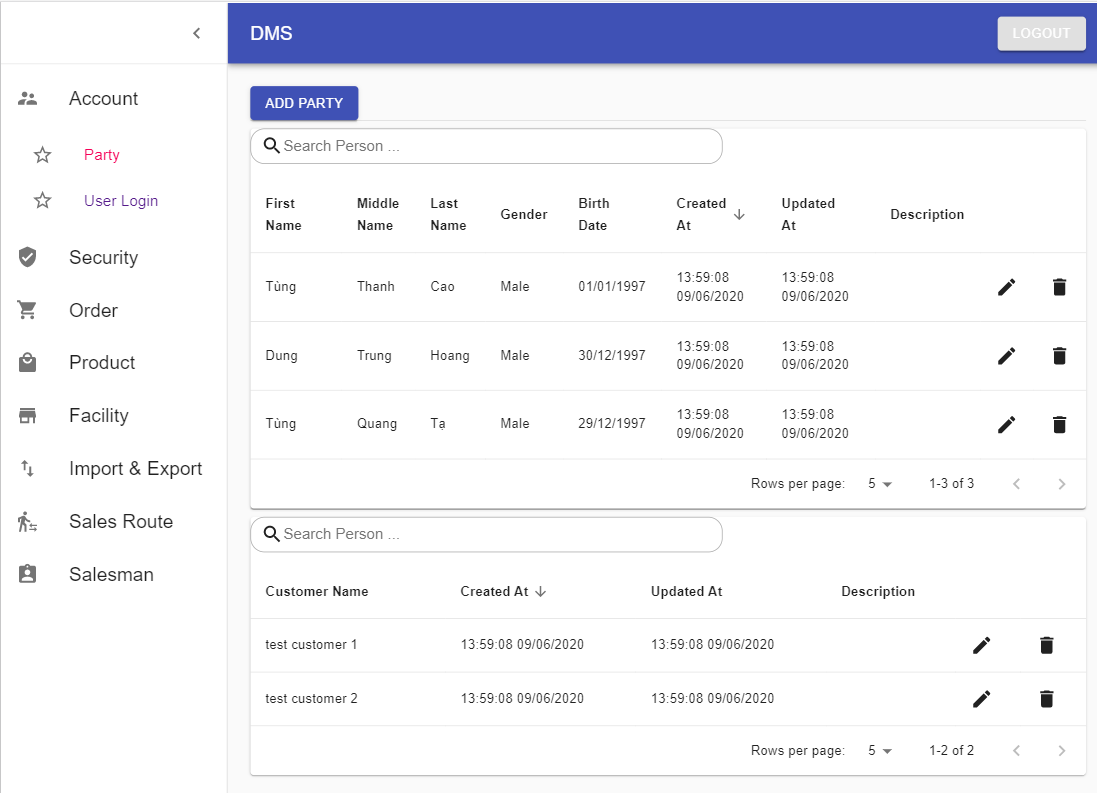
\includegraphics[width=15cm]{images/demo/party-manage.png}
\caption{Quản lý người dùng}
\end{figure}

\begin{figure}[H]
\centering
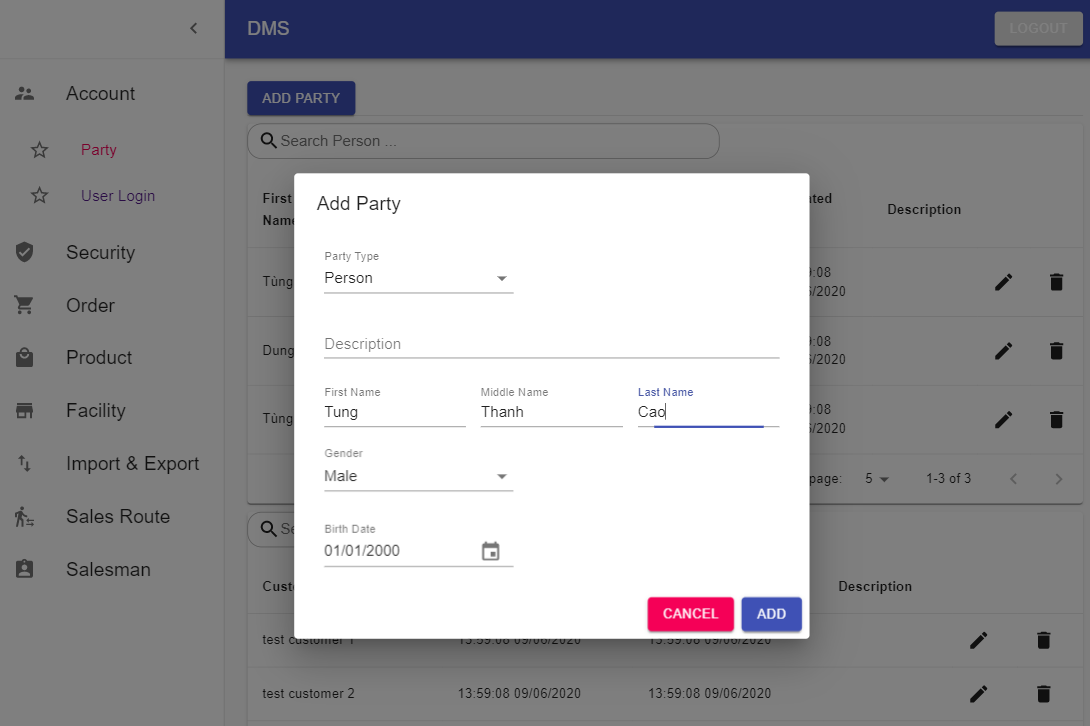
\includegraphics[width=15cm]{images/demo/add-party.png}
\caption{Thêm người dùng / khách hàng}
\end{figure}

\begin{figure}[H]
\centering
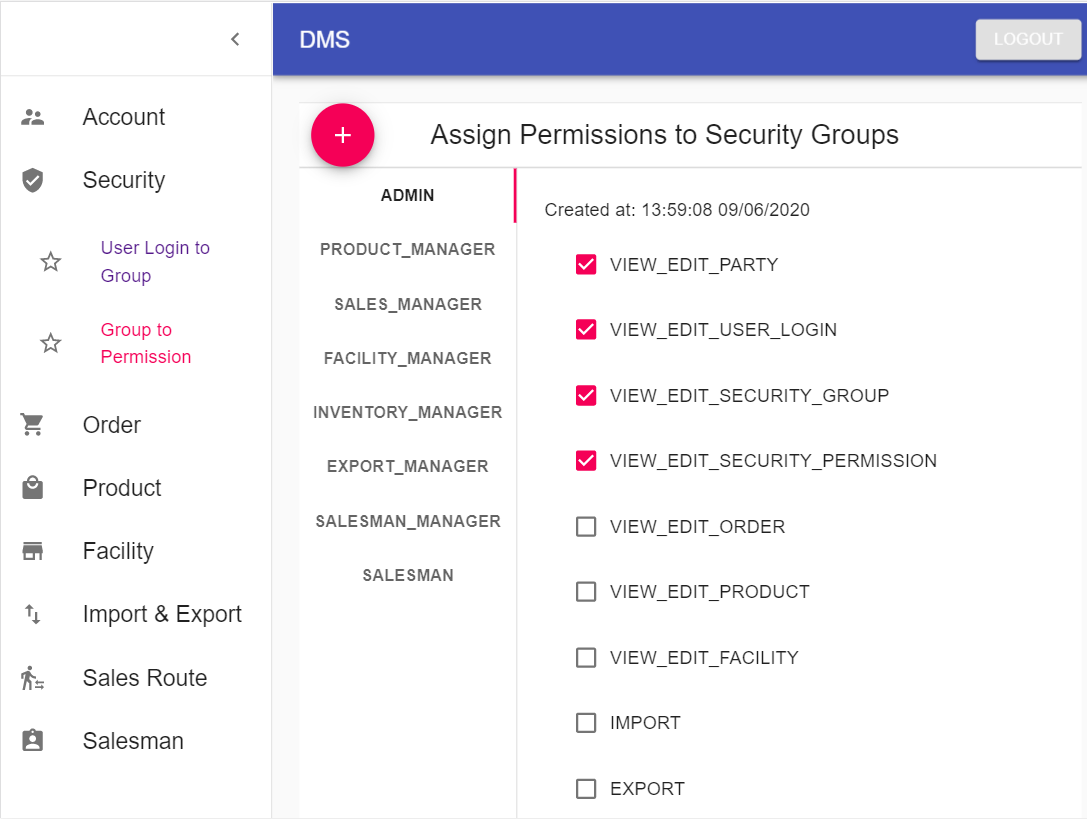
\includegraphics[width=15cm]{images/demo/group-to-permission.png}
\caption{Quản lý các nhóm quyền}
\end{figure}

\begin{figure}[H]
\centering
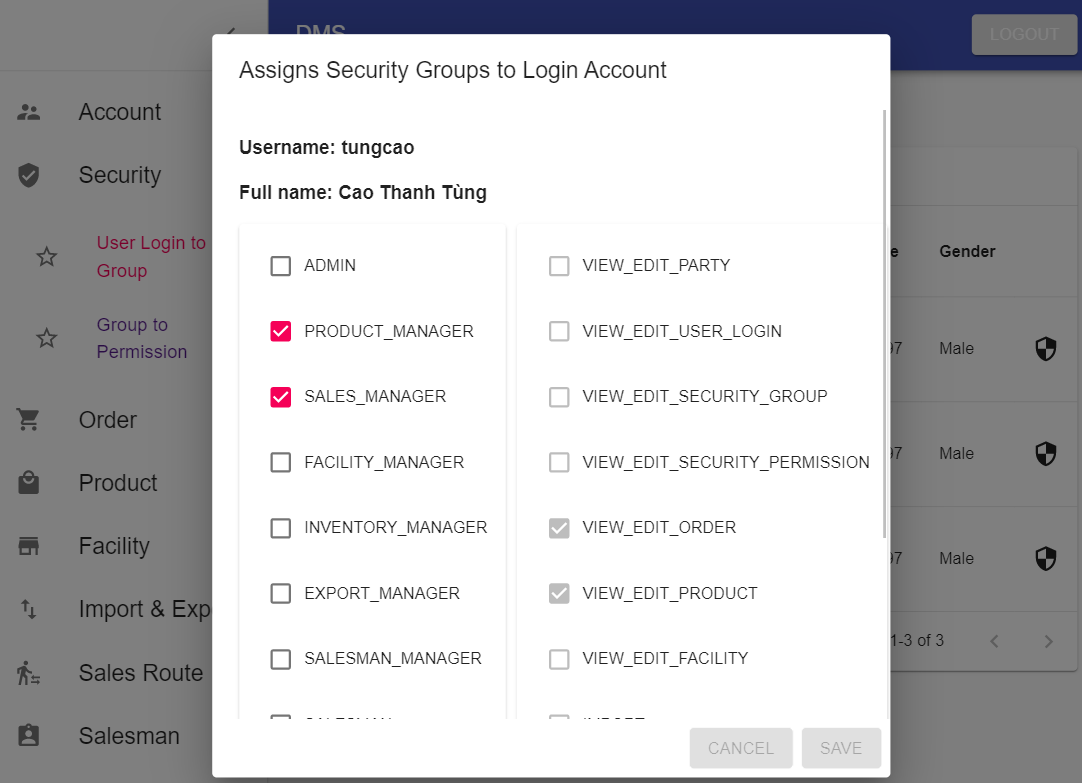
\includegraphics[width=15cm]{images/demo/user-login-to-group.png}
\caption{Gán quyền cho tài khoản người dùng}
\end{figure}

\begin{figure}[H]
\centering
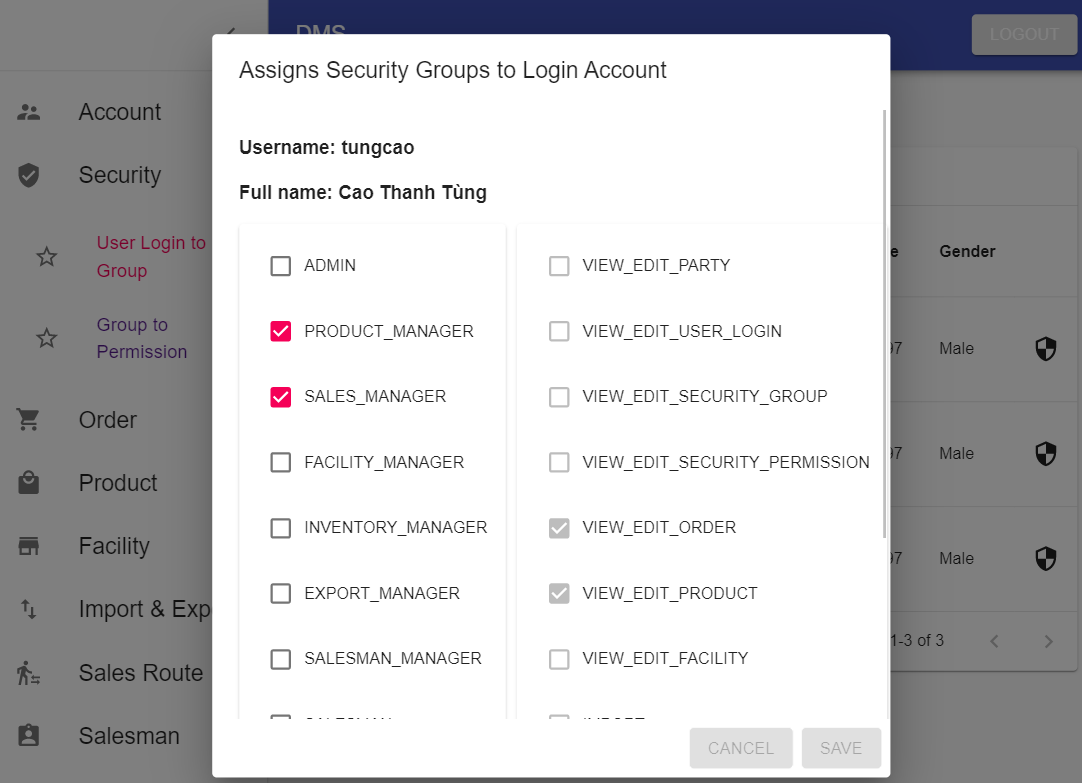
\includegraphics[width=15cm]{images/demo/user-login-to-group.png}
\caption{Gán quyền cho tài khoản người dùng}
\end{figure}

\begin{figure}[H]
\centering
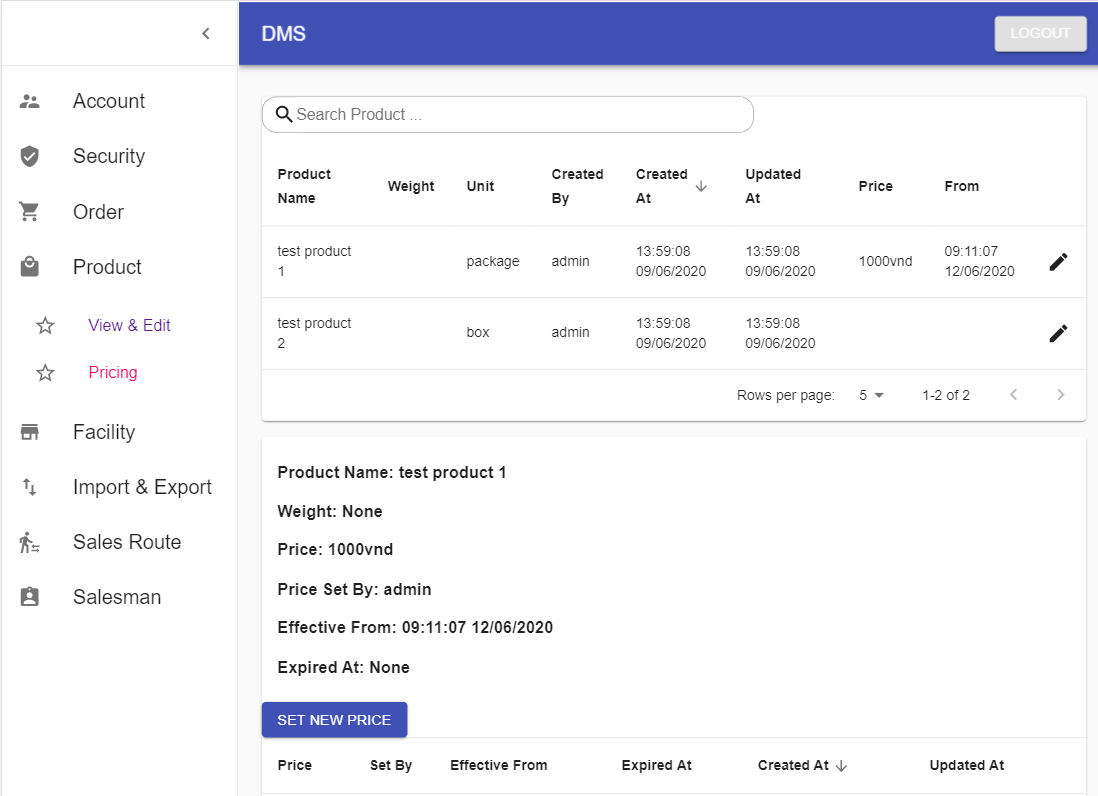
\includegraphics[width=15cm]{images/demo/product-price.png}
\caption{Quản lý giá của các sản phẩm}
\end{figure}

Tạo đơn hàng mới phải qua các bước như chọn khách hàng
(để giao hàng đến), chọn kho chứa hàng hóa, chọn hàng
hóa, nhập địa chỉ (nếu có hoặc chọn kho của cửa hàng).
\begin{figure}[H]
\centering
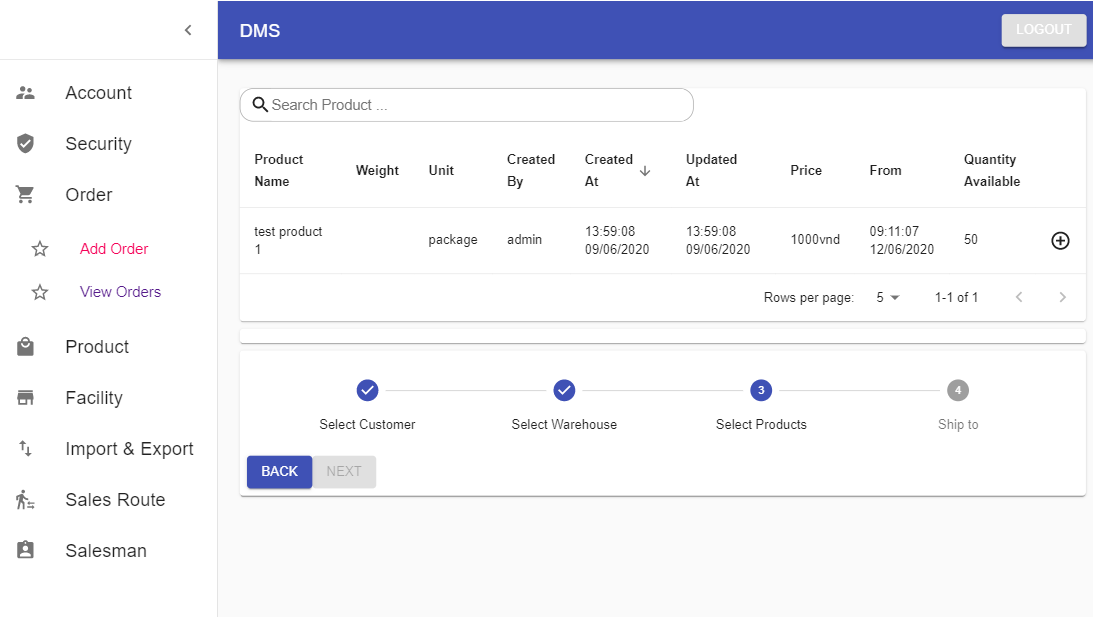
\includegraphics[width=15cm]{images/demo/add-order.png}
\caption{Tạo đơn hàng}
\end{figure}

\begin{figure}[H]
\centering
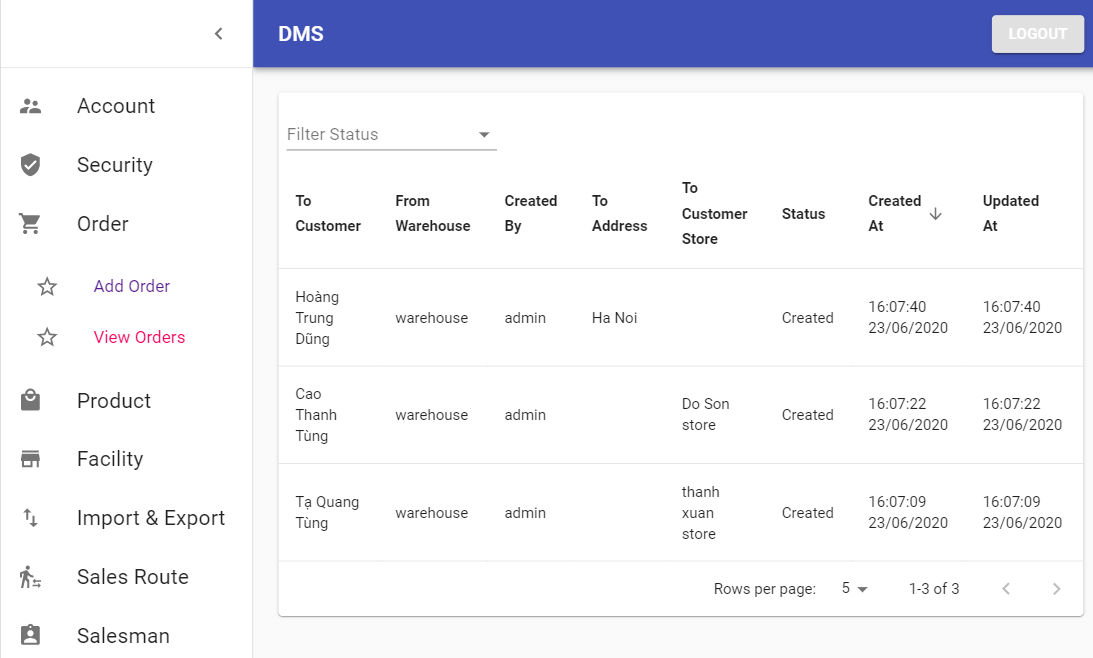
\includegraphics[width=15cm]{images/demo/view-orders.png}
\caption{Hiển thị đơn hàng}
\end{figure}

\begin{figure}[H]
\centering
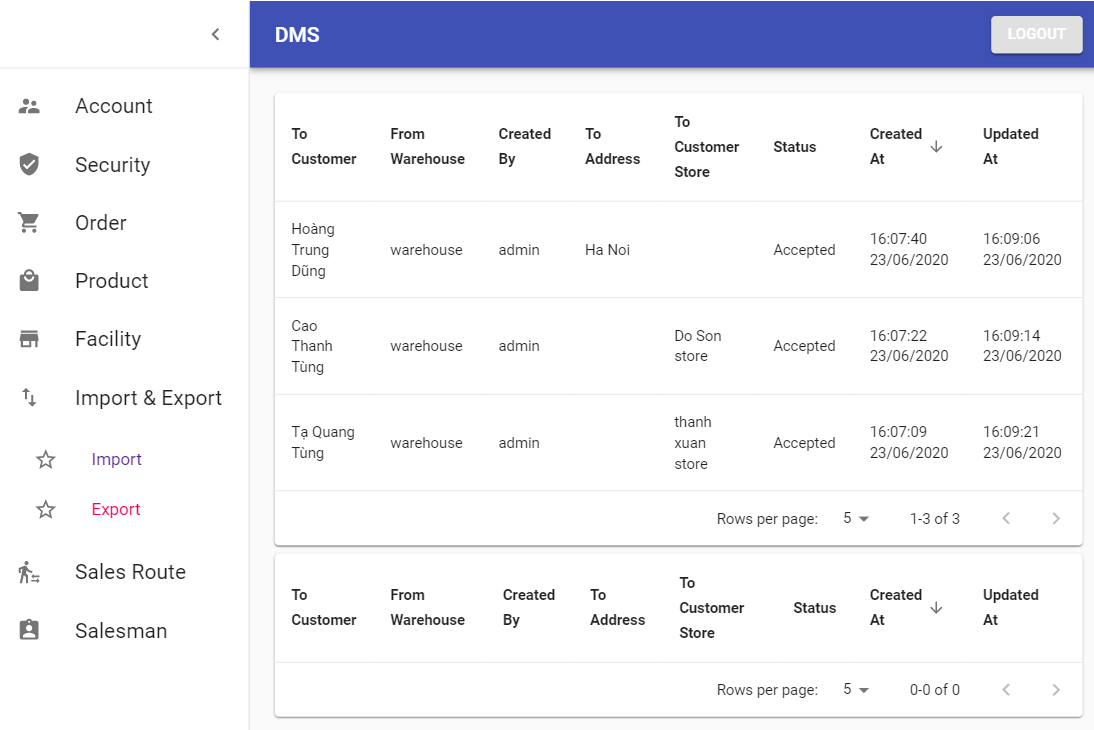
\includegraphics[width=15cm]{images/demo/view-export.png}
\caption{Quản lý xuất kho}
\end{figure}

% Chức năng thêm mới cửa hàng bán lẻ, hỗ trợ bản đồ
% Google Map để xác định vị trí.
% \begin{figure}[H]
% \centering
% 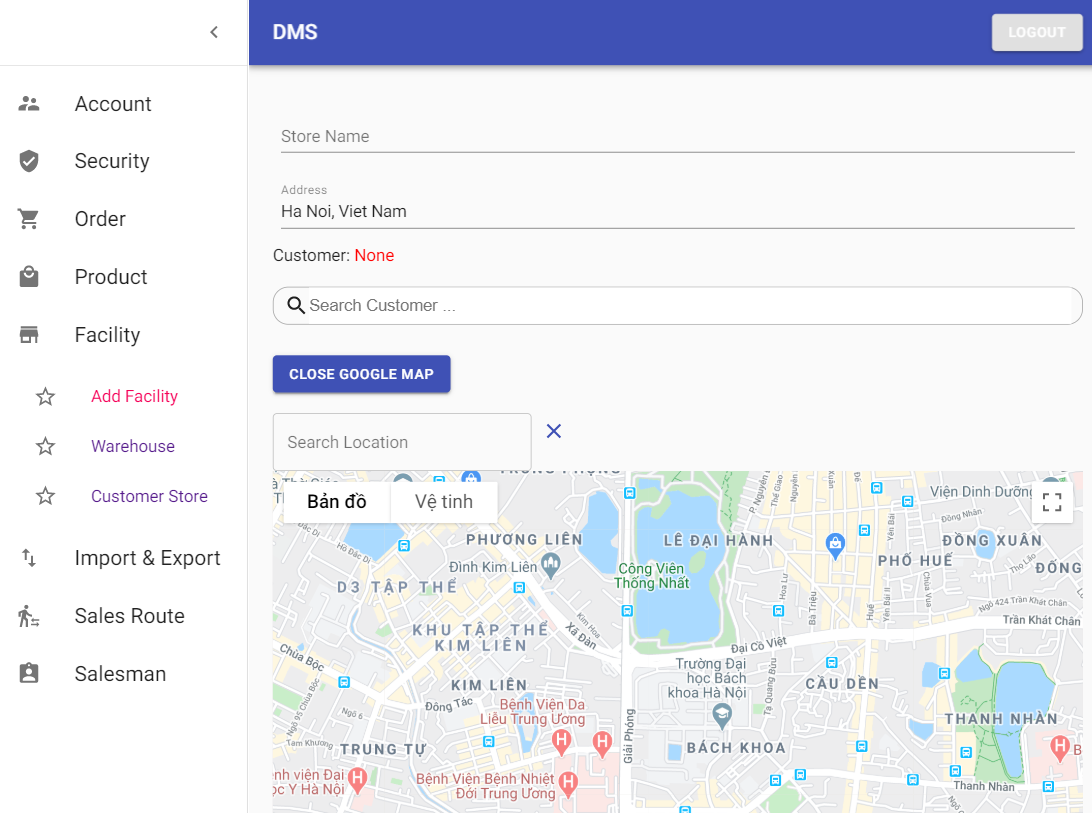
\includegraphics[width=15cm]{images/demo/add-customer-store.png}
% \caption{Thêm mới một cửa hàng bán lẻ}
% \end{figure}

% Chức năng tạo lịch trình tuyến bán hàng, sử dụng thuật toán
% K-Means phân cụm các cửa hàng bán lẻ, từ đó người quản lý
% chọn ra tuyến bán hàng phù hợp nhất cho nhân viên bán hàng.
% \begin{figure}[H]
% \centering
% 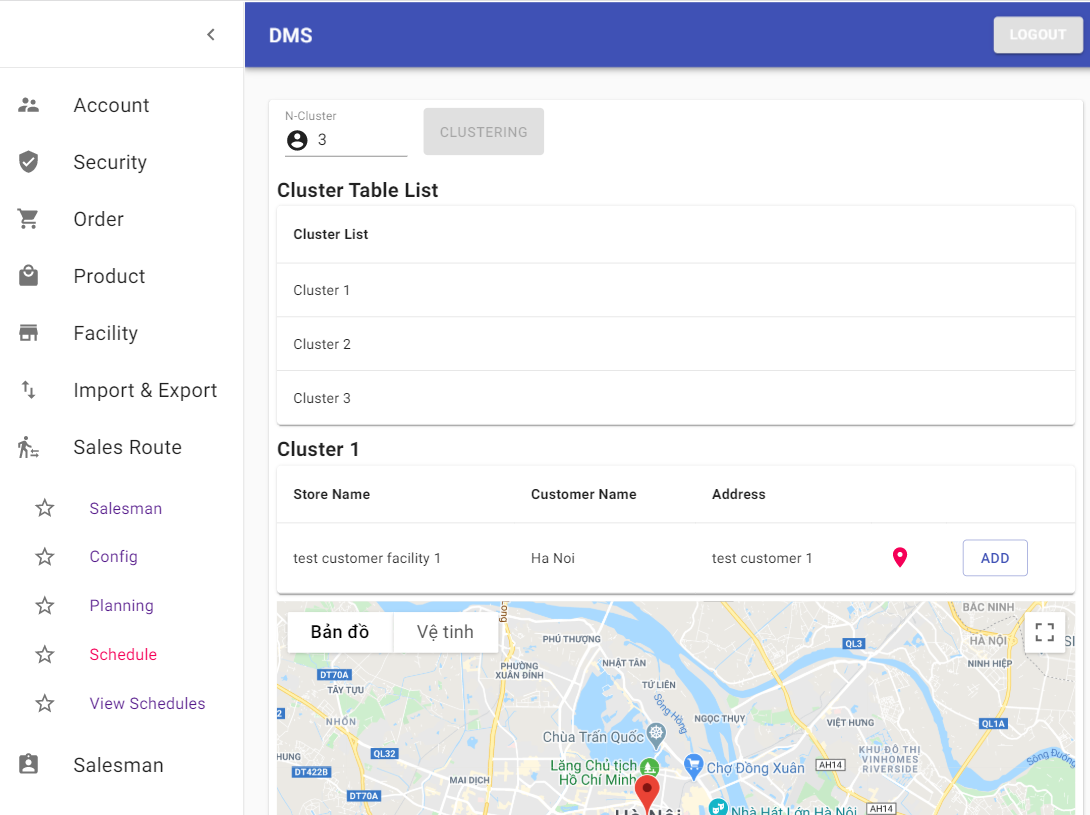
\includegraphics[width=15cm]{images/demo/add-schedule.png}
% \caption{Tạo lịch trình tuyến bán hàng}
% \end{figure}

% \begin{figure}[H]
% \centering
% 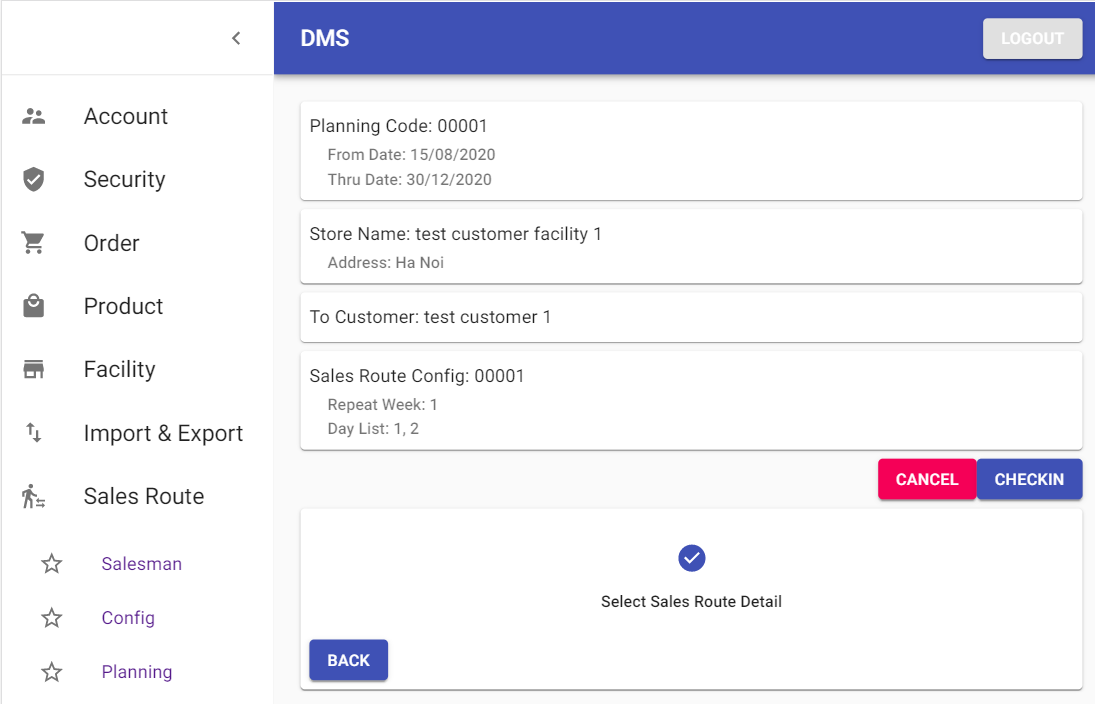
\includegraphics[width=15cm]{images/demo/salesman-checkin.png}
% \caption{Salesman check-in}
% \end{figure}

\chapter{KẾT LUẬN VÀ HƯỚNG PHÁT TRIỂN}
\section{Kết luận}
Đồ án được thực hiện trong khuôn khổ của nhóm với hai sinh viên
nhắm tới mục tiêu thiết kế và xây dựng hệ thống với các tính năng
cơ bản nhất của một hệ thống quản lý phân phối bao gồm quản lý
khách hàng, quản lý nhân viên bán hàng, quản lý tuyến bán hàng,
xây dựng kế hoạch tuyến bán hàng, lên đơn hàng, quản lý xuất kho,
tồn kho.

Trong đồ án này, chúng tôi đặt mục tiêu xây dựng phân hệ
quản lý sản phẩm, quản lý đơn hàng, quản lý xuất nhập kho
của các sản phẩm. Kết quả đạt được của đồ án là phân hệ
quản lý đơn hàng và xuất nhập kho với
khoảng 40 use-case, được phát triển
dựa trên công nghệ Go phía server và ReactJS/Redux phía giao
diện. Phân hệ đã sử dụng công nghệ container Docker,
nền tảng Container orchestration engine là Kubernetes và
sử dụng dịch vụ cloud Microsoft Azure để triển khai
và thử nghiệm ứng dụng. Quá trình triển khai ứng dụng đã
được hoàn thiện.

Qua quá trình tìm hiểu và thực hiện hệ thống quản lý phân phối,
nghiên cứu quy trình và các chức năng nghiệp vụ, thiết kế giao
diện, cơ sở dữ liệu thì phần mềm nhóm chúng tôi tạo ra đã cơ bản hoàn
thiện, đáp ứng đủ những ca sử dụng như thiết kế. Phần giao diện
viết bằng ReactJS theo chuẩn Single Page Application, thiết kế theo
phong cách Material Design. 

Để trở thành một dự án khả thi trong thực tế thì ứng dụng cần phải
khắc phục nhiều hạn chế. Phần giao diện còn tương đối sơ
sài vì chưa có nhiều thời gian chỉnh sửa,
việc này đòi hỏi nhiều thứ như nên thiết kế trang chủ thế nào,
thiết kế logo, vị trí đầu trang và chân trang cần những thông tin
như thế nào, hiệu ứng trượt dọc, dropdown, … Ở các công ty thì họ có
kỹ sư thiết kế UX/UI, một đội photoshop, một đội dựng giao diện
và hiệu ứng, do đó đây là hạn chế thứ hai của nhóm chúng tôi. Hạn chế
tiếp theo là, dù đã sử dụng webpack để nén mã nguồn, Single Page
để tối ưu tốc độ tải của trang web nhưng do dùng nhiều thư viện
vẫn chưa thực sự kiểm soát được hiệu năng của front-end, Lý do là
sử dụng thư viện Material-UI chiếm phần lớn kích thước của file
JavaScript được biên dịch ra.

% Sau khi thực hiện đồ án tốt nghiệp, chúng tôi nhận thấy đã có
% nhiều tiến bộ về cả kiến thức và kỹ năng.
% Chúng tôi đã được thực hành nhiều
% công nghệ mới về web front-end, web back-end, cơ sở dữ liệu;
% biết được những công nghệ này là lợi thế lớn khi đi làm sau này.
% Học được cách xử lý tình huống khi gặp lỗi (lỗi cú pháp lập trình,
% lỗi logic, …), tỉ mỉ hơn khi thiết kế giao diện, học được cách tối ưu
% hiệu năng front-end, thuật toán phân cụm dữ liệu. Về kỹ năng thì
% chúng tôi đã học được về kỹ năng làm việc nhóm khi mà mỗi người làm một
% nhiệm vụ khác nhau, quản lý code qua các branch trên GitHub;
% kỹ năng tìm kiếm tài liệu trên Google, tìm đúng từ khóa,
% đúng nội dung cần tìm; … Và hơn nữa sau khi làm đồ án, chúng tôi đã có
% một sản phẩm thật, chạy được đáp ứng đủ yêu cầu về nghiệp vụ
% cho hệ thống quản lý phân phối trong chuỗi cung ứng.

\section{Hướng phát triển của đồ án trong tương lai}
Là một phần mềm mang tính thương mại nên chúng tôi rất muốn có thể
triển khai ứng dụng trong thực tế. Để làm được việc này thì trước tiên
chúng tôi cần hoàn thiện phần giao diện của mình, sau đó là chỉnh sửa lại
các tính năng đã có cho dễ sử dụng hơn, đẹp hơn; khắc phục
các hạn chế đã nêu ở trên; thiết kế thêm các tính năng mới.

Chúng tôi cũng mong muốn được thử nghiệm hiệu năng với nhiều tình
huống thực tế khác và đánh giá tác động của Full Text Search
trong việc tìm kiếm và chèn, sửa, xóa các bản ghi. Đồng thời,
chúng tôi rất có thể triển khai trên các dịch vụ cloud khác như
Google Cloud hay Amazon Web Service hay triển khai nó trên
một cluster tự quản lý.


\appendix
% appendices come here

\label{sect:bib}
\bibliographystyle{plain}
\bibliography{thesis}
%\addcontentsline{toc}{chapter}{Bibliography}
%\bibliographystyle{alpha}
%\bibliography{bibliography/bibliography}

\end{document}
